\documentclass[a4paper,11pt]{article}


\pdfoutput=1

\usepackage[a4paper,left=2.73cm,right=2.7cm,top=3cm,bottom=3.5cm]{geometry}

%\usepackage[T1]{fontenc} 
\usepackage[latin2]{inputenc}
\usepackage{graphicx}
\usepackage{epsfig}
%\usepackage{rotating}
\usepackage{amssymb}
\usepackage{amsfonts}
%\usepackage{dsfont}
%\usepackage{psfrag}
\usepackage{amsmath,euscript,array,mathrsfs}
%\usepackage{bbold} %HB: this made \mathbb{R} look strange
\usepackage{epsf}
\usepackage{slashed}
\usepackage{comment}
\usepackage{colortbl}
\usepackage{cite}
\usepackage{parskip}
\usepackage{mathtools}
\usepackage{upgreek}

\usepackage{caption,subcaption,wrapfig}
\usepackage[colorlinks=true,linktocpage=true,linkcolor=blue,citecolor=blue]{hyperref}

\usepackage{tikz}
\usetikzlibrary{decorations.markings,decorations.pathmorphing}

\newcommand{\be}{\begin{equation}}
\newcommand{\ee}{\end{equation}}
\newcommand{\beqs}{\begin{eqnarray}}
\newcommand{\eeqs}{\end{eqnarray}}
\newcommand{\parent}[1]{\left(#1\right)}
\newcommand{\tb}{t_\textrm{bounce}}




\newcommand{\lsim}{\mathrel{\raisebox{-
.6ex}{$\stackrel{\textstyle<}{\sim}$}}}
\newcommand{\gsim}{\mathrel{\raisebox{-
.6ex}{$\stackrel{\textstyle>}{\sim}$}}}

\newcommand{\Tr}{{\rm Tr}}

\newcommand{\arcsinh}{\rm arcsinh}
\newcommand{\arctanh}{\rm arctanh}
\newcommand{\dd}{\mathrm{d}}
\newcommand{\sac}{\, , \qquad}

\newcommand{\AAA}{\mathcal{A}}
\newcommand{\FF}{\mathcal{F}}
\newcommand{\OO}{\mathcal{O}}
\newcommand{\GG}{\mathcal{G}}
\newcommand{\MM}{\mathcal{M}}
\newcommand{\LL}{\mathcal{L}}
\newcommand{\BB}{\mathcal{B}}
\newcommand{\B}{\mathbb{B}}
\newcommand{\C}{\mathbb{C}}
\newcommand{\CP}{\mathbb{C}\mathbb{P}}

\newcommand{\Bconf}{\mathbb{B}_8^{\rm{conf}}}
\newcommand{\BOP}{\mathbb{B}_8^{\rm{OP}}}

\def\di{\mbox{d}}
\def\r{\rho}
\def\cO{{\cal O}}

\setlength{\parindent}{2em}
\numberwithin{equation}{section}
\allowdisplaybreaks

\begin{document}



 \begin{titlepage}

\thispagestyle{empty}

$\,$

%\begin{flushright}
%\hfill{ICCUB-19-015}
%\end{flushright}

\vspace{40pt}  
	 
\begin{center}

{\huge \textbf{Cauchy Evolution of Asymptotically Global AdS Spacetimes with No Symmetries}}

\vspace{30pt}
		
{\large \bf Hans Bantilan, Pau Figueras,  Lorenzo Rossi}
		

\vspace{25pt}


{\normalsize  
School of Mathematical Sciences, Queen Mary University of London, Mile End Road, London E1 4NS, United Kingdom}

\vspace{10pt}
\texttt{h.bantilan@qmul.ac.uk}, \texttt{p.figueras@qmul.ac.uk}, \texttt{l.rossi@qmul.ac.uk}


\vspace{40pt}
				
\abstract{
%We present the first proof-of-principle Cauchy evolutions of asymptotically AdS spacetimes with no symmetries, employing a numerical scheme based on the generalized harmonic form of the Einstein equations.
%The main difficulty in removing all symmetry assumptions is in finding a gauge choice of generalized harmonic source functions that is consistent with the AdS reflective boundary conditions.
%We detail a prescription to obtain an explicit gauge choice that achieves this in four dimensions.
%We suggest that our prescription would lead to stable evolution also in settings with $d\geq 4$ spacetime dimensions, various couplings with matter fields, and many (if not all) types of global or non-global Poincar\'{e} coordinates.
%We apply the prescription to perform the first long-time 3+1 simulations of four dimensional spacetimes with a negative cosmological constant in global (asymptotically) Cartesian coordinates, using initial data sourced by a massless scalar field.
%We present preliminary results of Cauchy evolution of horizonless data, as well as data that undergoes gravitational collapse.
%These results are a direct precursor to important specialized studies of AdS dynamics with no symmetry assumptions.
We present the first proof-of-principle Cauchy evolutions of asymptotically AdS spacetimes with no imposed symmetries, employing a numerical scheme based on the generalized harmonic form of the Einstein equations.
In this scheme, the main difficulty in removing all symmetry assumptions can be phrased in terms of finding a set of generalized harmonic source functions that are consistent with AdS boundary conditions.
We detail an explicit set of source functions that achieves fully general evolution in four dimensions.
A similar prescription should also lead to stable evolution in higher spacetime dimensions, various couplings with matter fields, and on the Poincar\'{e} patch.
We apply this scheme to obtain the first long-time stable 3+1 simulations of four dimensional spacetimes with a negative cosmological constant, using initial data sourced by a massless scalar field.
We present preliminary results of gravitational collapse and the subsequent quasi-normal ringdown to a static black hole in the bulk, mirrored by evolution towards a homogeneous state on the boundary.
These results are a direct precursor to important specialized studies of AdS dynamics with no symmetry assumptions.}

%\vspace{30pt}

%\noindent{Keywords}: AdS, generalized harmonic, 3+1, superradiance, gravitational collapse

%\noindent\textcolor{red}{This colour is for something we should discuss whether to add or not.}

\end{center}
%\vspace{40pt}

\end{titlepage}


\tableofcontents

% Uncomment for Submitted to journal title message
%\submitto{\JPA}
%
% Uncomment if a separate title page is required
%\maketitle
% 
% For two-column output uncomment the next line and choose [10pt] rather than [12pt] in the \documentclass declaration
%\ioptwocol

\hrulefill
\vspace{10pt}
%\noindent

%%%%%%%%%%%%%%%%%%%%%%%%%%%%%%%%%%%%%%%%%%%%%%%%
\section{Introduction}
%%%%%%%%%%%%%%%%%%%%%%%%%%%%%%%%%%%%%%%%%%%%%%%%

Anti-de Sitter (AdS) space has in recent years proven to be a particularly exciting theoretical laboratory for studying the strong-field regime of General Relativity (GR).
AdS with reflective boundary conditions plays the role of a box that naturally keeps propagating waves confined to its interior, where they are perpetually interacting.
Thus, even the smallest perturbations in AdS can enter the strong-field regime, where qualitatively new gravitational phenomena emerge.
One of the most important of these is gravitational collapse -- the growth of curvatures that eventually leads to the formation of a singularity in spacetime potentially associated with a black hole.
Obtaining the details of this fundamental process in full generality in AdS is an open problem. 
%\textcolor{blue}{{\bf PF:} I think that the previous paragraph is not correct given that the endpoint of superradiance isn't known. My alternative in red}
%Although it has not yet been proven mathematically, this process of black hole formation is expected to generically result in a rotating black hole that is characterized by two conserved numbers: total mass and total angular momentum. Small, rapidly rotating black holes in AdS are unstable due to a process known as superradiance -- the amplification of waves that scatter off a rotating object. Along with the box-like nature of AdS, this amplification leads to a runaway process whose endpoint is unknown. Finding this endpoint and the pathway by which it is reached is, again, an open problem.
Although it has not yet been proven rigorously, this process of black hole formation in asymptotically flat spaces is expected to generically result in a rotating black hole that is characterized by two conserved numbers: total mass and total angular momentum. In AdS, the endpoint is less clear since small, rapidly rotating black holes in AdS are unstable due to a process known as superradiance -- the amplification of waves that scatter off a rotating object. Along with the box-like nature of AdS, this amplification leads to a runaway process whose endpoint is unknown. 
%HB: last sentence breaks flow to next paragraph
%Hence, such small black holes are not expected to generically form as a result of gravitational collapse.  

In an unprecedented way, the simulation of asymptotically AdS spacetimes has also opened up the field of numerical relativity to the study of phenomena in areas beyond the traditional astrophysical setting. 
At the heart of this push to understand AdS is a deep connection between gravity in AdS to certain conformal field theories (CFT), now known as the AdS/CFT correspondence~\cite{Maldacena:1997re,Gubser:1998bc,Witten:1998qj}. 
Through this connection, the study of AdS spacetimes has become immediately relevant to fundamental questions in many areas in physics, such as fluid dynamics [cite], relativistic heavy ion collisions [cite], and superconductivity [cite] just to mention a few.
See, for example, [cite] for excellent reviews. 
The reason the study of AdS is crucial for our understanding of these phenomena is that AdS/CFT provides an important -- and in most cases the only -- window into the real-time dynamics of strongly interacting quantum field theories far from equilibrium. 
The dynamical far-from-equilibrium strongly interacting regime is precisely the one that is least explored and understood, and the one that has the best chance of making contact with certain experiments.
%Within GR, the dynamics of AdS provides a detailed look at how the Einstein equations behave in the fully non-linear regime and with non-trivial boundary conditions.
%This has led to important efforts to understand fundamental phenomena in gravity in this new setting.%, including gravitational collapse and superradiance. 

Our current understanding of gravity in AdS, however, remains limited for several reasons.
First, evolution in AdS is notoriously hard, in part because it is an initial-boundary value problem whose systematic study is still in its infancy. 
Cauchy evolution in AdS requires data to be prescribed not only at an initial space-like hypersurface, but also at spatial and null infinity which constitute the time-like boundary of an asymptotically AdS spacetime.
Second, the most interesting phenomena involve spacetimes that have very little or no symmetry, making these evolutions beyond the reach of most numerical codes. 
Third, for many of these phenomena, there is a variety of physical scales that must be adequately resolved to correctly capture the relevant physics.

%The main purpose of this article is to present the first proof-of-principle Cauchy evolution of asymptotically AdS spacetimes that has been achieved with no symmetry assumptions.
%The results presented here are based on a code that solves the Einstein equations coupled with matter fields for asymptotically AdS spacetimes with a generalized harmonic evolution scheme, with adaptive mesh refinement capabilities. 

The main purpose of this article is to present the first proof-of-principle Cauchy evolution of asymptotically AdS spacetimes that has been achieved with no symmetry assumptions, and describe the framework that makes Cauchy evolution in AdS possible in full generality.
The results presented here are based on a code with adaptive mesh refinement capabilities that solves the Einstein equations in generalized harmonic form for asymptotically AdS spacetimes, subject to reflective (i.e., Dirichlet) boundary conditions and with massless scalar field.
%\textcolor{red}{LR: I know that this is already mentioned in the last paragraph of the introduction but, since it is crucial for our scheme and that last paragraph is usually a place where authors just recap briefly what they said in the rest of the Introduction, I thought that we can consider saying that we use reflective BC here as well.} 
%with the generalized harmonic evolution scheme and adaptive mesh refinement capabilities.

%The main purpose of this article is to present the first proof-of-principle Cauchy evolution of asymptotically AdS spacetimes that has been achieved with no symmetry assumptions, by employing a code that solves the Einstein equations coupled with matter fields for asymptotically AdS spacetimes with a generalized harmonic evolution scheme, with adaptive mesh refinement capabilities.
%This code is the next step in an ongoing program initiated in \cite{Bantilan:2017kok} that uses (asymptotically) Cartesian coordinates in global AdS, now enabled with a breakthrough set of generalized harmonic source functions that is crucial in successfully stabilizing evolution in AdS with no symmetries.

\textcolor{blue}{{\bf PF:} we need a paragraph commenting on the ingoing scheme by Chesler and Yaffe. I'll give it a go later}

As [cite] demonstrate, a crucial requirement for obtaining stable evolution in AdS is a gauge choice that is consistent with the conditions imposed at the AdS boundary.
In most cases, a gauge choice leading to stable numerical evolution is typically found in spacetimes with a certain degree of symmetry.
%In this work, we detail a prescription that provides this gauge choice in a setting with no symmetry assumptions for $d=4$ spacetime dimensions.
In the present work, we detail a gauge choice in $d=4$ spacetime dimensions that leads to stable evolution in an asymptotically global AdS setting with no symmetry assumptions.
%various couplings with matter fields, and many (if not all) types of global or non-global Poincar\'{e} coordinates, as long as reflective Dirichlet boundary conditions are imposed at the AdS boundary (as explained in Section~\ref{subsec:cartevvarboucon}).
%If we wish to evolve points at the centre of the grid, which is the case when we want to analyze gravitational collapse and black hole formation, global (asymptotically) Cartesian coordinates (defined precisely in Section~\ref{subsec:asyAdS}) are of particular interest as the Courant-Friedrichs-Lewy (CFL) condition does not restrict the size of the time step too severely, \footnote{Unlike, for example, in spherical coordinates.} thus allowing reasonably affordable computing times for the simulations.
This work is a direct precursor to fully general studies of gravitational collapse and black hole formation in AdS.
Cartesian coordinates are suitable in this context, as they are regular everywhere, do not contain coordinate singularities, and do not have the well-known limitation suffered by spherical coordinates in the form of severely shorter time steps imposed by the Courant-Friedrichs-Lewy (CFL) condition. 
Similar coordinates were used in \cite{Bantilan:2017kok} to study the collapse of a massless scalar field in global $AdS_5$ with axisymmetry.
In anticipation of these fully general studies, we choose to write our prescription in terms of global Cartesian coordinates, and with second order finite difference derivative stencils to discretize the initial constraint equations and the evolution equations. Other choices of finite differencing discretization should also work. 

The rest of this article is organized as follows. 
In Section~\ref{sec:setup} we describe the setup. We start with a short review of Anti-de Sitter spacetime, and discuss two characterizations of asymptotically AdS boundary conditions.
In Section~\ref{sec:pre_sta} we detail our prescription to obtain stable Cauchy evolution with no symmetries in Cartesian coordinates. The crucial ingredients are reflective Dirichlet boundary conditions imposed on appropriate evolution variables, and a specific choice of generalized harmonic source functions. Furthermore, in Appendix~\ref{sec:sphevvarboucon}, we follow our prescription for the interesting case of spherical coordinates and we obtain the corresponding stable gauge.
In Section~\ref{sec:bouset2} we define several boundary quantities, whose evolution describes the physics at the AdS boundary.
In Section~\ref{sec:numerical_scheme} we outline the generalized harmonic scheme that we use in our simulations. 
Section~\ref{sec:results} contains results of simulations of gravitational collapse without symmetry assumptions obtained with this new code. We conclude with a discussion in Section~\ref{sec:Discussion}. 
We use geometric units where Newton's constant is set to $G=1$ and the speed of light is set to $c=1$.

\section{Setup}\label{sec:setup}

\subsection{Anti-de Sitter Spacetime}\label{subsec:AdS}
The dynamics of gravity with a cosmological constant $\Lambda$ in four dimensions coupled to a real massless scalar field $\varphi$ can be described by the following action
\begin{equation}\label{eqn:action}
S = \int d^4 x \sqrt{-g} \left( \frac{1}{16\pi} \left( R - 2\Lambda \right) - g^{\alpha\beta} \partial_\alpha \varphi \partial_\beta \varphi \right),
\end{equation}
where $R$ is the Ricci scalar of the metric $g_{\alpha\beta}$ with determinant $g$.
The variation of the action \eqref{eqn:action} with respect to $g_{\alpha\beta}$ and $\varphi$ gives the equations of motion
\begin{eqnarray}
\label{eqn:eoms1}
&&R_{\alpha\beta} - \frac{1}{2} R g_{\alpha\beta} + \Lambda g_{\alpha\beta} = 8\pi \left( \partial_\alpha \varphi \partial_\beta \varphi - g_{\alpha\beta} \frac{1}{2} g^{\gamma\delta} \partial_{\gamma} \varphi \partial_{\delta} \varphi \right),\\
\label{eqn:eoms2}
&&g^{\alpha\beta} \nabla_{\alpha} \nabla_{\beta} \varphi = 0.
\end{eqnarray}

We recast this set of equations into its generalized harmonic form; see Appendix~\ref{sec:GHfor} for the form of the evolution equations \eqref{eqn:eoms1} in this framework, and [CITE PAPERS] for more details about the theoretical aspects of the formulation. 
The solution is given 
%(in any set of coordinates) 
by the metric $g_{\alpha\beta}$, the scalar field $\varphi$ and a  choice of gauge source functions $H_\alpha$. 

The metric of AdS$_4$ is the maximally symmetric vacuum (i.e., $\varphi=0$) solution of \eqref{eqn:eoms1},\eqref{eqn:eoms2} in four dimensions.
In terms of global coordinates that cover the whole spacetime, given by $(t,r,\theta,\phi)\in(-\infty,+\infty)\times(0,+\infty)\times[0,\pi)\times[0,2\pi)$, the metric of AdS$_4$ can be expressed as
\begin{equation}\label{eqn:ads4}
\hat{g}= -\left(1+\frac{r^2}{L^2}\right) dt^2 + \left(1+\frac{r^2}{L^2}\right)^{-1} dr^2 +r^2 d{\Omega_2}^2 , \nonumber
\end{equation}
with a characteristic length scale $L$ that is related to the cosmological constant by $\Lambda = - 3/L^2$, and $d{\Omega_2}^2 = d\theta^2 + \sin^2\theta d\phi^2$ is the metric of the round unit 2-sphere. The crucial feature of this spacetime is the presence of a \emph{time-like} boundary at $r \rightarrow +\infty$, which makes stable evolution of initial data possible only if boundary conditions are imposed on the evolved fields. 
In other words, any Cauchy problem in this setting is an initial-boundary value problem.

To proceed, first we compactify $r=2\rho/(1-\rho^2/\ell^2)$ so that the AdS boundary at $r \rightarrow +\infty$ is at a finite value of the new radial coordinate, $\rho=\ell$.
We hereafter set $\ell=1$ without loss of generality, so that the AdS boundary is $\rho=1$. In this way, we obtain (compactified) spherical coordinates $x^\alpha=(t,\rho,\theta,\phi)$.
Defining a convenient function $\hat{f}(\rho) = (1-\rho^2)^2+4\rho^2/L^2$, the metric of AdS$_4$ in this set of coordinates reads
\begin{equation}\label{eqn:ads4_compact}
\hat{g}_{\alpha\beta}dx^{\alpha}dx^{\beta} = \frac{1}{(1-\rho^2)^2} \left( -\hat{f}(\rho) dt^2 + 4(1+\rho^2)^2 \hat{f}(\rho)^{-1} d\rho^2 + 4\rho^2 d{\Omega_2}^2 \right). \nonumber
\end{equation}

Second, we define Cartesian coordinates $x^\mu=(t,x,y,z)$ by $x=\rho\cos\theta$, $y=\rho\sin\theta\cos\phi$, $z=\rho\sin\theta\sin\phi$ where $\rho=\sqrt{x^2+y^2+z^2}$, in order to bypass the severe restriction on time step size at the origin $\rho=0$ of a grid in polar coordinates. 
This brings the metric of AdS$_4$ into its final form, suitable for our simulations:
\begin{eqnarray}\label{eqn:ads4_final}
\hat{g}_{\mu\nu}dx^{\mu}dx^{\nu}=&\frac{1}{\left(1-\rho^2\right)^2 }\left( -dt^2 \hat{f}(\rho) +4\rho^{-2}\hat{f}(\rho)^{-1} \left(1+\rho^2\right)^2 (x dx + y dy + z dz)^2 \right. \nonumber \\
&+\frac{4}{\rho^2} \left[\left(-2 x y\right) dx dy + \left(- 2 y z\right) dy dz + \left(- 2 x z\right) dx dz \right. \nonumber \\
&\left. \left. + \left(y^2+z^2\right) dx^2 + \left(x^2+z^2\right) dy^2 + \left(x^2+y^2\right) dz^2 \right] \right).
\end{eqnarray}


\subsection{Asymptotically Anti-de Sitter Spacetimes}\label{subsec:asyAdS}

We will be interested in the Cauchy evolution of asymptotically AdS spacetimes. In this Section we present a review of two different characterizations of such spacetimes and the relation between them. In doing so, we write down the boundary conditions that asymptotically AdS spacetimes must satisfy.

%Their definition has been given in different ways in the literature, so we will have to state the one relevant for this study. 
%In [CITE Henneaux-Teitelbom], the authors implicitly assume that these spacetimes $(M,g)$ allow a definition of spatial infinity $\mathcal{I}$ (via conformal compactification) with the same topology as the AdS boundary, i.e., $\mathbb{R}\times S^2$.

% topology and conformal boundary metric given by a conformal transformation of the pure AdS metric $\hat{g}$, which means in particular that $\mathcal{I}$ is a time-like boundary of the conformally compactified spacetime.

%spatial infinity of pure AdS, i.e., $\mathbb{R}\times S^2$ topology and conformal boundary metric given by a conformal transformation of the pure AdS metric $\hat{g}$, which means in particular that $\mathcal{I}$ is a time-like boundary of the conformally compactified spacetime. Then, they proceed on defining asymptotically AdS spacetimes by requiring that, for any set of global coordinates $x^\alpha$, the deviation of the full metric $g_{\alpha\beta}$ from the pure AdS metric $\hat{g}_{\alpha\beta}$, given by $h_{\alpha\beta}=g_{\alpha\beta}-\hat{g}_{\alpha\beta}$, satisfies three conditions

%Let us start from the definition presented in [CITE Henneaux-Teitelbom]. The authors implicitly consider spacetimes $(M,g)$ that admit a conformal compactification, and thus a definition of spatial infinity $\mathcal{I}$. Then, asymptotically AdS spacetimes are defined by requiring that, for any set of global coordinates $x^\alpha$, the deviation of the full metric $g_{\alpha\beta}$ from the pure AdS metric $\hat{g}_{\alpha\beta}$, given by $h_{\alpha\beta}=g_{\alpha\beta}-\hat{g}_{\alpha\beta}$, satisfies three conditions:

Let us start from the original arguments presented in \cite{Henneaux:1985tv}. 
The authors implicitly considered spacetimes $(M,g)$ that admit a conformal compactification, and thus a definition of spatial infinity $\mathcal{I}$.
They defined asymptotically AdS spacetimes by requiring that the spacetime asymptotically approaches the pure AdS solution. 
More precisely, for any set of global coordinates $x^\alpha$, the deviation of the full metric $g_{\alpha\beta}$ from the pure AdS metric $\hat{g}_{\alpha\beta}$, given by $h_{\alpha\beta}=g_{\alpha\beta}-\hat{g}_{\alpha\beta}$, is required to satisfy three conditions:
\begin{enumerate}
\item[(i)] It is consistent with the asymptotic decay of the Kerr-AdS metric near $\mathcal{I}$ in that set of coordinates;
\item[(ii)] Its fall-off near $\mathcal{I}$ is invariant under the global AdS symmetry group $O(3,2)$ i.e.,
\begin{equation}\label{eqn:asyKilleq}
(\mathcal{L}_X h)_{\alpha\beta}=\mathcal{O}(h_{\alpha\beta})\;\;\;\; \textrm{near spatial infinity $\mathcal{I}$},
\end{equation}
that for any $X$ generator of $O(3,2)$;
\item[(iii)] The surface integral charges associated with the generators of $O(3,2)$ are finite.
\end{enumerate}
%\textcolor{red}{LR: Hans pointed out that there was a bit in the previous version of the following paragraph (which is commented out in the .tex file) that seemed out of context and interrupted the flow of the discussion. Although I agree with this, I also think that it is important to clearly state what we mean by ``spherical'' and ``Cartesian'' coordinates. I think we could try this way to reduce the feeling of interruption and make it sound less out of context. See if you agree.} 
%HB: these sentences don't add anything new, best to start with the paragraph "Notice that ..."
It is shown in \cite{Henneaux:1985tv} that the explicit fall-off satisfying (i) and (ii) automatically implies (iii).
The fall-offs obtained from \eqref{eqn:asyKilleq} in any spacetime dimension is shown in \cite{Henneaux:2006hk}.
In the 4-dimensional case, the result of \cite{Henneaux:2006hk} is the same as the one in \cite{Henneaux:1985tv}, and requiring (ii) is sufficient to obtain the fall-off near spatial infinity that satisfies also (i) and (iii).
In addition, given that in this work we only consider spacetimes that evolve according to the equations of General Relativity, we can restrict this definition to spacetimes that satisfy the Einstein equations.

%HB: I suggest we do not linger explaining the precise details of the Henneaux-Teitelbom approach, as it is now considered somewhat outdated, and it is now understood that the boundary conditions can be determined by solving the field equations asymptotically i.e. FG expansion. The references are still useful as they are the ones that clearly display the falloffs in coordinates closer to the ones we use in the code
%Notice that (ii) implies that the full metric $g_{\alpha\beta}$ approaches the pure AdS metric $\hat{g}_{\alpha\beta}$ near $\mathcal{I}$. An important consequence is that $\mathcal{I}$ has the same conformal structure as the pure AdS boundary (thus we will still refer to it as AdS boundary), i.e., $\mathbb{R}\times S^2$ topology and conformal metric given by a conformal transformation of the purely AdS metric $\hat{g}_{\alpha\beta}$ at the boundary (e.g. the metric of the Einstein Static Universe), which implies that $\mathcal{I}$ is a time-like boundary of the conformally compactified spacetime.
%Another important consequence is that we can define certain classes of coordinates as follows.
%Given a set of coordinates $x^\alpha$ in which the pure AdS metric components are $\hat{g}_{\alpha\beta}$, we denote by $x^\alpha$ all sets of coordinates in which the full metric components $g_{\alpha\beta}$ approach the pure AdS metric components in the form $\hat{g}_{\alpha\beta}$. For example, we will denote any set of coordinates in which the metric $g$ asymptotes to $\hat{g}$ in the form \eqref{eqn:ads4_compact} by $(t,\rho,\theta,\phi)$ and we will refer to them as spherical coordinates.\footnote{Note that these coordinates should only be regarded as asymptotically spherical coordinates, since they are well-defined only near the boundary $\mathcal{I}$} Similarly, we will denote any set of coordinates in which $g$ asymptotes to $\hat{g}$ in the form \eqref{eqn:ads4_final} by $(t,x,y,z)$ and we will refer to them as Cartesian coordinates.\footnote{As in the case of the spherical coordinates, these Cartesian coordinates  should be regarded as asymptotically Cartesian coordinates.}

Notice that (ii) implies that the full metric $g_{\alpha\beta}$ approaches the pure AdS metric $\hat{g}_{\alpha\beta}$ near $\mathcal{I}$.
Thus $\mathcal{I}$ has the same conformal structure as the pure AdS boundary,
%(thus we will still refer to it as AdS boundary), 
with $\mathbb{R}\times S^2$ topology, and metric given by a conformal transformation of the purely AdS metric $\hat{g}_{\alpha\beta}$ at the boundary, e.g., the metric of the Einstein Static Universe.
%which implies that $\mathcal{I}$ is a time-like boundary of the conformally compactified spacetime.
%Another important consequence is that
We can also define certain classes of coordinates in terms of the corresponding fall-offs of the metric components.
%In order to express these conditions in terms of explicit fall-offs, we can define certain classes of coordinates as follows.
Given a set of coordinates $x^\alpha$ in which the pure AdS metric components are $\hat{g}_{\alpha\beta}$, we denote by $x^\alpha$ all sets of coordinates in which the full metric components $g_{\alpha\beta}$ approach the pure AdS metric components in the form $\hat{g}_{\alpha\beta}$. For example, we will denote any set of coordinates in which the metric $g$ asymptotes to $\hat{g}$ in the form \eqref{eqn:ads4_compact} by $(t,\rho,\theta,\phi)$ and we will refer to them as spherical coordinates.\footnote{Note that these coordinates should only be regarded as asymptotically spherical coordinates, since they are well-defined only near the boundary $\mathcal{I}$} Similarly, we will denote any set of coordinates in which $g$ asymptotes to $\hat{g}$ in the form \eqref{eqn:ads4_final} by $(t,x,y,z)$ and we will refer to them as Cartesian coordinates.\footnote{As in the case of the spherical coordinates, these Cartesian coordinates  should be regarded as asymptotically Cartesian coordinates.}

%\iffalse
%It is shown in [CITE Henneaux-Teitelbom] that the explicit fall-off satisfying (i) and (ii) automatically implies (iii).
%Notice that (ii) implies that the full metric $g_{\alpha\beta}$ approaches the pure AdS metric $\hat{g}_{\alpha\beta}$ near $\mathcal{I}$. An important consequence is that $\mathcal{I}$ has the same conformal structure as the pure AdS boundary (thus we will still refer to it as AdS boundary), i.e., $\mathbb{R}\times S^2$ topology and conformal metric given by a conformal transformation of the purely AdS metric $\hat{g}_{\alpha\beta}$ at the boundary (e.g. the metric of the Einstein Static Universe), which implies that $\mathcal{I}$ is a time-like boundary of the conformally compactified spacetime. 

%{\bf HB: this long-winded paragraph interrupts the flow and doesn't quite fit where it is currently placed. Up to this point, Section (2.2) is giving a clear pedagogical discussion, and this paragraph suddenly switches gears to talk about the concept of "Cartesian" and "spherical". Consider trimming down considerably, or moving to an Appendix.
%e.g. if you decide to trim down, can immediately remove the last three sentences starting from "Furthermore..." and ending in "...  that satisfy the Einstein equations" as they are unnecessary and can be completely removed.}\\
%{\em Given a set of coordinates $x^\alpha$ in which the pure AdS metric components are $\hat{g}_{\alpha\beta}$, we will denote by $x^\alpha$ all sets of coordinates in which the full metric components $g_{\alpha\beta}$ approach the pure AdS metric components in the form $\hat{g}_{\alpha\beta}$. For example, we will denote any set of coordinates in which the metric $g$ asymptotes to $\hat{g}$ in the form \eqref{eqn:ads4_compact} by $(t,\rho,\theta,\phi)$ and we will refer to them as spherical coordinates.\footnote{Note that these coordinates should only be regarded as asymptotically spherical coordinates, since they are well-defined only near the boundary $\mathcal{I}$} Similarly, we will denote any set of coordinates in which $g$ asymptotes to $\hat{g}$ in the form \eqref{eqn:ads4_final} by $(t,x,y,z)$ and we will refer to them as Cartesian coordinates.\footnote{As in the case of the spherical coordinates, these Cartesian coordinates  should be regarded as asymptotically Cartesian coordinates.}
%Furthermore, \eqref{eqn:asyKilleq} is explicitly solved in [CITE [1201.2132]] (this is done for any spacetime dimensions but we focus here on the 4 dimensional case) in (asymptotically) $(t,r,\theta,\phi)$ coordinates for a solution ansatz of the form $h_{\alpha\beta}\sim r^{p_{\alpha\beta}}$. The result is the same as the one in [CITE Henneaux-Teitelbom], which shows that requiring (ii) is sufficient to obtain the fall-off near spatial infinity that satisfies also (i) and (iii).
%In addition, given that in this work we only consider spacetimes that evolve according to the laws of General Relativity, we can restrict this definition to spacetimes that satisfy the Einstein equations.}

%\fi

%HB
%Using the solution of \eqref{eqn:asyKilleq} found in [cite 1201.2132], we obtain the boundary conditions in spherical coordinates:
%\begin{eqnarray}
%\label{eq:sphbounconh}
%h_{\rho\alpha}&=&f_{\rho\alpha}(t,\theta,\phi)(1-\rho)^2+\mathcal{O}((1-\rho)^3) \qquad \textrm{ if $\alpha\neq\rho$}, \\ \nonumber
%h_{\alpha\beta}&=&f_{\alpha\beta}(t,\theta,\phi)(1-\rho)+\mathcal{O}((1-\rho)^{2}) \qquad\; \textrm{ otherwise},
%\end{eqnarray}
%for arbitrary functions $f_{\alpha\beta}(t,\theta,\phi)$. Furthermore, we need to impose a boundary condition on the massless scalar field $\varphi$ that preserves the asymptotics \eqref{eq:sphbounconh} during evolution (as verified in CITE [cite 1201.2132]):
%\begin{equation}\label{eq:sphbounconphi}
%\varphi=b(t,\theta,\phi)(1-\rho)^3+\mathcal{O}((1-\rho)^4)
%\end{equation}
%for arbitrary $b(t,\theta,\phi)$. In Cartesian coordinates, these boundary conditions read
%\begin{eqnarray}
%\label{eq:carbouncondh}
%h_{\mu\nu}&=&f_{\mu\nu}(t,x,y,z)|_{\rho(x,y,z)=1}(1-\rho(x,y,z))+\mathcal{O}((1-\rho(x,y,z))^{2}), \\
%\label{eq:carbouncondphi}
%\varphi&=&c(t,x,y,z)|_{\rho(x,y,z)=1}(1-\rho(x,y,z))^3+\mathcal{O}((1-\rho(x,y,z))^{4}), 
%\end{eqnarray}
%for arbitrary $f_{\mu\nu}$ and $c$.

The fall-offs for the metric obtained by \cite{Henneaux:1985tv} can thus be written in the form
%The boundary conditions for the metric consistent with this framework are given in \cite{Henneaux:1985tv, Henneaux:1985ey,Brown:1986nw}:
\begin{eqnarray}
\label{eq:sphbounconh}
h_{\rho\alpha}&=&f_{\rho\alpha}(t,\theta,\phi)(1-\rho)^2+\mathcal{O}((1-\rho)^3) \qquad \textrm{ if $\alpha\neq\rho$}, \\ \nonumber
h_{\alpha\beta}&=&f_{\alpha\beta}(t,\theta,\phi)(1-\rho)+\mathcal{O}((1-\rho)^{2}) \qquad\; \textrm{ otherwise},
\end{eqnarray}
for arbitrary functions $f_{\alpha\beta}(t,\theta,\phi)$. 
These are supplemented by fall-offs for a scalar field, given in \cite{Henneaux:2006hk}. 
Here we restrict the discussion to a massless scalar field $\varphi$ that preserves the asymptotics \eqref{eq:sphbounconh}, for which
\begin{equation}\label{eq:sphbounconphi}
\varphi=b(t,\theta,\phi)(1-\rho)^3+\mathcal{O}((1-\rho)^4)
\end{equation}
for arbitrary $b(t,\theta,\phi)$. In Cartesian coordinates, these fall-offs read
\begin{eqnarray}
\label{eq:carbouncondh}
h_{\mu\nu}&=&f_{\mu\nu}(t,x,y,z)|_{\rho=1}(1-\rho)+\mathcal{O}((1-\rho)^{2}), \\
\label{eq:carbouncondphi}
\varphi&=&c(t,x,y,z)|_{\rho=1}(1-\rho)^3+\mathcal{O}((1-\rho)^{4}), 
\end{eqnarray}
for arbitrary $f_{\mu\nu}$ and $c$, and where $\rho = \rho(x,y,z)$.

The fall-offs of the source functions, involved in the generalized harmonic formulation employed in this study (CITE), can be deduced from the near-boundary behaviour of the full metric $g$ through the definition 
\begin{equation}\label{eq:defsoufunsph}
H^\alpha \equiv \Box x^\alpha = \frac{1}{\sqrt{-g}}\partial_\beta (\sqrt{-g}g^{\beta\gamma}x^\alpha_{\;\;,\gamma})=\frac{1}{\sqrt{-g}}\partial_\beta (\sqrt{-g}g^{\beta\alpha})
\end{equation}
in spherical coordinates, and similarly in Cartesian coordinates. 
In spherical coordinates, denoting the pure AdS values by $\hat{H}_\alpha$, \eqref{eq:sphbounconh} implies,
\begin{eqnarray}\label{eq:sphbouncondsoufunc}
H_\alpha&=&\hat{H}_\alpha+f_\alpha(t,\theta,\phi)(1-\rho)^3+\mathcal{O}((1-\rho)^4) \qquad \textrm{ if $\alpha\neq\rho$} \\ \nonumber
H_\rho&=&\hat{H}_\rho+f_\rho(t,\theta,\phi)(1-\rho)^2+\mathcal{O}((1-\rho)^3)
\end{eqnarray}
for arbitrary $f_\alpha$.
In Cartesian coordinates,  denoting the pure AdS values by $\hat{H}_\mu$, \eqref{eq:carbouncondh} implies,
\begin{equation}\label{eq:carbouncondsoufun}
H_\mu=\hat{H}_\mu+f_\mu(t,x,y,z)|_{\rho=1}(1-\rho)^2+\mathcal{O}((1-\rho)^3)
\end{equation}
for arbitrary $f_\mu$ and $\rho=\rho(x,y,z)$.


%Moreover, given a coordinate system $x^\alpha$ in which the pure AdS metric is known (e.g. $(t,r,\theta,\phi)$), this fact allows us to use the same notation for all coordinate systems in which the full metric approaches $\hat{g}$ in the form given by 


%has the same conformal structure of the pure AdS boundary, which is also the conformal structure of the AdS boundary, i.e., $\mathbb{R}\times S^2$ topology and conformal metric given by a conformal transformation of the purely AdS metric $\hat{g}_{\alpha\beta}$. Given these requirements, it is evident 
%It is shown in [CITE Henneaux-Teitelbom] that the explicit fall-off satisfying (i) and (ii) automatically implies (iii). Furthermore, \eqref{eqn:asyKilleq} is explicitly solved in [CITE [1201.2132]] (this is done for any spacetime dimensions but we focus here on the 4 dimensional case) in $(t,r,\theta,\phi)$ coordinates for a solution ansatz of the form $h_{\alpha\beta}\sim r^{p_{\alpha\beta}}$ and the result is the same as the one in [CITE Henneaux-Teitelbom], which shows that requiring (ii) is sufficient to obtain the fall-off near spatial infinity that satisfies also (i) and (iii).

%HB
%An equivalent characterization of asymptotically AdS spacetimes can be expressed in terms of the well-known Fefferman-Graham (FG) expansion [cite C. Fefferman and C. Robin Graham, in Elie Cartan et les Mathematiques d'aujourdhui (Asterisque, 1985) 95]. We start by defining a spacetime $(M,g)$  that is only locally asymptotically AdS, as a spacetime that admits a conformal compactification (which allows to define a boundary) and satisfies the Einstein equations \eqref{eqn:eoms1}, without making any assumption, for example, on the topology of the boundary. The FG theorem states that, for this type of spacetimes in 4 dimensions, we can always find a coordinate system $\bar{x}^\alpha=(\bar{t},\bar{z},\bar{\theta},\bar{\phi})$ in a neighbourhood of the boundary for which the boundary is at $\bar{z}=0$ and the metric can be written in the form

A different characterization of asymptotically AdS spacetimes can be expressed in terms of the well-known Fefferman-Graham (FG) expansion [cite C. Fefferman and C. Robin Graham, in Elie Cartan et les Mathematiques d'aujourdhui (Asterisque, 1985) 95]. 
In this approach, one starts with the notion of a spacetime $(M,g)$ that is locally asymptotically AdS, i.e., admits a conformal compactification, allowing one to define a boundary, and satisfies the Einstein equations \eqref{eqn:eoms1}.
This allows asymptotically AdS spacetimes to be defined without making any assumption, for example, on the topology of the boundary. 
The FG theorem states that
%, for this type of spacetimes in 4 dimensions, 
we can always find a coordinate system $\bar{x}^\alpha=(\bar{t},\bar{z},\bar{\theta},\bar{\phi})$ in a neighbourhood of the boundary for which the boundary is at $\bar{z}=0$ and the metric can be written in the form
\begin{equation}
\label{eqn:FGmetric}
g=\frac{L^2}{\bar{z}^2}(d\bar{z}^2+g_{ij}(\bar{z},\bar{x})d\bar{x}^id\bar{x}^j),
\end{equation}
where 
\begin{equation}
\label{eqn:FGbdymetric}
g_{ij}(\bar{z},\bar{x})=g_{(0)ij}(\bar{x})+g_{(2)ij}(\bar{x})\bar{z}^2+\mathcal{O}(\bar{z}^3).
\end{equation}
Then, the near-boundary (i.e., about $\bar{z}=0$) expansion of the Einstein equations completely determines the coefficient $g_{(2)ij}(\bar{x})$ in terms of $g_{(0)ij}(\bar{x})$. 
Therefore the dynamics that makes this spacetime differ from pure AdS appears at order $\bar{z}^3$. 

If we make the further requirement that the topology of the boundary is the same as in the of pure AdS case, i.e., $\mathbb{R}\times S^2$, the spacetime becomes globally asymptotically AdS and this characterization becomes equivalent to the previous one obtained from the original arguments in \cite{Henneaux:1985tv}. 
The FG form of the metric immediately provides the near-boundary behaviour of the metric and it shows that coordinates can be defined so that the ``radial-radial'' component of any asymptotically AdS metric is 1 and ``radial-non-radial'' components are 0 in a neighbourhood of the AdS boundary.

We conclude this section by showing an explicit example of how FG coordinates can be found in the case of general asymptotically $AdS_4$ spacetimes. We set $L=1$ for simplicity.
We start from the general form for the asymptotically AdS metric in spherical coordinates $x^\alpha$, given by $g_{\alpha\beta}=\hat{g}_{\alpha\beta}+h_{\alpha\beta}$, where the deviations from pure AdS are given by the asymptotically AdS boundary conditions \eqref{eq:sphbounconh}.
Let us define $z=2(1-\rho)/(1+\rho)$, i.e., the coordinate that brings the pure AdS metric in FG form. 
%Since $z$ asymptotes to $1-\rho$ near the AdS boundary $\rho=1$, we can obtain the metric components in $(t,z,\theta,\phi)$ coordinates only up to an order of $z$ equal to the order of $1-\rho$ given for spherical $x^\alpha$ coordinates by  \eqref{eq:sphbounconh}.
Since $z$ asymptotes to $1-\rho$ near the AdS boundary $\rho=1$, we can use \eqref{eq:sphbounconh} to immediately write down metric falloffs in terms of $z$.
The metric in these coordinates reads
%\footnote{ {\bf HB: consider removing this footnote}\\ In an attempt to streamline the form of metric \eqref{eq:metnewcoords} with intuitive notation, we use the short form $\{\text{metric components in tensor product form}+\mathcal{O}(z^n)\}$ to denote metric components, each of which has additional terms of order $z^n$. We specifically use curly brackets to include all the metric components to which the symbol $\mathcal{O}(z^n)$ refers. For example, $\{3z^3dt^2+z^3dtd\theta+\mathcal{O}(z^4)\}+\{z^4dtdz+\mathcal{O}(z^5)\}$ denotes $(3z^3+\mathcal{O}(z^4))dt^2+(z^3+\mathcal{O}(z^4))dtd\theta+(z^4+\mathcal{O}(z^5))dtdz$.} 
\begin{eqnarray}
\label{eq:metnewcoords}
%g&=&\frac{1}{z^2}\biggl[ 
%\left(1+f_{\rho\rho}(t,\theta,\phi)z^3+\mathcal{O}(z^4)\right)dz^2  - \left(1+\frac{z^2}{2}+f_{tt}(t,\theta,\phi)z^3+ \mathcal{O}(z^4)\right)dt^2\nonumber \\
%&&+  \left(1-\frac{z^2}{2}+f_{\theta\theta}(t,\theta,\phi)z^3 +\mathcal{O}(z^4)\right)d\theta^2 
%+  \sin^2\theta \left(1-\frac{z^2}{2}+\frac{f_{\phi\phi}(t,\theta,\phi)}{\sin^2\theta} z^3  +\mathcal{O}(z^4) \right)d\phi^2\nonumber\\
%&&+ 2 \left(f_{t\theta}(t,\theta,\phi)z^3+\mathcal{O}(z^4)\right)dt d\theta + 2 \left(f_{t\phi}(t,\theta,\phi) z^3+\mathcal{O}(z^4)\right)dt d\phi  \nonumber\\
%&&+ 2\left( f_{\theta\phi}(t,\theta,\phi) z^3+\mathcal{O}(z^4)\right)d\theta d\phi\nonumber \\
%&&-2\left(f_{t\rho}(t,\theta,\phi)z^4+\mathcal{O}(z^5)\right)dtdz -2\left(f_{\rho\theta}(t,\theta,\phi)z^4+\mathcal{O}(z^5)\right)dzd\theta\nonumber\\
%&&-2\left(f_{\rho\phi}(t,\theta,\phi)z^4 +\mathcal{O}(z^5) \right)dzd\phi\biggr]\,,
g&=&\frac{1}{z^2}\biggl[ \biggl\{
\left(1+f_{\rho\rho}(t,\theta,\phi)z^3\right)dz^2 - \left(1+\frac{z^2}{2}+f_{tt}(t,\theta,\phi)z^3\right)dt^2 \nonumber \\
&&\hspace{1cm} + \left(1-\frac{z^2}{2}+f_{\theta\theta}(t,\theta,\phi)z^3 \right)d\theta^2 +  \sin^2\theta \left(1-\frac{z^2}{2}+\frac{f_{\phi\phi}(t,\theta,\phi)}{\sin^2\theta} z^3 \right)d\phi^2\nonumber\\ 
&&\hspace{1cm}+ 2 f_{t\theta}(t,\theta,\phi)z^3dt d\theta + 2 f_{t\phi}(t,\theta,\phi) z^3dt d\phi+ 2 f_{\theta\phi}(t,\theta,\phi) z^3d\theta d\phi 
+\mathcal{O}(z^4) \biggr\}\nonumber\\
&&\hspace{0.5cm}+\bigl\{-2f_{t\rho}(t,\theta,\phi)z^4dtdz-2f_{\rho\theta}(t,\theta,\phi)z^4dzd\theta
-2f_{\rho\phi}(t,\theta,\phi)z^4dzd\phi+\mathcal{O}(z^5)\bigr\}\biggr].\nonumber\\
\end{eqnarray}
where we have only kept the relevant orders in the near boundary expansion of each metric coefficient.  Notice that this is not yet in the FG form because the $zz$-component is not $1/z^2$ up to the desired $\mathcal{O}(z)$ and $tz,z\theta,z\phi$-components are not zero up to $\mathcal{O}(z^2)$.
Defining 
\begin{eqnarray}
\label{eqn:FGcoords}
\bar{t}&=&t+\frac{z^5 \left(2 f_{t\rho}(t,\theta,\phi)+\frac{1}{3}f_{\rho\rho,t}(t,\theta,\phi)\right)}{10 }+\mathcal{O}(z^6)\\
\bar{z}&=&z\left(1+\frac{1}{6}z^3f_{\rho\rho}(t,\theta,\phi)+\mathcal{O}(z^4)\right)\\
\bar{\theta}&=&\theta-\frac{z^5 \left(2 f_{\rho\theta}(t,\theta,\phi)+\frac{1}{3}f_{\rho\rho,\theta}(t,\theta,\phi)\right)}{10}+\mathcal{O}(z^6)\\
\bar{\phi}&=&\phi-\frac{z^5 \left(2 f_{\rho\phi}(t,\theta,\phi)+\frac{1}{3}f_{\rho\rho,\phi}(t,\theta,\phi)\right)}{10}+\mathcal{O}(z^6),
\end{eqnarray}
which can be inverted near the boundary as
\begin{eqnarray}
\label{eqn:invertFGcoords}
t&=&\bar{t}-\frac{\bar{z}^5 \left(2 f_{t\rho}(\bar{t},\bar{\theta},\bar{\phi})+\frac{1}{3}f_{\rho\rho,\bar{t}}(\bar{t},\bar{\theta},\bar{\phi})\right)}{10}+\mathcal{O}(\bar{z}^6),\\
z&=&\bar{z}\left(1-\frac{1}{6}\bar{z}^3f_{\rho\rho}(\bar{t},\bar{\theta},\bar{\phi})+\mathcal{O}(\bar{z}^4)\right),\\
\theta&=&\bar{\theta}+\frac{\bar{z}^5 \left(2 f_{\rho\theta}(\bar{t},\bar{\theta},\bar{\phi})+\frac{1}{3}f_{\rho\rho,\bar{\theta}}(\bar{t},\bar{\theta},\bar{\phi})\right)}{10}+\mathcal{O}(\bar{z}^6),\\
\phi&=&\bar{\phi}+\frac{\bar{z}^5 \left(2 f_{\rho\phi}(\bar{t},\bar{\theta},\bar{\phi})+\frac{1}{3}f_{\rho\rho,\bar{\phi}}(\bar{t},\bar{\theta},\bar{\phi})\right)}{10}+\mathcal{O}(\bar{z}^6),
\end{eqnarray}
we finally obtain the metric in FG form:%\footnote{See the footnote for equation \eqref{eq:metnewcoords} regarding the meaning of the notation $\{\text{metric components in tensor product form}+\mathcal{O}(z^n)\}$.}
\begin{eqnarray}
g&=&\frac{1}{\bar{z}^2}\biggl[\biggl\{ d\bar{z}^2 -\left(1+\frac{\bar{z}^2}{2}+\left( \textstyle{f_{tt}(\bar{t},\bar{\theta},\bar{\phi})-\frac{1}{3}f_{\rho\rho}(\bar{t},\bar{\theta},\bar{\phi})}\right)\bar{z}^3 \right)d\bar{t}^2 \nonumber \\
&&\hspace{1cm}  +  \left(1-\frac{\bar{z}^2}{2}+\left(\textstyle{f_{\theta\theta}(\bar{t},\bar{\theta},\bar{\phi})+\frac{1}{3}f_{\rho\rho}(\bar{t},\bar{\theta},\bar{\phi})}\right)\bar{z}^3 \right)d\bar{\theta}^2\nonumber\\
&&\hspace{1cm} +   \sin^2\bar{\theta} \left(1-\frac{\bar{z}^2}{2}+\left(\textstyle{\frac{f_{\phi\phi}(\bar{t},\bar{\theta},\bar{\phi})}{ \sin^2\bar{\theta}}+\frac{1}{3}f_{\rho\rho}(\bar{t},\bar{\theta},\bar{\phi})}\right)\bar{z}^3\right)d\bar{\phi}^2\nonumber\\
&&\hspace{1cm} + 2 f_{t\theta}(\bar{t},\bar{\theta},\bar{\phi})\bar{z}^3d\bar{t} d\bar{\theta} + 2 f_{t\phi}(\bar{t},\bar{\theta},\bar{\phi}) \bar{z}^3d\bar{t} d\bar{\phi}  + 2 f_{\theta\phi}(\bar{t},\bar{\theta},\bar{\phi}) \bar{z}^3d\bar{\theta} d\bar{\phi} 
+\mathcal{O}(\bar{z}^4)\biggr\}\nonumber\\
&&\hspace{0.75cm}+\mathcal{O}(\bar{z}^5)d\bar{t}d\bar{z}+\mathcal{O}(\bar{z}^5)d\bar{z}d\bar{\theta}+\mathcal{O}(\bar{z}^5)d\bar{z}d\bar{\phi}
\biggr].
\label{eq:asyFG}
\end{eqnarray}
Notice that $f_{\rho\rho}$ has been reabsorbed in $g_{\bar{t}\bar{t}}, g_{\bar{\theta}\bar{\theta}}, g_{\bar{\phi}\bar{\phi}}$. From the form of the metric in \eqref{eq:asyFG}, we could  use the holographic renormalization prescription of \cite{deHaro:2000vlm} to read off the boundary CFT stress tensor. See Appendix \ref{sec:HoloRen} for more details.



%\section{Prescription for Stability}\label{sec:pre_sta}
\section{Boundary Prescription}\label{sec:pre_sta}

In this section, we present our prescription to obtain a choice of generalized harmonic gauge source functions that achieves stable evolutions.
We choose to do so using Cartesian coordinates, as they provide a suitable chart to evolve points near the centre of the grid, which is necessary when analyzing gravitational collapse and black hole formation. This procedure generalizes in a straightforward manner in other asymptotically AdS spacetimes with $d\geq 4$ spacetime dimensions, different coupling with matter fields, and coordinates on global AdS or on a Poincar\'{e} patch.
The other crucial ingredient is the imposition of the asymptotically AdS boundary conditions \eqref{eq:carbouncondh},\eqref{eq:carbouncondphi},\eqref{eq:carbouncondsoufun} as reflective Dirichlet boundary conditions on appropriate evolution variables, in the way explained in the next section.
For a discussion in a simpler context with more symmetry, see~\cite{Bantilan:2012vu}.

%In this work, we present the results obtained for the four dimensional case with Klein-Gordon coupling in global Cartesian coordinates.
\subsection{Evolution Variables and Boundary Conditions}\label{subsec:cartevvarboucon}

The boundary conditions on asymptotically AdS spacetimes, found in Section~\ref{subsec:asyAdS}, can easily be imposed as Dirichlet boundary conditions at the boundary $\rho=1$ if we appropriately define and evolve a new set of variables, from which the full solution $(g_{\mu\nu},\varphi,H_\mu)$ can subsequently be reconstructed. %Even though the code employs Cartesian coordinates, we define these variables also in spherical coordinates for completeness and because they will turn out to be useful in Section~\ref{sec:bouset2} .
%These variables will be obtained here in Cartesian coordinates, as these are the coordinates employed in the numerical scheme that we wish to present. 
Here, we define evolution variables in the Cartesian coordinates employed by our numerical scheme.
%However, in Section~\ref{sec:bouset2} we choose to show expressions for quantities at the AdS boundary in spherical coordinates, therefore in Appendix~\ref{sec:sphevvarboucon} we construct the spherical version of the evolution variables and make the relation to their Cartesian analog explicit.
Later, in Section~\ref{sec:bouset2} we will show expressions for quantities at the AdS boundary in spherical coordinates.
In Appendix~\ref{sec:sphevvarboucon}, we explicitly show how these spherical variables relate to our Cartesian evolution variables.

The Cartesian metric evolution variables, $\bar{g}_{\mu\nu}$, are defined by (i) considering the deviation from pure AdS in Cartesian coordinates $h_{\mu\nu}=g_{\mu\nu}-\hat{g}_{\mu\nu}$, and (ii) stripping $h_{\mu\nu}$ of as many factors of $(1-\rho^2)$ as needed so that each components falls off linearly in $(1-\rho)$ near the AdS boundary at $\rho=1$.\footnote{Looking at the boundary conditions \eqref{eq:carbouncondh}, it seems natural to factor out $(1-\rho)$ rather than $(1-\rho^2)$. However, the latter is preferred since it preserves the even/odd character in the $\rho$ variable.}
We see from \eqref{eq:carbouncondh} that in four dimensions, we have 
\begin{equation}\label{eq:gbarcart}
\bar{g}_{\mu\nu}=h_{\mu\nu}.
\end{equation}
Similarly, the Cartesian boundary condition on the scalar field \eqref{eq:carbouncondphi} suggests that we use the evolution variable
\begin{equation}
\label{eq:phibarcart}
\bar{\varphi}=\frac{\varphi }{(1-\rho^2)^2}.
\end{equation}
Finally, the boundary conditions \eqref{eq:carbouncondsoufun} on $H_\mu$ suggest the use of
\begin{equation}\label{eq:soufunb}
\bar{H}_\mu=\frac{H_\mu-\hat{H}_\mu}{1-\rho^2 }.
\end{equation}

%The evolved variables $\bar{g}_{\mu\nu}$ are constructed out of the full metric $g_{\mu\nu}$ and the pure AdS metric $\hat{g}_{\mu\nu}$ by $g_{\mu\nu} = \hat{g}_{\mu\nu} + \bar{g}_{\mu\nu}$. 
%The evolved variables $\bar{g}_{\mu\nu}$ are constructed out of the full metric $g_{\mu\nu}$ by considering the deviations from the pure AdS metric $h_{\mu\nu}=g_{\mu\nu} - \hat{g}_{\mu\nu}$ and stripping these of as many factors of $(1-\rho^2)$ as necessary so that they fall off linearly in $(1-\rho)$ near the AdS boundary $\rho=1$. %their leading order in the near-boundary expansion is $\mathcal{O}(q)$. 
%From the boundary conditions \eqref{eq:carbouncondh}, we immediately see that $h_{\mu\nu}=\bar{g}_{\mu\nu}$ in Cartesian coordinates, so $g_{\mu\nu} = \hat{g}_{\mu\nu}+\bar{g}_{\mu\nu}$.
%Similarly, the evolved scalar field variable $\bar{\varphi}$ is constructed out of a real scalar field $\varphi$ by
%$\varphi = (1-\rho^2)^2 \bar{\varphi}$.
%Following the same argument, the evolved source function variables $\bar{H}_\mu$ are constructed out of the full generalized harmonic source functions $H_\mu$ and the values they take on in pure AdS by $\hat{H}_\mu$ by $H_\mu = \hat{H}_\mu + (1-\rho^2) \bar{H}_\mu$.

For evolved variables defined in this way, the boundary conditions \eqref{eq:carbouncondh}, \eqref{eq:carbouncondphi}, \eqref{eq:carbouncondsoufun} can be easily imposed as  Dirichlet boundary conditions at the AdS boundary,
\begin{equation}
\label{eq:dirbc}
 \bar{g}_{\mu\nu}|_{\rho=1}=0\,,\quad \bar{\varphi}|_{\rho=1}=0\,,\quad \bar{H}_\mu|_{\rho=1}=0\,.
 \end{equation}



\subsection{Gauge Choice for Stability}\label{sec:gauge_choice}

%\textcolor{red}{LR: I think I like this more quantitive version better than the previous one in which we did not explain to which order the source functions are already determined. See if you agree.}
Coordinates over the entire spacetime are fully determined only once we choose the gauge source functions $H_\mu$. 
For the class of Cartesian coordinates, $H_\mu$ are specified up to order $1-\rho$ in the expansion near the AdS boundary at $\rho=1$, as it can be seen from \eqref{eq:carbouncondsoufun}.
As we shall see, the choice of $H_\mu$ at the next order, $(1-\rho)^2$, cannot be completely arbitrary if we wish to achieve stable evolution.
A specification of generalized harmonic source functions at order $(1-\rho)^2$ that provides stable Cauchy evolution can be obtained following the procedure detailed in this section.
%As we shall see, this choice cannot be completely arbitrary near the boundary if we wish to achieve stable evolution. 

The first step involves expanding the evolved variables, $\bar{g}_{\mu \nu}$, $\bar{H}_{\mu}$ and $\bar{\varphi}$, in a power series about $(1-\rho) \equiv q = 0$. 
By construction, they are linear in $q$ at leading order:
\begin{eqnarray}\label{eqn:qexp}
\bar{g}_{\mu \nu} &=& \bar{g}_{(1) \mu \nu} q + \bar{g}_{(2) \mu \nu} q^2 + \bar{g}_{(3) \mu \nu} q^3 + \mathcal{O}(q^4) \label{eqn:qexpg} \\
\bar{H}_{\mu} &=& \bar{H}_{(1) \mu} q + \bar{H}_{(2) \mu} q^2 + \bar{H}_{(3) \mu} q^3 + \mathcal{O}(q^4)  \label{eqn:qexpH}\\
\bar{\varphi} &=& \bar{\varphi}_{(1)} q + \bar{\varphi}_{(2)} q^2 + \bar{\varphi}_{(3)} q^3 + \mathcal{O}(q^4), \label{eqn:qexpphi}
\end{eqnarray}
where all the coefficients are functions of $(t,x,y,z)$, restricted to the surface $\rho(x,y,z)\equiv\sqrt{x^2+y^2+z^2}=1$ (or $q(x,y,z)=0$). We now plug this into the evolution equations \eqref{eqn:efe_gh_modified}, and we expand each component in powers of $q$. The three lowest orders, $q^{-2},q^{-1},q^0$, come from the pure AdS metric $\hat{g}$, which satisfies \eqref{eqn:efe_gh_modified}, so they vanish trivially. The remaining orders vanish only if $\bar{g}_{\mu \nu}$, $\bar{H}_{\mu}$, $\bar{\varphi}$ are a solution of \eqref{eqn:efe_gh_modified}.

We are now interested in identifying the order of $q$ at which the second derivatives of $ \bar{g}_{(1) \mu \nu}$ w.r.t. $(t,x,y,z)$ evaluated on $\rho=1$ appear.
For each component, we denote their combination by $\tilde{\Box}\bar{g}_{(1)\mu\nu}$, i.e., 
\begin{equation}
\label{eq:tildeboxbarg}
\tilde{\Box}\bar{g}_{(1)\mu\nu}\equiv\left.\biggl(c^t_{\mu\nu}\frac{\partial^2}{\partial t^2}+c^x_{\mu\nu}\frac{\partial^2}{\partial x^2}+c^y_{\mu\nu}\frac{\partial^2}{\partial y^2}+c^z_{\mu\nu}\frac{\partial^2}{\partial z^2}\biggr)\right |_{\rho(x,y,z)=1}\bar{g}_{(1)\mu\nu},
\end{equation}
for some functions $c^t_{\mu\nu},c^x_{\mu\nu},c^y_{\mu\nu},c^z_{\mu\nu}$ of $(t,x,y,z)$ at $\rho=1$.\footnote{Clearly none of these coefficients are tensors, despite the notation, and there is no sum over repeated indices}
These derivative terms are included in the first piece of \eqref{eqn:efe_gh_modified},  namely in $-\frac{1}{2}g^{\rho \sigma} \bar{g}_{\mu \nu, \rho \sigma}$.
We can easily find their order by recalling that the leading order of the inverse metric is given by its purely AdS piece, $g^{\mu\nu}=\mathcal{O}(\hat{g}^{\mu\nu})=\mathcal{O}(q^{2})$, and that $\bar{g}_{(1)\mu\nu}$ is multiplied by $q$ in the near-boundary expression of $\bar{g}_{\mu\nu}$ (see  eq. \eqref{eqn:qexpg}). Therefore, $\tilde{\Box}\bar{g}_{(1)\mu\nu}$ must appear in the coefficient of order $q^{3}$ for every component of \eqref{eqn:efe_gh_modified}.\footnote{Notice that the arguments used to draw this conclusion are independent of the number of spacetime dimensions but they rely on the assumption that we are using Cartesian coordinates. For an arbitrary set of coordinates, the power of $q$ at which the second derivatives of the operator \eqref{eq:tildeboxbarg} appear is different, and it depends in general on the specific component of \eqref{eqn:efe_gh_modified} under consideration. See~\cite{Bantilan:2012vu} for an example in spherical coordinates.}

Using all this, each component of the expansion near $q=0$ of the Einstein equations \eqref{eqn:efe_gh_modified} can be written in the schematic form
\begin{equation}\label{eq:efefullexp}
A_{(1)\mu\nu}q+A_{(2)\mu\nu}q^2+(\tilde{\Box}\bar{g}_{(1)\mu\nu}+B_{(3)\mu\nu})q^3+A_{(4)\mu\nu}q^4+\mathcal{O}(q^5)=0
\end{equation}
%Notice that this expansion is valid, with the displayed orders, in any set of coordinates, as it only depends on the fact that the evolution variables are linear in $q$ at leading order.
or, rearranging the terms in order to obtain wave-like equations,
\begin{equation}
\label{eq:waveEFE}
\tilde{\Box}\bar{g}_{(1)\mu\nu}=-A_{(1)\mu\nu}\frac{1}{q^2}-A_{(2)\mu\nu}\frac{1}{q}-B_{(3)\mu\nu}-A_{(4)\mu\nu}q+\mathcal{O}(q^2).
\end{equation}

Here we write these components explicitly including only the $q^{-2}$ terms. 
The near-boundary expansion is most easily obtained by first writing the Cartesian coordinates $(x,y,z)$ in terms of the boundary-adapted spherical coordinates $(q,\theta,\phi)$, then expanding near $q=0$:
\begin{eqnarray}\label{eqn:efett}
\tilde{\Box}\bar{g}_{(1)tt}&=&-(\cos \theta (3 \cos \theta  \bar{g}_{(1)xx}-2 \bar{H}_{(1)x}) \nonumber \\
&&+\sin\theta (3 \sin \theta \cos^2\phi \bar{g}_{(1) yy}+3
   \sin \theta  \sin \phi (2 \cos \phi  \bar{g}_{(1) yz}+\sin\phi
   \bar{g}_{(1) zz}) \nonumber \\
   &&-2 (\cos \phi \bar{H}_{(1) y}+\sin\phi
   \bar{H}_{(1) z}))+3 \sin 2 \theta  \cos \phi \bar{g}_{(1) xy}+3
   \sin 2 \theta  \sin \phi \bar{g}_{(1) xz})q^{-2} \nonumber \\
&&+\mathcal{O}(q^{-1}),\\
%
\label{eqn:efetx}
\tilde{\Box}\bar{g}_{(1)tx}&=&-2 \cos \theta (3 \cos\theta \bar{g}_{(1) tx}+3 \sin \theta
   (\cos \phi  \bar{g}_{(1) ty}+\sin \phi  \bar{g}_{(1)tz})-2
   \bar{H}_{(1) t})    q^{-2} \nonumber \\
&&+\mathcal{O}(q^{-1}),\\
%
\label{eqn:efety}
\tilde{\Box}\bar{g}_{(1)ty}&=&-2 \cos \phi \sin\theta (3 \cos\theta \bar{g}_{(1) tx}+3 \sin \theta
   (\cos \phi  \bar{g}_{(1) ty}+\sin \phi  \bar{g}_{(1)tz})-2
   \bar{H}_{(1) t})    q^{-2} \nonumber \\
&&+\mathcal{O}(q^{-1}),\\
%
\label{eqn:efetz}
\tilde{\Box}\bar{g}_{(1)tz}&=&-2 \sin \theta \sin\phi (3 \cos\theta \bar{g}_{(1) tx}+3 \sin \theta
   (\cos \phi \bar{g}_{(1) ty}+\sin \phi  \bar{g}_{(1)tz})-2
   \bar{H}_{(1) t})    q^{-2} \nonumber \\
&&+\mathcal{O}(q^{-1}),\\
%
\label{eqn:efexx}
\tilde{\Box}\bar{g}_{(1)xx}&=&\frac{1}{4} (3 (-4 \cos ^2\theta (\bar{g}_{(1) tt}+2 \bar{g}_{(1)
   xx})+(\cos 2 \theta +3) (\bar{g}_{(1) yy}+\bar{g}_{(1)
zz}) \nonumber \\
&&+8 \cos \theta  \bar{H}_{(1) x})-8 \sin \theta  \cos \phi 
   (3 \cos \theta  \bar{g}_{(1)xy}+\bar{H}_{(1) y}) \nonumber \\
   &&-8 \sin\theta \sin\phi (3 \cos\theta \bar{g}_{(1) xz}+\bar{H}_{(1) z}) \nonumber \\
   &&+6 \sin^2\theta  \cos 2 \phi  (\bar{g}_{(1)yy}-\bar{g}_{(1)zz})+12
   \sin^2\theta  \sin 2 \phi  \bar{g}_{(1) yz})    q^{-2} +\mathcal{O}(q^{-1}),\\
%
\label{eqn:efexy}
\tilde{\Box}\bar{g}_{(1)xy}&=&-\frac{1}{2} (2 \sin \theta  \cos \phi  (3 \cos \theta (\bar{g}_{(1)tt}+\bar{g}_{(1)xx}+\bar{g}_{(1)yy}-\bar{g}_{(1)zz})-4 \bar{H}_{(1) x}) \nonumber \\
&&+3 \bar{g}_{(1)xy} (2 \cos 2\theta  \sin ^2\phi +\cos 2 \phi +3)+6 \sin ^2\theta  \sin 2 \phi 
   \bar{g}_{(1)xz} \nonumber \\
   &&+6 \sin 2 \theta  \sin \phi  \bar{g}_{(1)yz}-8 \cos
   \theta  \bar{H}_{(1) y})    q^{-2} +\mathcal{O}(q^{-1}),\\
%
\label{eqn:efexz}
\tilde{\Box}\bar{g}_{(1)xz}&=&- (\sin \theta  \sin \phi  (3 \cos \theta  (\bar{g}_{(1)tt}+\bar{g}_{(1)xx}-\bar{g}_{(1)yy}+\bar{g}_{(1)zz})-4
   \bar{H}_{(1) x}) \nonumber \\
   &&+3 \sin ^2\theta \sin 2 \phi  \bar{g}_{(1)xy}-3 \sin
   ^2\theta  \cos 2 \phi  \bar{g}_{(1)xz} \nonumber \\
   &&+\frac{3}{2} (\cos 2 \theta +3)
   \bar{g}_{(1)xz}+3 \sin 2 \theta  \cos \phi  \bar{g}_{(1)yz}-4 \cos
   \theta  \bar{H}_{(1)z})    q^{-2} +\mathcal{O}(q^{-1}),\\
%
\label{eqn:efeyy}
\tilde{\Box}\bar{g}_{(1)yy}&=&-( (\sin \theta (3 \sin \theta  (2 \cos ^2\phi  \bar{g}_{(1)yy}+\sin 2 \phi  \bar{g}_{(1)yz}-\bar{g}_{(1)zz}) \nonumber \\
&&-6 \cos\phi \bar{H}_{(1) y}+2 \sin \phi  \bar{H}_{(1) z}) \nonumber \\
&&+6 \sin \theta \cos
   \theta \cos \phi  \bar{g}_{(1)xy}-6 \sin \theta  \cos \theta  \sin   \phi  \bar{g}_{(1)xz}+2 \cos \theta  \bar{H}_{(1) x}) \nonumber \\
   &&-3 \sin ^2\theta \cos ^2\phi  \bar{g}_{(1)tt}+\frac{3}{4} \bar{g}_{(1)xx} (2 \sin ^2\theta  \cos 2 \phi +\cos 2 \theta +3)  )  q^{-2} \nonumber \\
&&+\mathcal{O}(q^{-1}),\\
%
\label{eqn:efeyz}
\tilde{\Box}\bar{g}_{(1)yz}&=&-\frac{1}{2} \sin \theta (4 \sin \phi  (3 \cos \theta  \bar{g}_{(1)xy}-2 \bar{H}_{(1) y})+4 \cos \phi  (3 \cos \theta  \bar{g}_{(1)xz}-2 \bar{H}_{(1) z}) \nonumber \\
&&+3 \sin \theta  \sin 2 \phi  (\bar{g}_{(1)tt}-\bar{g}_{(1)xx}+\bar{g}_{(1)yy}+\bar{g}_{(1)zz})+12 \sin \theta  \bar{g}_{(1)yz})  q^{-2} \nonumber \\
&&+\mathcal{O}(q^{-1}),\\
%
\label{eqn:efezz}
\tilde{\Box}\bar{g}_{(1)zz}&=&(-2 \cos \theta  (3 \sin \theta  \sin \phi  \bar{g}_{(1)xz}+\bar{H}_{(1)x}) \nonumber \\
&&+ \sin \theta  (3 \sin \theta  \bar{g}_{(1)yy}-6 \sin\theta  \sin \phi  (\cos \phi  \bar{g}_{(1)yz}+\sin \phi 
   \bar{g}_{(1)zz}) \nonumber \\
   &&-2 \cos \phi  \bar{H}_{(1) y} +6 \sin \phi  \bar{H}_{(1)z}) -3  \sin ^2\theta  \sin ^2\phi  \bar{g}_{(1)tt} \nonumber \\
   &&+\frac{3}{4}  \bar{g}_{(1)xx} (-2 \sin ^2\theta  \cos 2 \phi +\cos 2 \theta
   +3) +3 \sin 2 \theta  \cos \phi  \bar{g}_{(1)xy})  q^{-2} \nonumber \\
&&+\mathcal{O}(q^{-1}).
\end{eqnarray}
All that remains is to write down the generalized harmonic constraints $0=C_\mu \equiv H_\mu-\Box x_\mu$ at leading order in the same near-boundary expansion
\begin{eqnarray}
\label{eqn:ct}
C_t&=&q^2 (-3 \cos \theta  \bar{g}_{(1)tx}-3 \sin \theta  \cos \phi  \bar{g}_{(1)ty}-3 \sin \theta  \sin \phi \bar{g}_{(1)tz}+2
   \bar{H}_{(1) t}) \nonumber \\
   &&+\mathcal{O}(q^3),\\
%
\label{eqn:cx}
C_x&=&\frac{1}{2} q^2 (-3 \cos \theta  \bar{g}_{(1)tt}-3 \cos \theta  \bar{g}_{(1)xx}-6 \sin \theta  \cos \phi  \bar{g}_{(1)xy}-6 \sin
   \theta  \sin \phi  \bar{g}_{(1)xz} \nonumber \\
  &&+3 \cos \theta  \bar{g}_{(1)yy}+3
   \cos \theta  \bar{g}_{(1)zz}+4 \bar{H}_{(1) x}) \nonumber \\
   &&+\mathcal{O}(q^3),\\
%
\label{eqn:cy}
C_y&=&\frac{1}{2} q^2 (-3 \sin \theta  \cos \phi  \bar{g}_{(1)tt}+3 \sin
   \theta  \cos \phi  \bar{g}_{(1)xx}-6 \cos \theta  \bar{g}_{(1)xy} \nonumber \\
   &&-3
   \sin \theta  \cos \phi  \bar{g}_{(1) yy}-6 \sin \theta  \sin \phi
   \bar{g}_{(1)yz}+3 \sin \theta  \cos \phi  \bar{g}_{(1)zz}+4
   \bar{H}_{(1) y}) \nonumber \\
   &&+\mathcal{O}(q^3),\\
%
\label{eqn:cz}
C_z&=&\frac{1}{2} q^2 (-3 \sin \theta \sin \phi  \bar{g}_{(1)tt}+3 \sin
   \theta \sin \phi \bar{g}_{(1)xx}-6 \cos \theta  \bar{g}_{(1)xz} \nonumber \\
   &&+3
   \sin \theta \sin \phi  \bar{g}_{(1)yy}-6 \sin \theta  \cos \phi    \bar{g}_{(1)yz}-3 \sin \theta  \sin \phi  \bar{g}_{(1)zz}+4
   \bar{H}_{(1)z}) \nonumber \\
   &&+\mathcal{O}(q^3),
\end{eqnarray}
where the coordinates $(q,\theta,\phi)$ should be understood as functions of $(x,y,z)$.

In the generalized harmonic formulation, choosing a gauge amounts to choosing a set of generalized harmonic source functions $\bar{H}_\mu$ for the entire evolution. Although we expect that many gauge choices are allowed,~\cite{Bantilan:2012vu} mentions a few that do not give rise to stable evolutions. We now present a procedure that provides the stable gauge in our Cartesian simulations. We believe that our prescription should provide a stable gauge in a variety of settings of physical interest, such as higher spacetime dimensions, various couplings to matter fields, different types of global coordinates or  Poincar\'{e} coordinates. Thus, it should make numerical Cauchy evolution in AdS  in full generality possible, that is with no need for symmetry assumptions.
The steps that lead to our stable gauge, in a form that can be easily applied to all previously mentioned cases, are the following. 
\begin{enumerate}
\item Solve the leading order of the near-boundary generalized harmonic constraints, \eqref{eqn:ct}--\eqref{eqn:cz}, for $\bar{H}_{(1)\mu}$. In the Cartesian case, this gives
\begin{eqnarray}\label{eqn:target_gauge_txyz_step1}
\bar{H}_{(1)t}&=&\frac{3}{2\sqrt{x^2+y^2+z^2}}(x \bar{g}_{(1)tx}+y\bar{g}_{(1)ty}+z\bar{g}_{(1)tz}) \nonumber\\
\bar{H}_{(1)x}&=&\frac{3}{4\sqrt{x^2+y^2+z^2}}(x(\bar{g}_{(1)tt}+ \bar{g}_{(1)xx}-\bar{g}_{(1)yy}-\bar{g}_{(1)zz})+2y \bar{g}_{(1)xy}+2z \bar{g}_{(1)xz}) \nonumber \\
\bar{H}_{(1)y}&=&\frac{3}{4\sqrt{x^2+y^2+z^2}}(2x \bar{g}_{(1)xy}+y(\bar{g}_{(1)tt}+ \bar{g}_{(1)xx}-\bar{g}_{(1)yy}-\bar{g}_{(1)zz})+2z \bar{g}_{(1)yz}) \nonumber \\
\bar{H}_{(1)z}&=&\frac{3}{4\sqrt{x^2+y^2+z^2}}(2x \bar{g}_{(1)xz}+2y \bar{g}_{(1)yz}+z(\bar{g}_{(1)tt}+ \bar{g}_{(1)xx}-\bar{g}_{(1)yy}-\bar{g}_{(1)zz})). \nonumber \\
\end{eqnarray}

%\item \textcolor{blue}{{\bf PF:} I would remove the subscript $\,_{ow}$ in $N_{(1)ow}$. It doesn't add anything and it makes the notation more cluttered.} 
%Let $N_{(1)ow}$ be the lowest order in $q$ appearing in the near-boundary expansions of all the $\tilde{\Box}\bar{g}_{(1)\mu\nu}$. Plug the source functions obtained in step 1 into the $q^{N_{(1)ow}}$ terms of the near-boundary expansions $\tilde{\Box}\bar{g}_{(1)\mu\nu}$. This gives the equations that, together with their derivatives, ensure tracelessness and conservation of the boundary stress-energy tensor (see  Section~\ref{sec:bouset2}). We show this in Appendix~\ref{sec:sphevvarboucon} using spherical coordinates, since they are adapted to the spherical symmetry of the AdS boundary in global coordinates and make the resulting expressions less unwieldy.
%In the Cartesian case, $N_{(1)ow}=-2$ and there is only one independent equation given by

Let $N_{(1)}$ be the lowest order in $q$ appearing in the near-boundary expansions of all the $\tilde{\Box}\bar{g}_{(1)\mu\nu}$. Plug the source functions obtained in step 1 into the $q^{N_{(1)}}$ terms of the near-boundary expansions $\tilde{\Box}\bar{g}_{(1)\mu\nu}$. This gives the equations that, together with their derivatives, ensure tracelessness and conservation of the boundary stress-energy tensor (see  Section~\ref{sec:bouset2}). We show this in Appendix~\ref{sec:sphevvarboucon} using spherical coordinates, since they are adapted to the spherical symmetry of the AdS boundary in global coordinates and make the resulting expressions less unwieldy.
In the Cartesian case, $N_{(1)}=-2$ and there is only one independent equation given by
\begin{equation}
\label{eq:cart_tracelessness}
\bar{g}_{(1)tt}-\bar{g}_{(1)xx}-\bar{g}_{(1)yy}-\bar{g}_{(1)zz}=0.
\end{equation}
\item Plug the equations obtained in step 2 in the gauge obtained in step 1.
In Cartesian coordinates, using \eqref{eq:cart_tracelessness} to eliminate $\bar{g}_{(1)tt}$ from \eqref{eqn:target_gauge_txyz_step1}, we have
\begin{eqnarray}\label{eqn:target_gauge_txyz}
\bar{H}_{(1)t}&=&\frac{3}{2\sqrt{x^2+y^2+z^2}}(x \bar{g}_{(1)tx}+y\bar{g}_{(1)ty}+z\bar{g}_{(1)tz}),\nonumber\\
\bar{H}_{(1)x}&=&\frac{3}{2\sqrt{x^2+y^2+z^2}}(x \bar{g}_{(1)xx}+y\bar{g}_{(1)xy}+z\bar{g}_{(1)xz}) \nonumber \\
\bar{H}_{(1)y}&=&\frac{3}{2\sqrt{x^2+y^2+z^2}}(x \bar{g}_{(1)xy}+y\bar{g}_{(1)yy}+z\bar{g}_{(1)yz}) \nonumber \\
\bar{H}_{(1)z}&=&\frac{3}{2\sqrt{x^2+y^2+z^2}}(x \bar{g}_{(1)xz}+y\bar{g}_{(1)yz}+z\bar{g}_{(1)zz}).
\end{eqnarray}
\end{enumerate}
%we pick source functions to explicitly eliminate all $q^{-2}$ terms that appear in \eqref{eqn:efett}--\eqref{eqn:efezz} (i.e., $A_{(1)\mu\nu}$), provided that the generalized harmonic constraints are satisfied, i.e., \eqref{eqn:ct}--\eqref{eqn:cz} vanish.
%A simple (but clearly not unique) gauge choice obeying this criterion has leading order coefficients given by
%As long as the generalized harmonic constraints \eqref{eqn:ct}-\eqref{eqn:cz} are satisfied, a gauge choice that explicitly eliminates all $q^{-2}$ terms that appear in \eqref{eqn:efett}-\eqref{eqn:efezz} has leading order coefficients that satisfy
%\begin{eqnarray}\label{eqn:target_gauge_xyz}
%\bar{H}_{(1)x}&=&\frac{3}{2\sqrt{x^2+y^2+z^2}}(x \bar{g}_{(1)xx}+y\bar{g}_{(1)xy}+z\bar{g}_{(1)xz}) \nonumber \\
%\bar{H}_{(1)y}&=&\frac{3}{2\sqrt{x^2+y^2+z^2}}(x \bar{g}_{(1)xy}+y\bar{g}_{(1)yy}+z\bar{g}_{(1)yz}) \nonumber \\
%\bar{H}_{(1)z}&=&\frac{3}{2\sqrt{x^2+y^2+z^2}}(x \bar{g}_{(1)xz}+y\bar{g}_{(1)yz}+z\bar{g}_{(1)zz}).
%\end{eqnarray}
%This can be immediately seen from the fact that the $q^{-2}$ order of $\tilde{\Box}\bar{g}_{(1)t\mu}$ for $\mu\neq t$ is proportional to the leading order of $C_t$ for any choice of $\bar{H}_\mu$. On the other hand, for our particular choice of $\bar{H}_{(1)x},\bar{H}_{(1)y},\bar{H}_{(1)z}$, the $q^{-2}$ order of the remaining $\tilde{\Box}\bar{g}_{(1)\mu\nu}$ and the leading orders of $C_x,C_y,C_z$ depend only on the factor $\bar{g}_{(1)tt}-\bar{g}_{(1)xx}-\bar{g}_{(1)yy}-\bar{g}_{(1)zz}$.
%Finally, for the t-component we choose
%\begin{equation}\label{eqn:target_gauge_t}
%\bar{H}_{(1)t}=\frac{3}{2\sqrt{x^2+y^2+z^2}}(x \bar{g}_{(1)tx}+y\bar{g}_{(1)ty}+z\bar{g}_{(1)tz}),
%\end{equation}
%which makes the leading order of \eqref{eqn:ct} vanish trivially.
This is the asymptotic gauge condition that, as we have empirically verified, leads to stable 3+1 evolution. However, this gauge choice is not unique, e.g., notice that this choice does not fix the values of $\bar{H}_\mu$ in the bulk, which are still arbitrary. 
The functional form that we choose for our $\bar{H}_\mu$  in the bulk is shown explicitly in Appendix \ref{sec:GCbulk}.

Let us explain the rationale for our procedure.
We start by recalling that, if the generalized harmonic constraints are satisfied at $t=0$,\footnote{This condition is satisfied by our initial data, detailed in Appendix~\ref{sec:initdata}.} then they are satisfied at all times during evolution due to the properties of the generalized harmonic scheme. Then, we notice that the form \eqref{eq:efefullexp} of the Einstein equations implies that our task is to find a solution such that  $A_{(i)\mu\nu}=0$  for all $i\neq3$, for any choice of source functions. This is what motivates the steps above: we want to find a gauge that, provided that the $C_\mu$ vanish, ``eases'' the job of the numerical scheme, in the sense that it makes the lowest order of the Einstein equations, $A_{(1)\mu\nu}$, vanish. This explains why we do not stop at the gauge obtained in step 1, \eqref{eqn:target_gauge_txyz_step1}: it does not satisfy $A_{(1)\mu\nu}=0$ thus, from experience, we do not expect it to be stable.

Finally, it is also important to develop an understanding of the reason why the choice of $\bar{H}_\mu$ is not completely free. Although identifying every cause for the instability of a simulation is usually very complicated, one ``practical'' reason is clear to us and it can be understood with the following example.
% The first one is the ``theoretical'' issue that a choice of source functions $H_\mu$ is only allowed if $\Box x^\mu=H^\mu$, or equivalently $C_\mu=0$, has a solution for $x^\mu$. If this is not the case, then a solution in that gauge simply does not exist. For example, we clearly see that, for the choice $\bar{H}_{(1)t}=\frac{3}{2\sqrt{x^2+y^2+z^2}}(x \bar{g}_{(1)tx}+y\bar{g}_{(1)ty}+z\bar{g}_{(1)tz})+a_t$, where $a_t$ is constant and $a_t\ne0$, a solution of the leading order of $C_t=0$ does not exist, so this gauge choice would not lead to stable numerical evolution.
Consider a gauge in which $\bar{H}_{(1)t}$ takes the value $\bar{H}_{(1)t}(t>t_0)=\frac{3}{2\sqrt{x^2+y^2+z^2}}(x \bar{g}_{(1)tx}+y\bar{g}_{(1)ty}+z b_t)$, where $b_t\in \mathbb{R}$ is a possibly vanishing constant, after some time $t_0$ in the evolution. The vanishing of $C_t$ now implies $\bar{g}_{(1)tz}(t>t_0)=b_t$. Although this condition does not violate any of the requirements above, it is an additional Dirichlet boundary condition that must be imposed for $t>t_0$ if we hope to find a solution for this example.\footnote{The Dirichlet boundary condition $\bar{g}_{tz}|_{\rho=1}=0$ clearly does not restrict $\bar{g}_{(1)tz}$.}  Although imposing boundary conditions that change with time is of interest in certain studies motivated by the AdS/CFT correspondence, for simplicity we do not consider such cases in this article. It should be straightforward to generalize our prescription for  time-dependent boundary conditions. 

%Although this condition does not violate any of the requirements above\footnote{The Dirichlet boundary condition $\bar{g}_{tz}|_{\rho=1}=0$ clearly does not restrict $\bar{g}_{(1)tz}$.}, our numerical scheme would fail to find such a solution and it would develop infinities near the AdS boundary. To avoid this, one would have to impose the additional Dirichlet boundary condition $\bar{g}_{(1)tz}=b_t$ for $t>t_0$.

%are imposing no conditions on  $\bar{g}_{(1)tz}$.\footnote{The Dirichlet boundary condition $\bar{g}_{tz}|_{\rho=1}=0$ clearly does not restrict $\bar{g}_{(1)tz}$.}



%\section{Boundary scalar field and stress-energy tensor}
\section{Boundary Stress Tensor}
\label{sec:bouset2}

In the simulations we output the vacuum expectation value of the operator dual to the scalar field  and the components of the holographic stress-energy tensor of the dual conformal field theory (CFT).  In this Section, we obtain the analytic expression of these quantities in spherical coordinates $x^\alpha=(t,\rho,\theta,\phi)$, as they are adapted to the AdS boundary. Thus, in order to obtain their numerical values, we will have to convert the evolution variables in Cartesian coordinates $\bar{g}_{\mu\nu}$, provided by our numerical scheme, into their spherical coordinate version $\bar{g}_{\alpha\beta}$, defined in Appendix~\ref{sec:sphevvarboucon}, through the transformation \eqref{eq:cartosph}.
%We also use the notation $x^a=(t,\theta,\phi)$ to denote the coordinates on the AdS boundary at $\rho=1$. 
%The indices $a,b,c,\dots$ of tensors defined on the tangent space of the AdS boundary are raised and lowered by the metric of the AdS boundary, $\lambda_{ab}dx^a dx^b=-dt^2+d\theta^2+\sin^2\theta d\phi^2$.

%HB: as we discussed in slack, this definition is only used once, in Figure 3. We can bypass it completely, as I suggest doing here. If we want to include it again, we need to provide full details of the operator that the bulk scalar field is dual to, e.g., that there are formally two operators possible with operator dimensions \Delta_+ and \Delta_-, that our boundary conditions for the bulk scalar field picks out \Delta_+, and we then need to explain our conventions for displaying its vev, with all numerical factors taken into account. We don't need any of these extra details for the message we're trying to convey, I suggest leaving it out
%To compute the vacuum expectation value of the operator dual to scalar field at the boundary, $\langle \varphi\rangle_{CFT}$, consider first the restriction of the bulk scalar field $\bar{\varphi}$ at a time-like hypersurface $\partial M_q$ at fixed $q=1-\rho$, which we denote by $\;^{(q)}\bar{\varphi}$. We then have
%\begin{equation}
%\langle \varphi\rangle_{CFT}=\lim_{q\to0}\frac{1}{q}  \;^{(q)}\bar{\varphi}=\bar{\varphi}_{(1)}
%\end{equation}
%\textcolor{red}{up to a rescaling of $\langle \varphi\rangle_{CFT}$.}

Let us denote the coordinates on timelike hypersurfaces at fixed $\rho$, such as $\partial M_q$ and the AdS boundary, by $x^a=(t,\theta,\phi)$.
%Their expressions are more easily obtained and displayed in spherical coordinates $x^\alpha=(t,\rho,\theta,\phi)$, defined in the usual way in terms of the Cartesian coordinates used in the code, as they are adapted to the AdS boundary.
%In analogy with $\langle \varphi\rangle_{CFT}$, 
To compute the holographic stress-energy tensor of the boundary CFT, $\langle T_{ab}\rangle_{CFT}$, we first compute the quasi-local stress-energy tensor $^{(q)}T_{\alpha\beta}$ at $\partial M_q$ as prescribed in \cite{Balasubramanian:1999re}. 
We have
\begin{equation}
\label{eq:qslocset}
^{(q)}T_{\alpha\beta}=\frac{1}{8\pi}\biggl(\;   \Theta_{\alpha\beta}-\Theta \omega_{\alpha\beta}-\frac{2}{L}\omega_{\alpha\beta}+L \;G_{\alpha\beta} \biggr),
\end{equation}
where $\Theta_{\alpha\beta}=-\omega^\gamma_{\alpha}\omega^\delta_\beta\nabla_{\gamma}S_{\delta}$ is the extrinsic curvature of $\partial M_q$, $\omega_{\alpha\beta}=g_{\alpha\beta}-S_\alpha S_\beta$ is the induced metric on $\partial M_q$ (in four-dimensional form), $S^\alpha$ is the spacelike, outward pointing timelike unit vector normal to $\partial M_q$ and $G_{\alpha\beta}$ is the Einstein tensor of $\partial M_q$.\footnote{Notice the different sign in the last term of \eqref{eq:qslocset} w.r.t. to \cite{Balasubramanian:1999re}.}$^{,}$\footnote{All these tensors, although defined on the tangent space of the spacetime manifold $M$, are invariant under projection $\omega^\alpha_{\beta}=\delta^\alpha_{\beta}-S^\alpha S_\beta$ onto $\partial M_q$. Therefore, they can be identified, under a natural (i.e., basis-independent) isomorphism, with tensors defined on the tangent space of $\partial M_q$. The components of tensors on $\partial M_q$ in coordinates $x^a$ is simply given by taking the the components of tensors on $M$ in coordinates $x^\alpha$ and disregarding every combination of indices that includes an index $\rho$. See CITE[ S.W. Hawking and G.F.R. Ellis, The large scale structure of space-time, Cambridge University Press, Cambridge, (1973)] for more details on this correspondence.} We will be interested in the value of $^{(q)}T_{\alpha\beta}$ for $q$ close to 0, i.e., near the AdS boundary.
%Restricting to the 3 coordinates on the AdS boundary at $\rho=1$, i.e., $x^a=(t,\theta,\phi)$, this enables us to compute the boundary stress-energy tensor as
Restricting this to the indices corresponding to the coordinates $x^a$, we can compute the boundary stress-energy tensor as
%This enables us to compute the boundary stress-energy tensor as
\begin{equation}
\langle T_{ab}\rangle_{CFT}=\lim_{q\to0}\frac{1}{q}  \;^{(q)}T_{ab}.
\end{equation}
%The indices $a,b,c,\dots$ along the AdS boundary are lowered or raised by the metric of the AdS boundary, $\gamma_{ab}dx^a dx^b=-dt^2+d\theta^2+\sin^2\theta d\phi^2$.

From $^{(q)}T_{\alpha\beta}$ we also compute the AdS mass as follows \cite{Balasubramanian:1999re}. At each time $t$ of evolution, we take a spacelike two-dimensional surface $\mathcal{S}$ in $\partial M_q$, with induced metric $\sigma_{ab}=\omega_{ab}+u_a u_b$, where $u_a=-N(dt)_a$ is the future pointing unit 1-form normal to $\mathcal{S}$ in $\partial M_q$, lapse $N$ and shift $N^a$. The AdS mass is then given by
\begin{equation}
M_{AdS}=\lim_{q\to0}\int_{\mathcal{S}} d\theta d\phi \sqrt{\sigma} N ( ^{(q)}T_{ab} u^a u^b).
\end{equation}

The holographic stress-energy tensor can be expressed in terms of the leading order coefficients of the near-boundary expansion of $\bar{g}_{\alpha\beta}$. We find,
\begin{eqnarray}
\label{eq:set_explicit}
\langle T_{tt}\rangle_{CFT}&=&\frac{1}{16\pi} \biggl(2\bar{g}_{(1)\rho\rho}+3\bar{g}_{(1)\theta\theta}+3\frac{\bar{g}_{(1)\phi\phi}}{\sin^2\theta}\biggr) \nonumber \\
\langle T_{t\theta}\rangle_{CFT}&=&\frac{3}{16\pi}\bar{g}_{(1)t\theta} \nonumber \\
\langle T_{t\phi}\rangle_{CFT}&=&\frac{3}{16\pi}\bar{g}_{(1)t\phi} \nonumber \\
\langle T_{\theta\theta}\rangle_{CFT}&=&\frac{1}{16\pi} \biggl(3\bar{g}_{(1)tt}-2\bar{g}_{(1)\rho\rho}-3\frac{\bar{g}_{(1)\phi\phi}}{\sin^2\theta}\biggr) \nonumber \\
\langle T_{\theta\phi}\rangle_{CFT}&=&\frac{3}{16\pi}\bar{g}_{(1)\theta\phi} \nonumber \\
\langle T_{\phi\phi}\rangle_{CFT}&=&\frac{\sin^2\theta}{16\pi} (3\bar{g}_{(1)tt}-2\bar{g}_{(1)\rho\rho}-3\bar{g}_{(1)\theta\theta}),
\end{eqnarray}
where we have set $L=1$. 


%Likewise,  for the total mass in AdS we find
For the total mass in AdS we find
\begin{equation}
\label{eq:AdSmasscalc}
M=\int_0^\pi d\theta \int_0^{2\pi}d\phi\frac{\sin\theta}{16\pi} \biggl(2\bar{g}_{(1)\rho\rho}+3\bar{g}_{(1)\theta\theta}+3\frac{\bar{g}_{(1)\phi\phi}}{\sin^2\theta}\biggr).
\end{equation}

We can now use the metric of the AdS boundary, $\lambda_{ab}dx^a dx^b=-dt^2+d\theta^2+\sin^2\theta d\phi^2$, to raise one index of $\langle T_{ab}\rangle_{CFT}$ and solve the eigenvalue problem $\langle {T^a}_{b}\rangle_{CFT} v^b=\Lambda_v v^a$ at each point along the AdS boundary. In this way, assuming that $\langle T_{ab}\rangle_{CFT}$ satisfies the weak energy condition\footnote{If $\pm \langle T_{ab}\rangle_{CFT}$ fail to satisfy the weak energy condition, the $L^2$-norm of $\langle T_{ab}\rangle_{CFT}$, $||\langle T_{ab}\rangle_{CFT}||_2$, can have complex conjugate pairs of eigenvalues and no real time-like eigenvector, as pointed out in footnote 9 of CITE[arXiv:1309.1439v4 [hep-th]].}, we obtain the energy density of the boundary CFT, $\epsilon$, as minus the eigenvalue associated to the unique (up to rescaling) time-like eigenvector. Similarly, the boundary anisotropy is given by $\Delta p\equiv|p_1-p_2|$, where $p_1$ and $p_2$ are the eigenvalues associated with, respectively, the remaining two spacelike eigenvectors.
%Given the boundary stress-energy tensor, we can solve the eigenvalue problem $\langle {T^a}_{b}\rangle_{CFT} v^b=\Lambda_v v^a$ at each point along the AdS boundary and obtain the energy density of the boundary CFT, $\epsilon$, as minus the eigenvalue associated to the unique (up to rescaling) time-like eigenvector. Similarly, the boundary anisotropy is given by $\Delta p\equiv|p_1-p_2|$, where $p_1$ and $p_2$ are the eigenvalues associated with, respectively, the remaining two spacelike eigenvectors.

One useful quantity to compute is the trace of the stress-energy tensor, $\langle \text{tr}T\rangle_{CFT}=\lambda^{ab} \langle T_{ab}\rangle_{CFT}$. We obtain\footnote{The expression~\eqref{eq:tracecalc} has a factor of $1/G$ that corresponds to the large-$N$ scaling of the expectation value of the stress tensor in the boundary 2+1-dimensional CFT. We keep our standard convention of $G=1$ when quoting numerical results.}
\begin{equation}
\label{eq:tracecalc}
\langle \text{tr}T\rangle_{CFT}=\frac{3}{8\pi}\biggl(\bar{g}_{(1)tt}-\bar{g}_{(1)\rho\rho}-\bar{g}_{(1)\theta\theta}-\frac{\bar{g}_{(1)\phi\phi}}{\sin^2\theta}\biggr).
\end{equation}
If we convert the spherical quantities into Cartesian ones (and we evaluate the expression at $\rho=1$), we see that $\langle \text{tr}T\rangle_{CFT}$ depends only on the factor $\bar{g}_{(1)tt}-\bar{g}_{(1)xx}-\bar{g}_{(1)yy}-\bar{g}_{(1)zz}$. %As anticipated in step 2 of Section~\ref{sec:gauge_choice}, we see that tracelessness is 
% We previously noticed that this is also the proportionality factor of $C_x,C_y,C_z$, once the gauge choice \eqref{eqn:target_gauge_txyz} has been made.
We saw in \eqref{eq:cart_tracelessness} that this factor vanishes.
This is an important sanity check: we see that tracelessness of the stress-energy tensor, expected for a CFT in 2+1 dimensions, is ensured by the lowest order of the Einstein equations, provided that the generalized harmonic constraints are satisfied.
%HB
In other words, tracelessness of the boundary stress tensor is directly tied in our scheme to how close our numerical solution is to a solution of the Einstein field equations. 
We check that we are indeed converging to such a solution in Appendix~\ref{sec:convbulk}.
%given our boundary conditions, the vanishing of the generalized harmonic constraints analitycally ensures the vanishing of the trace of the boundary stress-energy tensor, expected for a CFT in 2+1 dimensions.
In practice, we monitor $\langle \text{tr}T\rangle_{CFT}$ to estimate the truncation errors.
Another important check that we performed is the conservation of the analytic form of $\langle T_{ab}\rangle_{CFT}$. The proof of the conservation of the boundary stress-energy tensor is conceptually straightforward but lengthy, so it is presented in Appendix~\ref{sec:sphevvarboucon}.
%We will instead show in Section~\ref{sec:resbouset} that the conservation is satisfied numerically during the evolution. Since this test is computationally expensive, we will only do it  for 4 representative time steps.

Finally we note that since the AdS boundary generally does not lie on points of the Cartesian grid, to obtain the values of quantities at the boundary we use third order extrapolation from their bulk point values (see Appendix~\ref{sec:extrapconvbdy} for the details of the implementation).

%\textcolor{blue}{{\bf PF:} we should add a footnote explaining how to write the holographi stress tensor in CFT language: factors of $N^2$ and other numerical factors.}

\section{Numerical Scheme}\label{sec:numerical_scheme}

In this section we consider the core elements of the numerical scheme used in this study. %Some of them are presented in detail in other parts of this article. 
We start by discussing the numerical features on which this scheme relies for solving the initial-boundary value problem. 
We then describe our apparent horizon finder and excision method.
%All the PDEs that we mention are discretized with second order finite difference derivative stencils.

\subsection{Numerics of the Initial-Boundary Value Problem}
\label{sec:numcauprob}
%We solve the Einstein equations in generalized harmonic form~\cite{Pretorius:2004jg} with constraint damping, for asymptotically AdS spacetimes~\cite{Bantilan:2012vu}.
We solve the Einstein equations in generalized harmonic form \eqref{eqn:efe_gh_modified} with constraint damping, coupled with the massless Klein-Gordon equation \eqref{eqn:eoms2cart}.
We obtain asymptotically AdS spacetimes in Cartesian coordinates $x^\mu=(t,x,y,z)$. 
The solution is determined in terms of the metric, scalar field and source function variables $(\bar{g}_{\mu\nu},\bar{\varphi},\bar{H}_\mu)$ defined in Section~\ref{subsec:cartevvarboucon}. We substitute the definitions of these variables, \eqref{eq:gbarcart}, \eqref{eq:phibarcart}, \eqref{eq:soufunb}, in the equations of motion and analytically remove all the purely AdS terms.
The resulting PDEs are discretized with second order finite difference derivative stencils, and then integrated in time using an iterative Newton-Gauss-Seidel relaxation procedure with a three time level hierarchy.
%, in order to obtain $(\bar{g}_{\mu\nu} \bar{\varphi})$.  
The source function variables $\bar{H}_\mu$ near the AdS boundary are set as in \eqref{eqn:target_gauge_txyz}, whilst deep in the bulk they are set to zero.
%HB: actually, barH=0 means H=Hads
%(and hence to their harmonic gauge values). 
We use smooth transition functions to interpolate between the near boundary and the bulk regions, see Appendix~\ref{sec:GCbulk}  for the details of our full implementation. % to Section~\ref{sec:gauge_choice} which discusses its form near the AdS boundary, and Appendix~\ref{sec:GCbulk} for its values in the bulk.

We use the PAMR/AMRD libraries \cite{PAMR} for running these simulations in parallel on Linux computing clusters.
Although these libraries have adaptive mesh refinement capabilities, numerical evolution is performed on a grid with fixed refinement.
The numerical grid is in $(t,x,y,z)$ with $t \in [0,t_{max}]$, $x \in [-1,1]$, $y \in [-1,1]$, $z \in [-1,1]$.
The typical grid resolution uses $N_x=N_y=N_z=325$ points in each of the Cartesian directions, with equal grid spacings $\Delta x = \Delta y = \Delta z\equiv \Delta$. 
The results presented here were obtained without the use of refined regions in the grid, although the code has adaptive mesh refinement capabilities.
%\textcolor{blue}{{\bf PF:} how many levels of refinement do we use in a typical run?}

The time step of evolution is determined by $\Delta t=\lambda \Delta$.
Although we do not perform a detailed analysis of the stability of our finite difference scheme, we expect the Courant-Friedrichs-Lewy (CFL) condition for stability to be satisfied if we set the CFL factor $\lambda$ to a value well below 1. Thus, we use $\lambda=0.3$. Notice that the most remarkable advantage of using Cartesian coordinates is that the CFL condition does not severely restrict the CFL factor as it would in spherical coordinates, hence allowing simulations to reach large evolution times $t$ in affordable running times. 
In contrast, spherical coordinates $(t,\rho,\theta,\phi)$ with fixed resolution $\Delta\rho,\Delta\theta,\Delta\phi$ would necessitate $\lambda<\rho_{min}$ in order for the CFL condition to be satisfied, where $\rho_{min}$ is the smallest value that the $\rho$ coordinate takes over the evolved portion of the grid. 
Here, $\lambda\equiv\Delta t/\min(\Delta\rho,\Delta\theta,\Delta\phi)$.
At points next to the origin, which must be evolved in studies of gravitational collapse and black hole formation, $\rho$ takes its smallest value $\Delta\rho$, so $\rho_{min}=\Delta\rho$. Hence, in spherical coordinates, $\Delta t$ would become prohibitively small for high resolutions (i.e., small $\Delta\rho$).

The following components play a fundamental role in the numerical implementation of the initial-boundary value problem.
%Reflective Dirichlet boundary conditions \eqref{eq:dirbc} are imposed at the AdS boundary $\rho=1$. 
%In general the AdS boundary does not lie on Cartesian grid points, which necessitates a slightly more elaborated method to impose these boundary conditions. 
%For each variable, consider the points at most one grid point away from the boundary in the interior (i.e., $\rho(x,y,z)<1$). The value at each of them is set by first order interpolation between the Dirichlet value at the boundary and the value at the closest point further into the interior, along the Cartesian direction corresponding to the coordinate with largest absolute value. 
%\textcolor{blue}{{\bf PF:} the previous sentences are a repetition of the discussion at the end of Sec. 3.1. Either we have it here or there, but not in both places.}
%Points with $\rho\geq1-\Delta/2$ are excised to avoid issues with quantities that would diverge (also analytically) at $\rho=1$. On the other hand, variables at points with $1-3\Delta/2\leq \rho < 1-\Delta/2$ are set by using one-sided spatial stencils that do not refer to adjacent excised points. 
Reflective Dirichlet boundary conditions \eqref{eq:dirbc} are imposed at the AdS boundary $\rho=1$.
In general the AdS boundary does not lie on Cartesian grid points, so we set boundary conditions at points at most one grid point away from the boundary via interpolation. Referring to Figure~\ref{fig:lego_circle_dirbc}, for any given evolution variable, we set its value at grid points with $\rho<1-\Delta/2$ (i.e., the green dots inside the blue dotted line in this figure) by first order interpolation between the Dirichlet value at boundary points (red dots) and the value at the adjacent point further into the interior $\rho<1$ (purple dots). To identify the latter, we move along the Cartesian direction corresponding to the coordinate of the green dot with the largest absolute value. This direction is represented by light blue arrows. Notice that points with $\rho\geq1-\Delta/2$ are excised to avoid issues with quantities that would diverge (also analytically) at $\rho=1$.

\begin{figure}[t!]
        \centering
        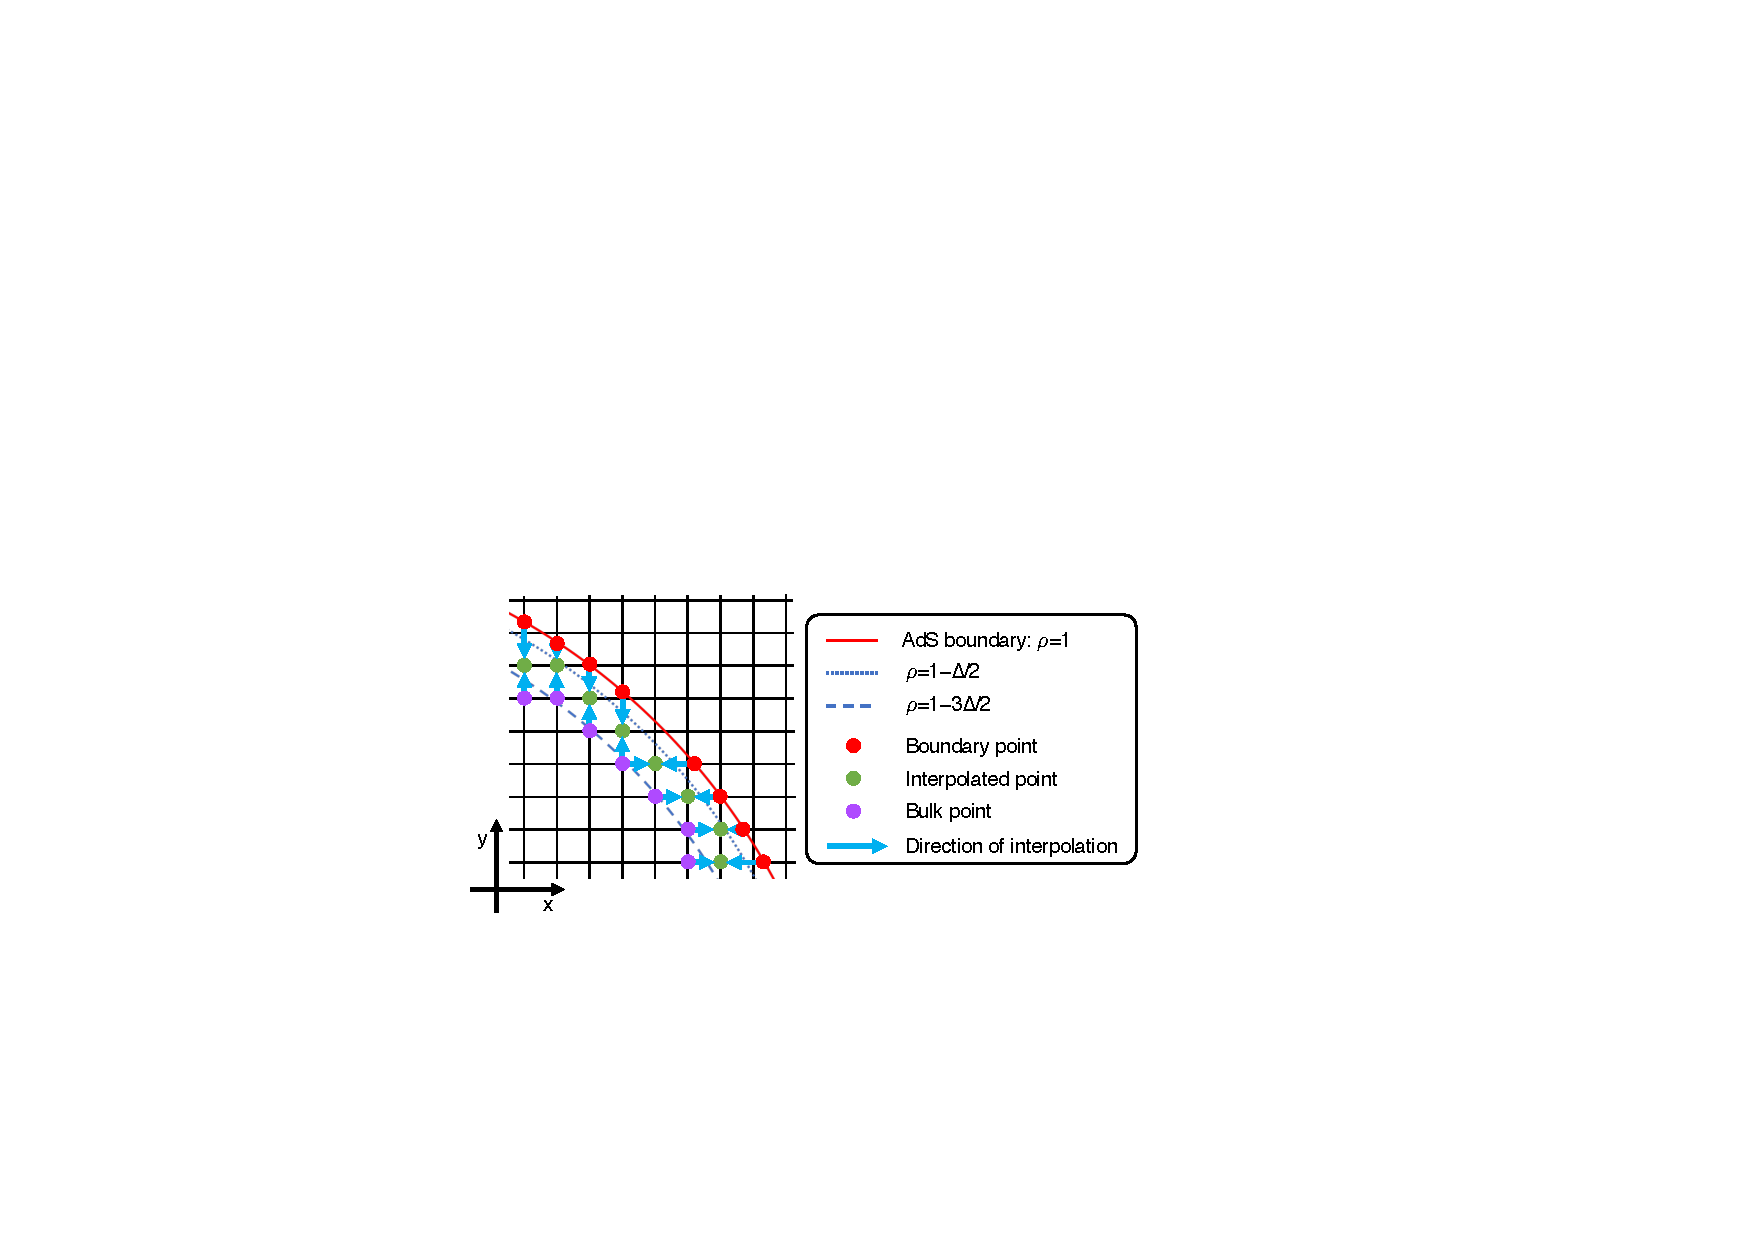
\includegraphics[width=6.0in,clip=true]{plots/lego_circle/Dirichlet_conditions.pdf}
\parbox{5.0in}{\caption{Visual description of implementation of Dirichlet boundary conditions through first order interpolation in a portion of a $z=const.$ surface for a grid with spatial refinement $\Delta$.
        }\label{fig:lego_circle_dirbc}}
\end{figure}

%The only complication comes from the fact that  $\rho=\sqrt{x^2+y^2+z^2}$ in Cartesian coordinates, so the AdS boundary $\rho=1$ generally does not lie on a Cartesian grid point. 
%We thus implement Dirichlet conditions as follows, see Figure~\ref{fig:lego_circle_dirbc}. 
%For any given evolution variable, we set its value at grid points with $\rho<1-\Delta/2$ (i.e., the green dots inside the blue dotted line in Figure~\ref{fig:lego_circle_dirbc}) by first order interpolation between the Dirichlet value at boundary points (red dots) and the value at the adjacent point further into the interior $\rho<1$ (purple dots). To identify the latter, we move along the Cartesian direction corresponding to the coordinate of the green dot with the largest absolute value. This direction is represented by light blue arrows. Notice that points with $\rho\geq1-\Delta/2$ are excised to avoid issues with quantities that would diverge (also analytically) at $\rho=1$.
%For any given evolution variable, we set its value at grid points that are at most one grid point away from $\rho=1$ by first order interpolation between the Dirichlet boundary value and the value at the closest point further into the interior $\rho<1$.  For the latter, we move along the Cartesian direction corresponding to the coordinate with the largest absolute value. 
%\textcolor{red}{A diagram here explaining which points are used and in which direction is necessary.}
%For any given evolution variable, we thus take its Dirichlet boundary condition at $\rho=1$ and its values at points further to the interior $\rho<1$ and use those to set its value, by first order interpolation, at grid points that are at most one grid point away from $\rho=1$.


Last but not least, time-symmetric initial data, sourced by a massless real scalar field, are obtained by solving the conformal decomposition of the Hamiltonian constraint \eqref{eq:hamconsfinal}. 
The solution to \eqref{eq:hamconsfinal} is computed, after second order finite discretization, through a full approximation storage (FAS) multigrid algorithm with v-cycling and Newton-Gauss-Seidel relaxation, built into the PAMR/AMRD libraries. We ensure that initial data satisfies the generalized harmonic constraints. See Appendix~\ref{sec:initdata} for more details and the complete choice of initial data.

\subsection{Apparent Horizon Finder and Excision}
\label{sec:AH_exc}

Once the solution is obtained at a certain time $t$, we can search for the position $R(\theta,\phi)$ of an apparent horizon (AH). We  use the following flow method in spherical coordinates $(\rho,\theta,\phi)$, obtained in the usual way from the Cartesian coordinates of the solution. We consider $n$ two-dimensional surfaces at constant, equally spaced, values of $\rho$ within a user-specified range between 0 and 1, and we pick the one with smallest $L^2$-norm of the outward null expansion. Let $\rho_0$ be the $\rho$ coordinate on this surface. 
Starting from the initial guess $R(\theta,\phi)=\rho_0$, for any $(\theta,\phi)\in [0,\pi)\times [0,2\pi)$ we find the solution to the equation
\begin{equation}
\label{eq:floweq}
\frac{dR(\theta,\phi)}{d s}=-\Theta(\rho,\theta,\phi)|_{\rho=R(\theta,\phi)},
\end{equation}
where $\Theta(\rho,\theta,\phi)|_{\rho=R(\theta,\phi)}$ is the outward null expansion of the two-dimensional surface given by $F(\rho,\theta,\phi)\equiv\rho-R(\theta,\phi)=0$. We iterate this process with starting point given by the solution $R(\theta,\phi)$ to \eqref{eq:floweq} found in the previous iteration. Assuming that the initial guess $\rho_0$ is not too distant from the position of the AH, the $R(\theta,\phi)$ is expected to progressively approach the AH after each iteration. 
This process stops when either the $L^2$-norm of $\Theta(\rho,\theta,\phi)|_{\rho=R(\theta,\phi)}$ is below some specified tolerance, i.e., $R(\theta,\phi)$ is sufficiently close to the AH, or the user-specified maximum number of iterations has been reached, i.e., either there is no AH at time $t$ or this method was not able to find it. 
%The latter typically occurs if we start from an initial guess $\rho_0$ which is not sufficiently close to the AH.

This AH finder is based on a $(\theta,\phi)$ grid\footnote{The grid on which the AH finder is executed is completely independent of the specifics of the Cartesian evolution grid given in Section~\ref{sec:numcauprob}.} with equal grid spacings $\Delta \theta=\Delta\phi=\Delta_{AH}$. The outward null expansion at grid points $(\theta,\phi)$ is obtained by first order interpolation in three dimensions from the values of the expansion at Cartesian grid points that surround $(\theta,\phi)$. These values are calculated from the definition of outward null expansion once the spacetime metric at time $t$ is known.
We observe that a $N_\theta\times N_\phi=9\times 17$ resolution is enough to find the AH in the simulations considered in Section~\ref{sec:results} in less than $10^{4}$ iterations. Since \eqref{eq:floweq} is a parabolic equation, the ``time'' step $\Delta s$ must be at least of order $\Delta_{AH}^2$ for stability. When using $n=10$ and an initial range for $\rho$ values between 0.1 and 0.5, as we do in our simulations, we find that the AH finder works effectively if $\Delta s$ takes much smaller values. Specifically, we set $\Delta s=10^{-4}$.

When an AH is found, we excise Cartesian grid points in an ellipsoid included in the AH and centred at the centre of the AH, in order to avoid the formation of geometric singularities in the computational domain.\footnote{This method is effective in removing singularities if the following common assumptions are valid on the spacetimes that we consider: (i) weak cosmic censorship is not violated, i.e., geometric singularities are contained inside a black hole event horizon, (ii) the AH at any time $t$ is contained in $t$-constant slices of the event horizon, (iii) the AH at any $t$ provides a sufficiently accurate approximation for $t$-constant slices of the event horizon.}
More specifically, the excision ellipsoid has Cartesian semi-axes, $a_x^{ex},a_y^{ex},a_z^{ex}$, determined by $a_x^{ex}=x_{AH}(1-\delta_{ex})$, where $x_{AH}$ is the $x$-coordinate value of the intersection between the AH and the $x$-axis, and similarly for $a_y^{ex}$ and $a_z^{ex}$. We set the excision buffer to $\delta_{ex}=0.4$. 
In our simulations, we assume that the characteristics of the equations of motion in the AH region flow towards the origin, although we do not compute the characteristics explicitly.\footnote{This is a reasonable assumption given the causal properties of a black hole. In fact, if this assumption were not true, we would see clear signs of constraint violations developing near the excision surface.} As a consequence, the solution at points inside the AH only evolves to affect points, at later times, that are further inside the AH. In other words, the information needed to solve the equations of motion on and outside the excision surface at a certain time is entirely contained in the numerical domain at previous times. This allows us to solve the equations of motion at the excision surface by employing one-sided stencils that do not reference points inside the excised region, with no need to impose conditions at the excision boundary. By construction, the excised surface is the same for all three time levels involved in the Newton-Gauss-Seidel relaxation for evolution variables at time $t$. Therefore, we only need to use the one-sided version of spatial stencils. 

It commonly occurs that the excised surface moves during evolution and previously excised points become unexcised. In this case, we initialize the value of newly unexcised points closest to the previous surface using  fourth order extrapolated values from adjacent exterior points along each Cartesian direction. We do so for any variable and at all three time levels of the hierarchy.
Finally, Kreiss-Oliger dissipation~\cite{kreiss1973methods} is essential to damp unphysical high-frequency noise that arise at excision grid boundaries; we use a typical dissipation parameter of $\epsilon_{KO}=0.35$.

%\medskip\hrule height 2pt %HB

\section{Results}\label{sec:results}

As a proof-of-principle, we evolve initial data that undergoes gravitational collapses within one light-crossing time, and follow the subsequent ring-down to the Schwarzschild-AdS solution.
%In this section we discuss the most evident features of the long-time evolution of time-symmetric initial data in the presence of a massless real scalar field with Gaussian profile, distorted along each Cartesian direction and centred at $x=y=z=0$:
The geometry of the initial slice is sourced by a massless real scalar field with a Gaussian profile, distorted along each Cartesian direction and centred at $x=y=z=0$ as follows:
\begin{eqnarray}
\label{eq:scaGaupro}
\bar{\varphi}|_{t=0}&=&A e^{-(\tilde{r}(x,y,z)/\Delta)^2},\\
\tilde{r}(x,y,z)&\equiv&\sqrt{ x^2(1-e_x^2)+ y^2(1-e_y^2)+ z^2(1-e_z^2)}. \nonumber
\end{eqnarray}
The amplitude of the profile is $A=0.55$ and  the eccentricities are $e_x=0.3, e_y=0.2, e_z=0.25$, so that the most prominent distortion is on the $(x,y)$-plane. The width of the Gaussian is $\Delta=0.2$. 
We choose the initial slice to be a moment of time symmetry, and the details of the time-symmetric initial data sourced by this matter field are collected in Appendix~\ref{sec:initdata}. 
As we see in that Appendix, the momentum constraint is trivially satisfied for this type of data, so only the Hamiltonian constraint needs to be solved. We evolve this initial data up to $t=31$ in units of AdS radius $L=1$ (approximately 20 light crossing times), well after the end of gravitational collapse and the resulting black hole formation. 
The initial data has zero total angular momentum 
%computed via the prescription in [CITE hep-th/9902121],
and angular momentum conservation [CITE arXiv:1211.6347v3 [gr-qc]] ensures that this is zero at all times. 
Therefore, we can expect the black hole to settle down to the Schwarzschild-AdS solution. However, for generic initial data with non-vanishing total angular momentum, this may not be the final state: \cite{Holzegel:2011uu} conjectured that Schwarzschild-AdS, or more generally Kerr-AdS, may suffer from a non-linear instability for generic perturbations.
%a rigorous proof for the uniqueness of Schwarzschild-AdS with the assumptions made in this initial data has not yet been obtained.\footnote{For example, in our setting, one could imagine that there exist asymptotically AdS spacetimes with zero angular momentum describing a rotating black hole whose angular momentum is compensated by the angular momentum of a scalar (or gravitational) cloud. However, such alternative configurations seem to be, if they exist, rather fine-tuned. It is thus highly unlikely that an arbitrary choice of initial conditions evolves to similar scenarios.}
We now will focus, separately, on the evolution of quantities defined in the bulk of the numerical grid and quantities defined on the AdS boundary.

%- Intro
%. long run 
%. completely asymmetric scalar field initial data
%. convergence of bulk and boundary quantities
%. preliminary conclusions about physical properties
%In this Section we present the details of a representative run starting from initial data with a completely asymmetric massless scalar scalar field. We will focus, separately, on quantities defined on the bulk of the numerical grid and quantities defined on the AdS boundary. We aim to show that these converge to their exact versions as we increase the grid resolution, and to draw some preliminary conclusions about physical properties of the solution, which will be analysed thoroughly in the future.



%-Collapse and Ringdown .time-symmetry .scalar field profile (amplitude, eccentricities, delta) . scalar field snapshots .relative Kretschmann approach Schw-AdS with a certain AdS mass .collapse in 0 bounces in a time of order $amp^2$ (consistent with Bizon-Rostorowski prediction for spherical symmetry) .cascade to the UV modes for scalar field but amplitude of scalar field is decreasing, so instability might .grid function convergence .iresall convergence

%- Boundary Stress-Energy Tensor .extrapolation technique .expression for components . analytic tracelessness .analytic conservation .convergence . tracelessness .conservation

\subsection{Collapse and ringdown}\label{sec:rescolring}

We describe here the evolution in the bulk: this  consists of an initial  short phase, in which the scalar field collapses and forms a black hole, and a long ringdown stage, in which the spacetime settles down to Schwarzschild-AdS. 

%Denoting the numerical value of any bulk quantity $f$ for the resolution with grid spacing $\Delta$ at grid point $p$ by $f_{\Delta}(p)$, our estimate for the solution error of $f_\Delta(p)$ is given by $\max(||\epsilon_\Delta(p)||_2,\Delta^3)$, where $\epsilon_\Delta(p)=\frac{1}{(3/2)^2-1} (f_{3\Delta/2}(p)-f_\Delta(p))$ is an approximation for the true solution error, $e_\Delta(p)$, motivated by the Richardson expansion \eqref{eq:Richexp}, and $||\cdot||_2$ denotes the $L^2$-norm.

\begin{figure}[!h]
        \centering
        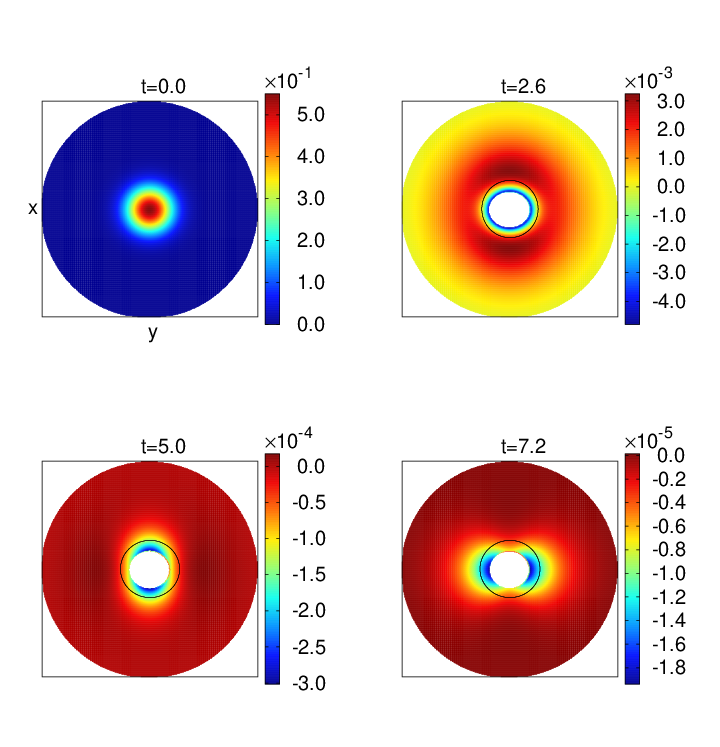
\includegraphics[width=5.2in,clip=true]{plots/bulkplots/L3/phi1/phi1_L3_snapshots_2by2.png}
\parbox{5.0in}{\caption{Snapshots of the scalar field profile $\bar{\varphi}$ on the $z=0$ slice in $(x,y)$ coordinates. In each plot, $x$ and $y$ are the horizontal and vertical axes, respectively, and the black square denotes the boundary of the numerical grid, i.e., $x=\pm 1$ and $y=\pm 1$. The external boundary of the coloured part is the AdS boundary $\rho=1$. The black ellipse denotes the approximate position of the AH. This is obtained as the $z=0$ slice of the ellipsoid with Cartesian semi-axes, $x_{AH},y_{AH},z_{AH}$, where $x_{AH}$ is the $x$-coordinate value of the intersection between the AH and the $x$-axis, and similarly for $y_{AH}$ and $z_{AH}$.
The internal boundary of the coloured region is the excision surface: we excise points inside an ellipsoid whose semi-axes, $a_x^{ex},a_y^{ex},a_z^{ex}$, are given by $a_x^{ex}=x_{AH}(1-\delta_{ex})$, and similarly for $a_y^{ex}$ and $a_z^{ex}$. We use the value $\delta_{ex}=0.4$ for the excision buffer. (Highest resolution: $N_x=N_y=N_z=325$.)
        }\label{fig:snapshotsscalarfield}}
\end{figure}

Figure \ref{fig:snapshotsscalarfield} shows four representative times of the scalar field variable's profile $\bar{\varphi}$ on the equatorial plane $z=0$ for the highest resolution grid with $N_x=N_y=N_z=325$ grid points along each Cartesian direction. Notice that, in all of these, $\bar{\varphi}=0$ at the AdS boundary as required by the Dirichlet boundary condition. At $t=0$, the asymmetry of the initial Gaussian profile is too small to be visible. At the beginning of evolution, we see that the scalar field starts spreading towards the AdS boundary but, before reaching it, a significant portion  is attracted back towards the origin and forms an apparent horizon (AH).  This occurs at $t=0.331$ in the highest resolution simulation. The rest of the scalar field remains outside the black hole, where it keeps bouncing back and forth the AdS boundary and it is gradually absorbed.
The asymmetry on the $(x,y)$-plane is clearly visible at $t=2.6$, where the scalar field is stretched along the $x$-direction and squeezed along the $y$-direction. The elongation changes its direction multiple times during the evolution, as shown in the next two plots: it is along the $y$-axis at $t=5.0$ and again along the $x$-axis at $t=7.2$.  However, the elongation, and hence the lack of spherical symmetry,  decreases exponentially in time as the scalar field is absorbed by the black hole. 
%Furthermore, we see that the largest part of the scalar field progressively disappears from the exterior part of the spacetime by entering the apparent horizon, hence the amplitude of the scalar field decreases. 
%In fact, we see that the scalar field is decaying exponentially in time. 
At later times, $t\simeq 9$, the value of the scalar field becomes consistent with 0 up to solution error\footnote{We estimate the solution error  by comparing $\bar{\varphi}$ at different resolutions.} and the spacetime settles down to a Schwarzschild-AdS black hole spacetime with mass $M=0.403$.

\begin{figure}[!h]
        \centering
        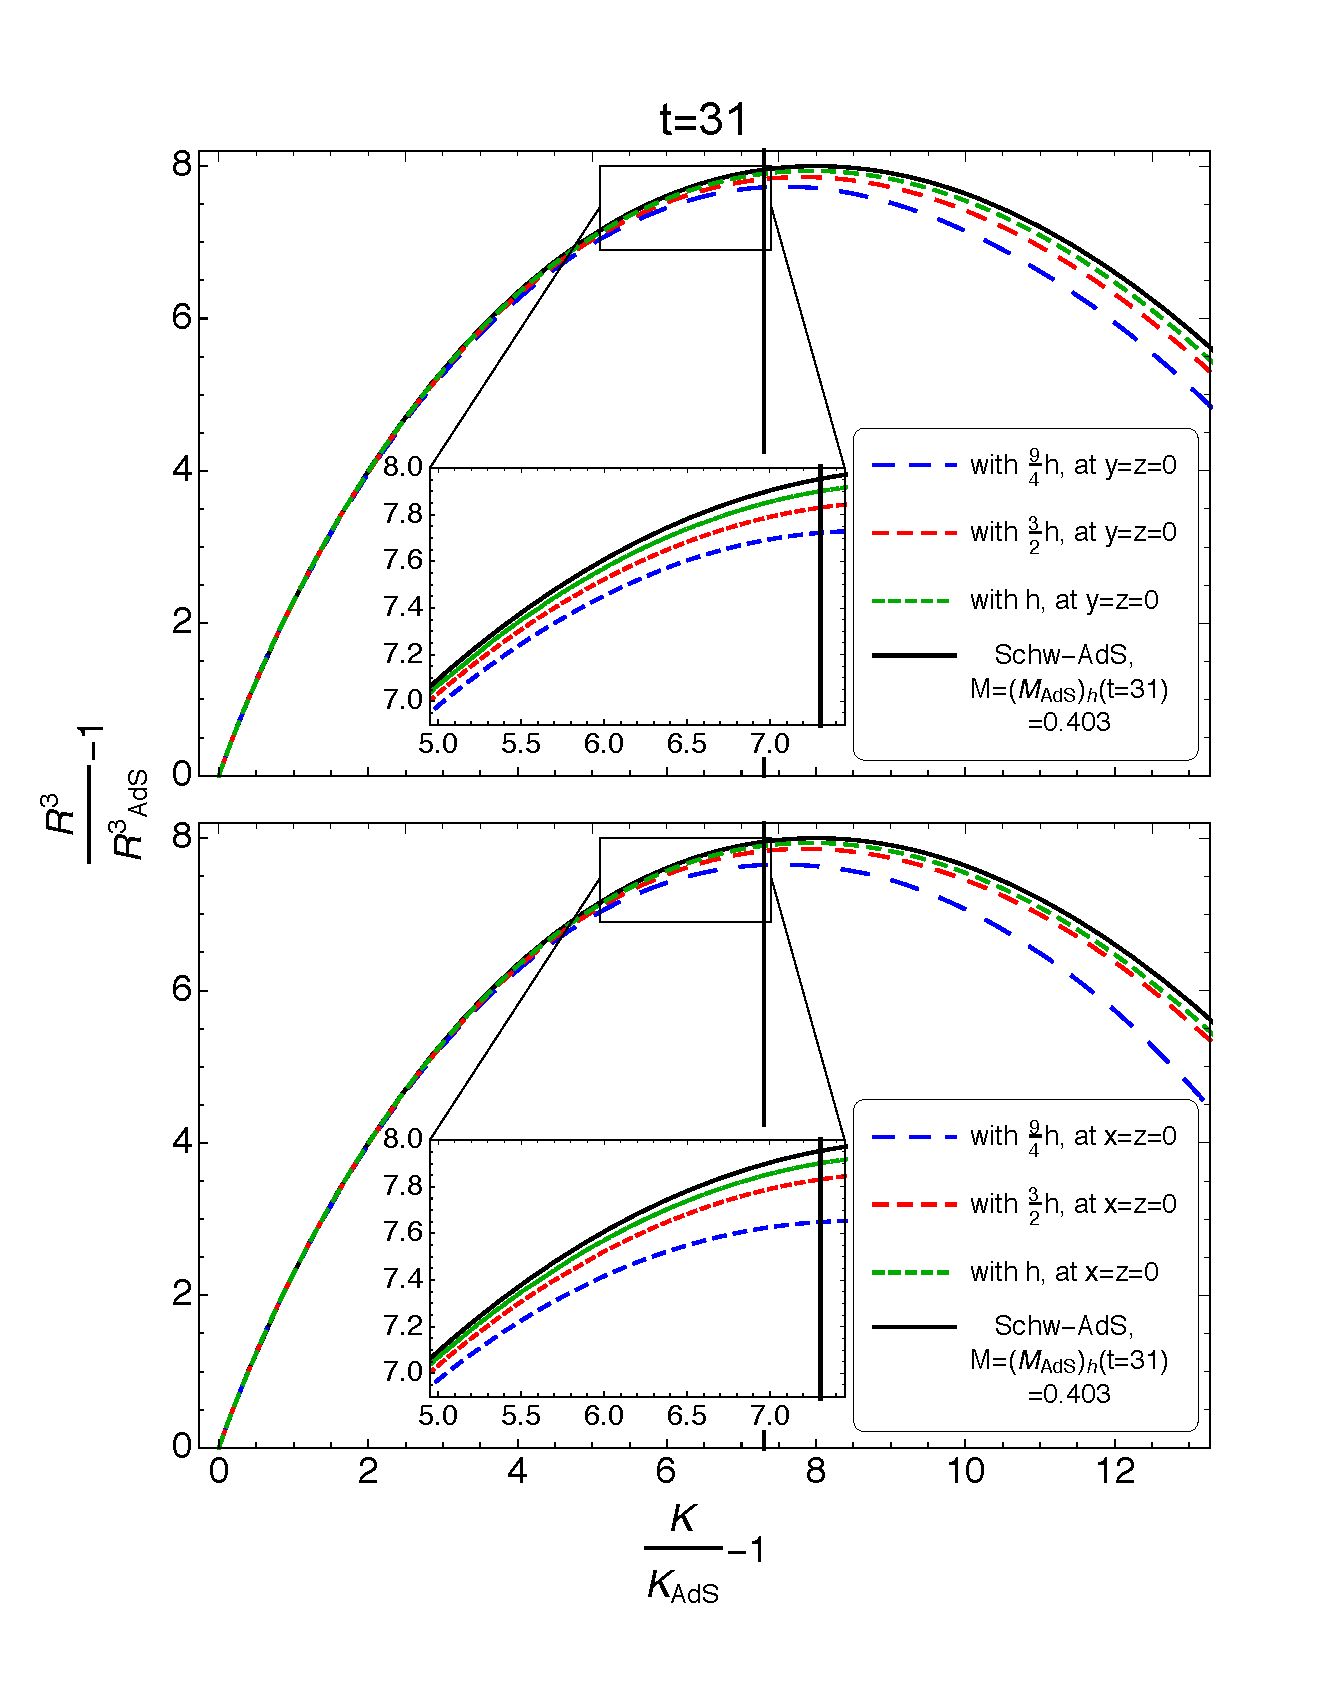
\includegraphics[width=5.25in,clip=true]{plots/bulkplots/compare_res/relriemanncube-relkretsch/combined_withzoom_fullplotrelRieCubeofrelkretschallres.pdf}
\parbox{5.0in}{\caption{Riemann cube scalar relative to $AdS_4$, $\frac{R^3}{R^3_{AdS}}-1$, as a function of Kretschmann scalar relative to $AdS_4$, $\frac{K}{K_{AdS}}-1$, for different resolutions at the last time step of the simulations, $t=31$, compared with the Schwarzschild-AdS case with mass given by $(M)_h=0.403$ (in units of AdS radius $L=1$), i.e., the value of $M$ (see eq. \eqref{eq:AdSmasscalc}) for the resolution with grid spacing $h$. The black vertical line denotes the value of $\frac{K}{K_{AdS}}-1$ at the horizon of Schwarzschild-AdS. Relative Kretschmann increases as we move closer to the origin of the spacetime. Top panel: numerical curves are obtained from grid points on the $x$ axis (i.e., $y=z=0$). Bottom panel: numerical curves are obtained from grid points on the $y$ axis (i.e., $x=z=0$). The asymmetry cannot be distinguished by eye.
        }\label{fig:relRiemanncube-relKretschmann-comparison-SchwAdS}}
\end{figure}

%\begin{figure}[!h]
%        \centering
%        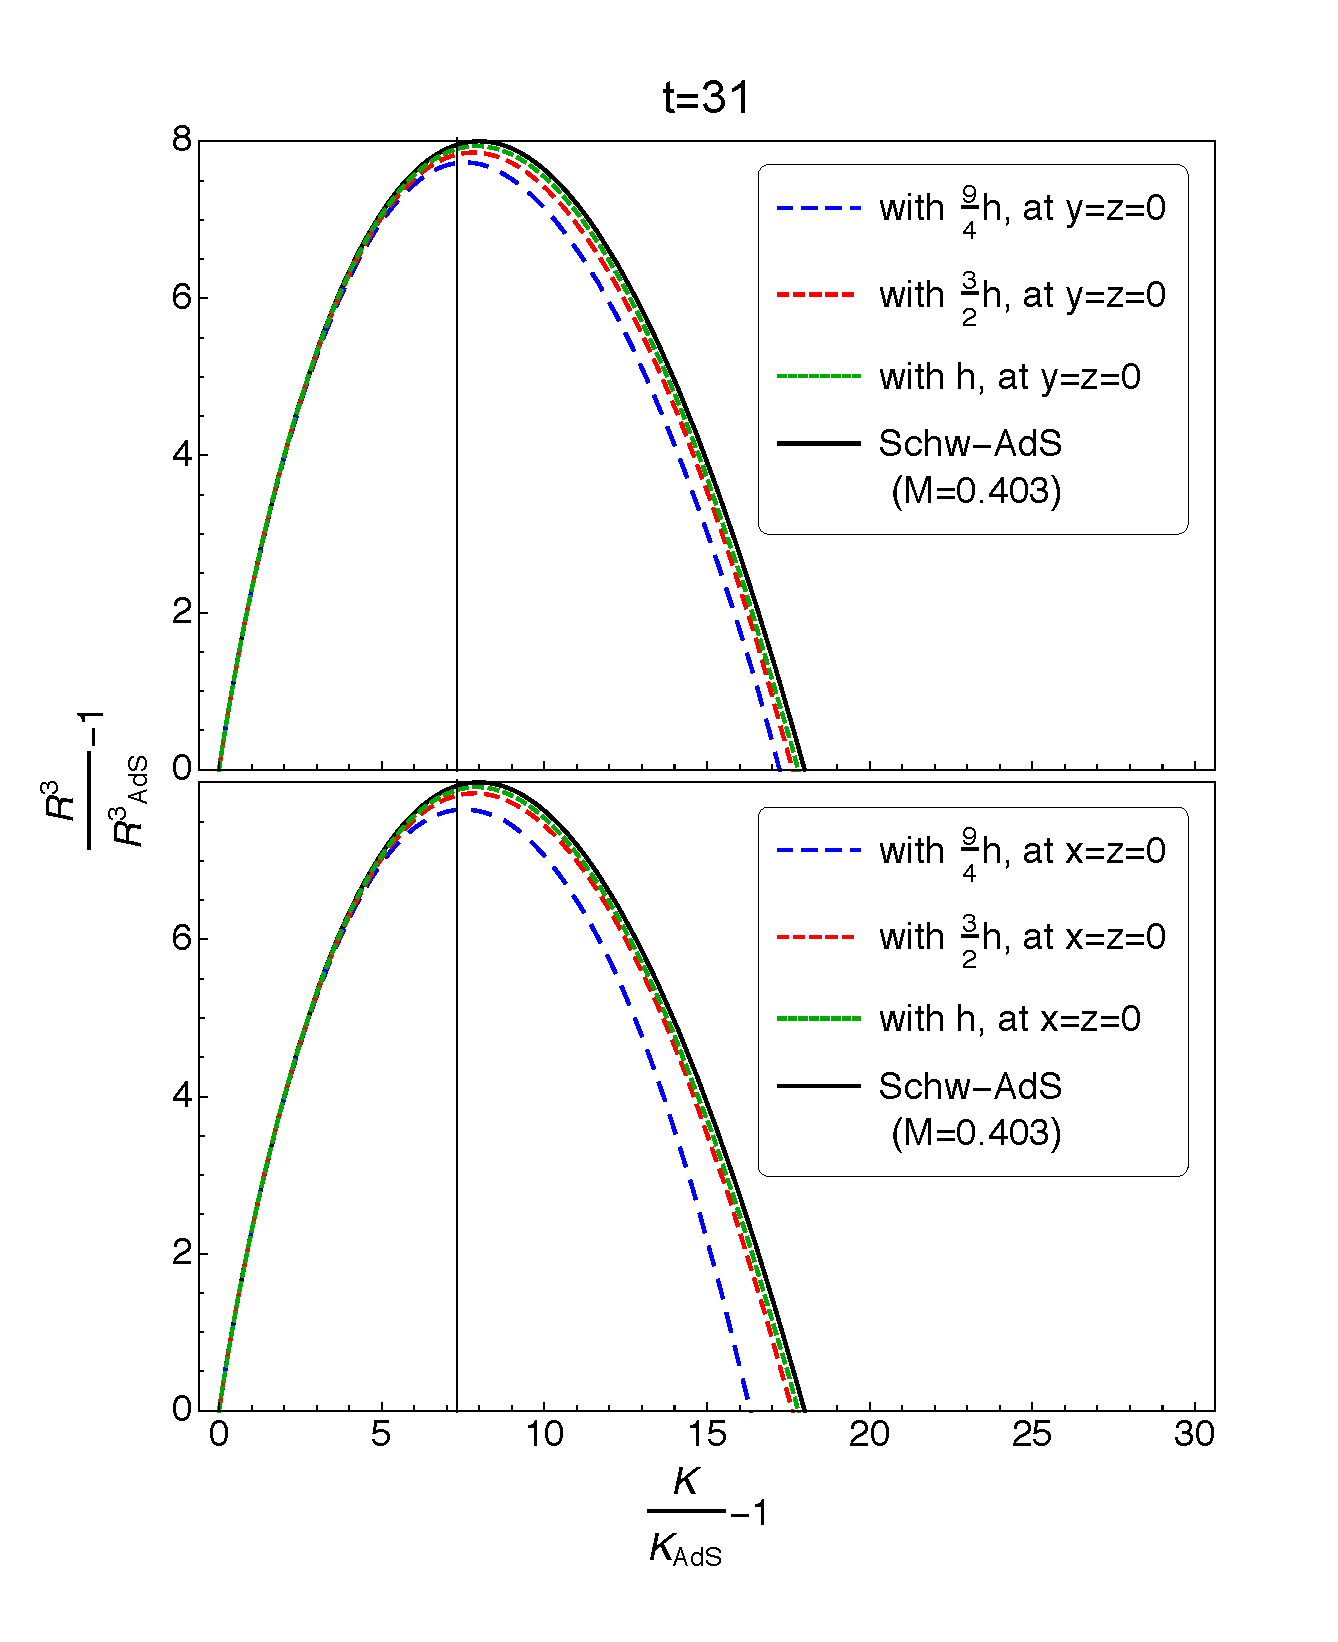
\includegraphics[width=5.0in,clip=true]{plots/bulkplots/compare_res/relriemanncube-relkretsch/option2_combinedplotrelRieCubeofrelkretschallres.pdf}
%\parbox{5.0in}{\caption{Riemann cube scalar relative to $AdS_4$, $\frac{R^3}{R^3_{AdS}}-1$, as a function of Kretschmann scalar relative to $AdS_4$, $\frac{K}{K_{AdS}}-1$, for different resolutions at the last time step of the simulations, $t=31$, compared with the Schwarzschild-AdS case with mass given by the value of $M_{AdS}$ at that time. Top panel: plot obtained using values on the $x$ axis (i.e., $y=z=0$). Bottom panel: plot obtained using values on the $y$ axis (i.e., $x=z=0$).
%        }\label{fig:relRiemanncube-relKretschmann-comparison-SchwAdS}}
%\end{figure}


%This can be seen explicitly in Figure \ref{fig:relRiemanncube-relKretschmann-comparison-SchwAdS}, in which we compare the numerical solution at the end of our simulations, $t=31$, to the Schwarzschild-AdS metric with mass $(M_{AdS})_h(t=31)=0.403$ (in units of AdS radius $L=1$), namely the highest resolution value of $M_{AdS}$ (given by equation \eqref{eq:AdSmasscalc}) at $t=31$, as follows. 
The late-time solution is close to Schwarzschild-AdS, which can be seen explicitly in Figure \ref{fig:relRiemanncube-relKretschmann-comparison-SchwAdS}.
Here, we compare the numerical solution at the last time slice, i.e., $t=31$, to the Schwarzschild-AdS metric with conserved mass obtained from our highest resolution run ($M=0.403$).
This comparison is achieved with the following procedure.
First, we compute the Riemann cube scalar $R^3=R_{\mu\nu\rho\sigma}R^{\rho\sigma\gamma\delta}R_{\gamma\delta}^{\;\;\;\;\mu\nu}$, and the Kretschmann scalar $K=R_{\mu\nu\rho\sigma}R^{\mu\nu\rho\sigma}$ for our numerical solution at the last time slice. 
Second, we compute the corresponding values, $R^3_{AdS}$ and $K_{AdS}$, in pure $AdS_4$.
We then use all four quantities to show the relative Riemann scalar $\frac{R^3}{R^3_{AdS}}-1$ as a function of the Kretschmann scalar $\frac{K}{K_{AdS}}-1$ for the Schwarzschild-AdS spacetime, shown as the black line in Figure \ref{fig:relRiemanncube-relKretschmann-comparison-SchwAdS}. 
We do the same for the numerical solution for different resolutions at grid points along the $x$ axis ($y=z=0$ coloured lines of top panel) and the $y$ axis ($x=z=0$ coloured lines of bottom panel). 

The black vertical lines in Figure \ref{fig:relRiemanncube-relKretschmann-comparison-SchwAdS} denotes the value of $\frac{K}{K_{AdS}}-1$ at the horizon of Schwarzschild-AdS. 
Notice that $\frac{K}{K_{AdS}}-1=0$ at the AdS boundary by construction, so going to larger values of $\frac{K}{K_{AdS}}-1$ is equivalent to moving towards the centre of the grid.
Therefore the black vertical lines give an indication of the position of the AH relative to the AdS boundary.
The two panels of Figure \ref{fig:relRiemanncube-relKretschmann-comparison-SchwAdS} indicate that, sufficiently close to the AdS boundary, the curvature of the numerical solution is almost identical to Schwarzschild-AdS. For clarity, this is shown using only values of the Riemann cube and Kretschmann scalars along the $x$ and $y$ axes, but we verified this for values from the entire grid. 
At any given resolution, the numerical curvature starts to differ from their Schwarzschild-AdS values as we get close to the AH. 
%(and it diverges strongly at values of $\frac{K}{K_{AdS}}-1$ corresponding to positions very close to the excision surface, as expected but not shown in the figure). 
%However, the higher the resolution the closer we get to Schwarzschild-AdS even inside the AH.
%Finally, we notice that for low resolutions a persistent asymmetry between the $x$ and $y$ axes is visible also at late times both outside and inside the horizon, but this disappears for high enough resolutions.
However, these differences converge away as resolution is increased.
Finally, although there is an asymmetry at any given resolution between the $x$ and $y$ axes even at this last time slice, this late-time asymmetry also converges away as resolution is increased.

\subsection{Boundary scalar field and stress-energy tensor}
\label{sec:resbouset}

In this section we consider the evolution of quantities on the $\mathbb{R} \times S^2$ boundary at $\rho=1$, defined in Section~\ref{sec:bouset2}. 
These quantities are obtained via third order extrapolation from points in the interior, with the only exception of the $t=0$ plot of Figure \ref{fig:snapshotsbdyphi}, which is computed analytically from the initial distorted Gaussian profile \eqref{eq:scaGaupro}.
%as extrapolation would give values smaller than the solution error of the function. 

We start by noting that the numerical values for the total mass $M$ in AdS, obtained from equation \eqref{eq:AdSmasscalc}, are approximately constant during the evolution, as expected by mass conservation [CITE arXiv:1211.6347v3 [gr-qc]]. More precisely, a small drift of  the total mass  is observed numerically, however this becomes smaller as we increase the resolution and it is consistent with zero within our error estimate for boundary quantities that we will discuss shortly.
%given by the $L^2$-norm of the deviation from the theoretical zero value of $\langle trT\rangle_{CFT}$ (red line of Figure \ref{fig:fullplotfillregttraceanisotropyenergydensityminusschwmaxminusminbdyenergydensity.pdf}).

\begin{figure}[!h]
        \centering
        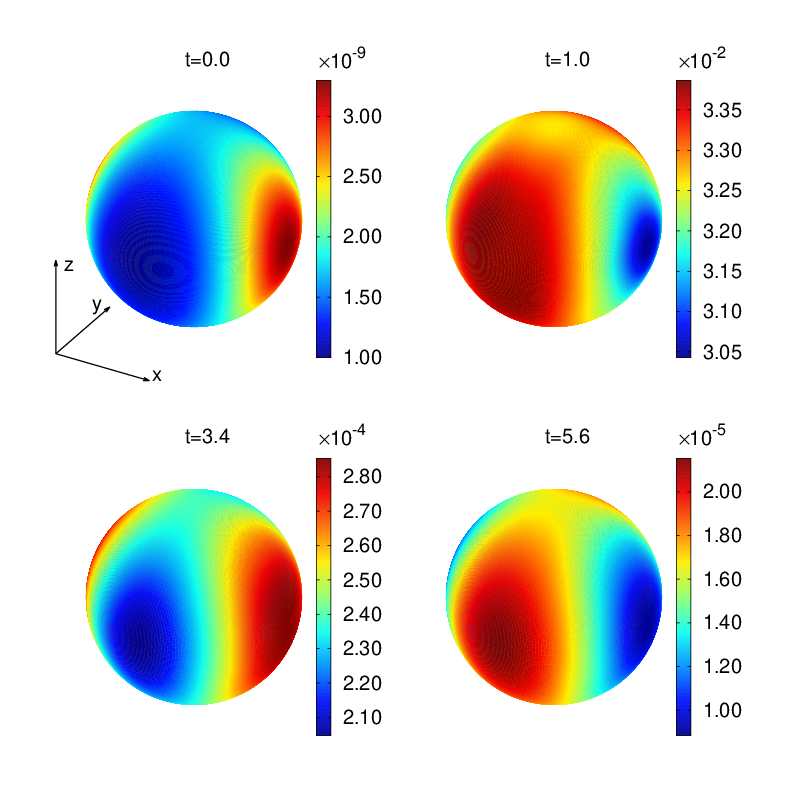
\includegraphics[width=5.0in,clip=true]{plots/bdyplots/L3/bdyphi/sphereplots_bdyphi_L3_2by2.png}
\parbox{5.0in}{\caption{
%Snapshots of the expectation value of the scalar field of the boundary CFT, $\langle \varphi\rangle_{CFT}$. 
Snapshots of the leading-order coefficient $\bar{\varphi}_{(1)}$ in the near-boundary expansion of the bulk scalar field. 
The first snapshot is obtained analytically from the initial scalar field profile. The remaining three are obtained by third order extrapolation and subsequent smoothening via a low-pass filter with threshold frequency $\omega=0.5$. (Highest resolution: $N_x=N_y=N_z=325$.)
        }\label{fig:snapshotsbdyphi}}
\end{figure}

%Figure \ref{fig:snapshotsbdyphi} shows four snapshots of the expectation value of the scalar operator $\langle \varphi\rangle_{CFT}$ of the boundary CFT.
Figure \ref{fig:snapshotsbdyphi} shows four snapshots of the leading-order coefficient $\bar{\varphi}_{(1)}$ in the near-boundary expansion of the bulk scalar field given in \eqref{eqn:qexp}.
Unlike the $z=0$ slice snapshots of Figure \ref{fig:snapshotsscalarfield}, these plots of the boundary $\mathbb{R}\times S^2$ encode the asymmetry in all three Cartesian directions in the bulk, as they appear on the boundary at $\rho = \sqrt{x^2+y^2+z^2}=1$. 
In fact, the asymmetry of the initial data is already visible at $t=0$, where the different values of eccentricities along the three Cartesian direction (largest along $x$ and smallest along $y$) are evident in this plot. At this time, the boundary scalar field is overall very small, which is expected since the initial $\bar{\varphi}$, given by \eqref{eq:scaGaupro}, is localised near $\rho=0$.
Notice from Figure \ref{fig:snapshotsbdyphi} that the asymmetry changes axes during evolution, but interestingly it is always strongest along $x$ and weakest along $y$ or vice-versa. Furthermore, a direct comparison with Figure \ref{fig:snapshotsscalarfield} shows that the features present at a certain $t$ at the boundary take approximately $\pi/2\simeq1.6$ to reach the interior of the bulk, i.e., about a light-crossing time, as expected. At later times, mirroring the evolution in the bulk, $\bar{\varphi}_{(1)}$ decays exponentially in time as the spacetime settles down to Schwarzschild-AdS.

\begin{figure}[!h]
        \centering
        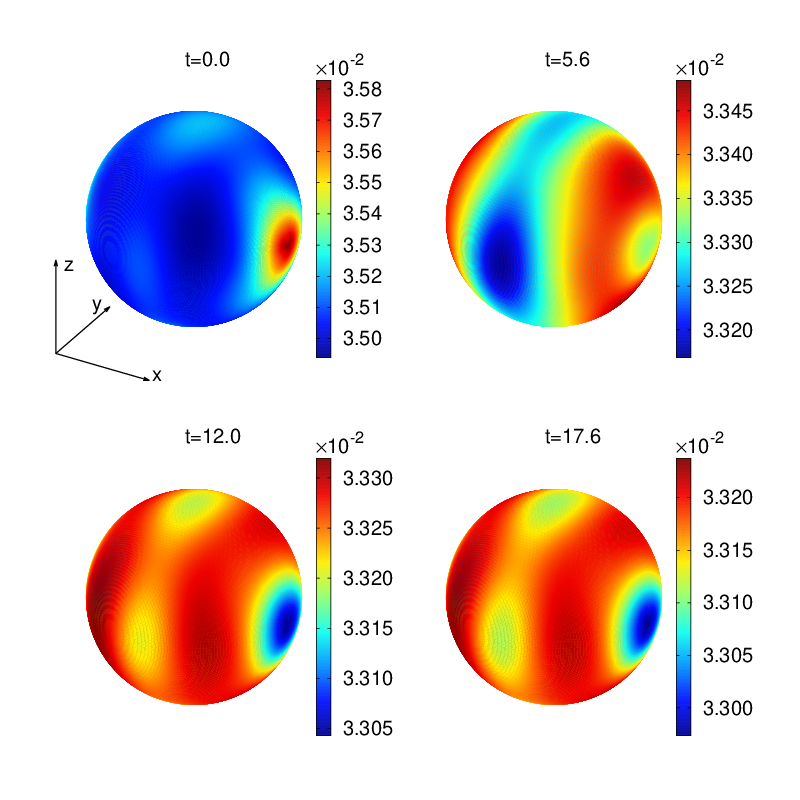
\includegraphics[width=5.0in,clip=true]{plots/bdyplots/L3/bdyenergydensity/sphereplots_bdyenergydensity_L3_2by2.png}
\parbox{5.0in}{\caption{Snapshots of energy density $\epsilon$ at the boundary, obtained by third order extrapolation and smoothened via a low-pass filter with threshold frequency $\omega=0.25$. The scale of each snapshot has fixed interval length centred at the mean value of  $\epsilon$ at the corresponding evolution time to make the approach to a uniform configuration more visible. (Highest resolution: $N_x=N_y=N_z=325$.)
        }\label{fig:snapshotsenergydensity}}
\end{figure}

Figure \ref{fig:snapshotsenergydensity} displays the energy density $\epsilon$ of the boundary CFT.
At $t=0$ this is strongly asymmetric along the $x$-direction, as expected from the shape of the initial scalar field \eqref{eq:scaGaupro}. 
After that, $\epsilon$ undergoes a phase of strong evolution with several changes of elongation axes, sampled at $t=5.6$ and terminating at approximately $t=7.2$. From that time onwards, $\epsilon$ settles down to a uniform configuration, as appropriate for the Schwarzschild-AdS case. Approach to uniformity is emphasized by using colour scales with fixed interval length, centred at the mean value of $\epsilon$ at the corresponding evolution time.


\begin{figure}[!h]
        \centering
        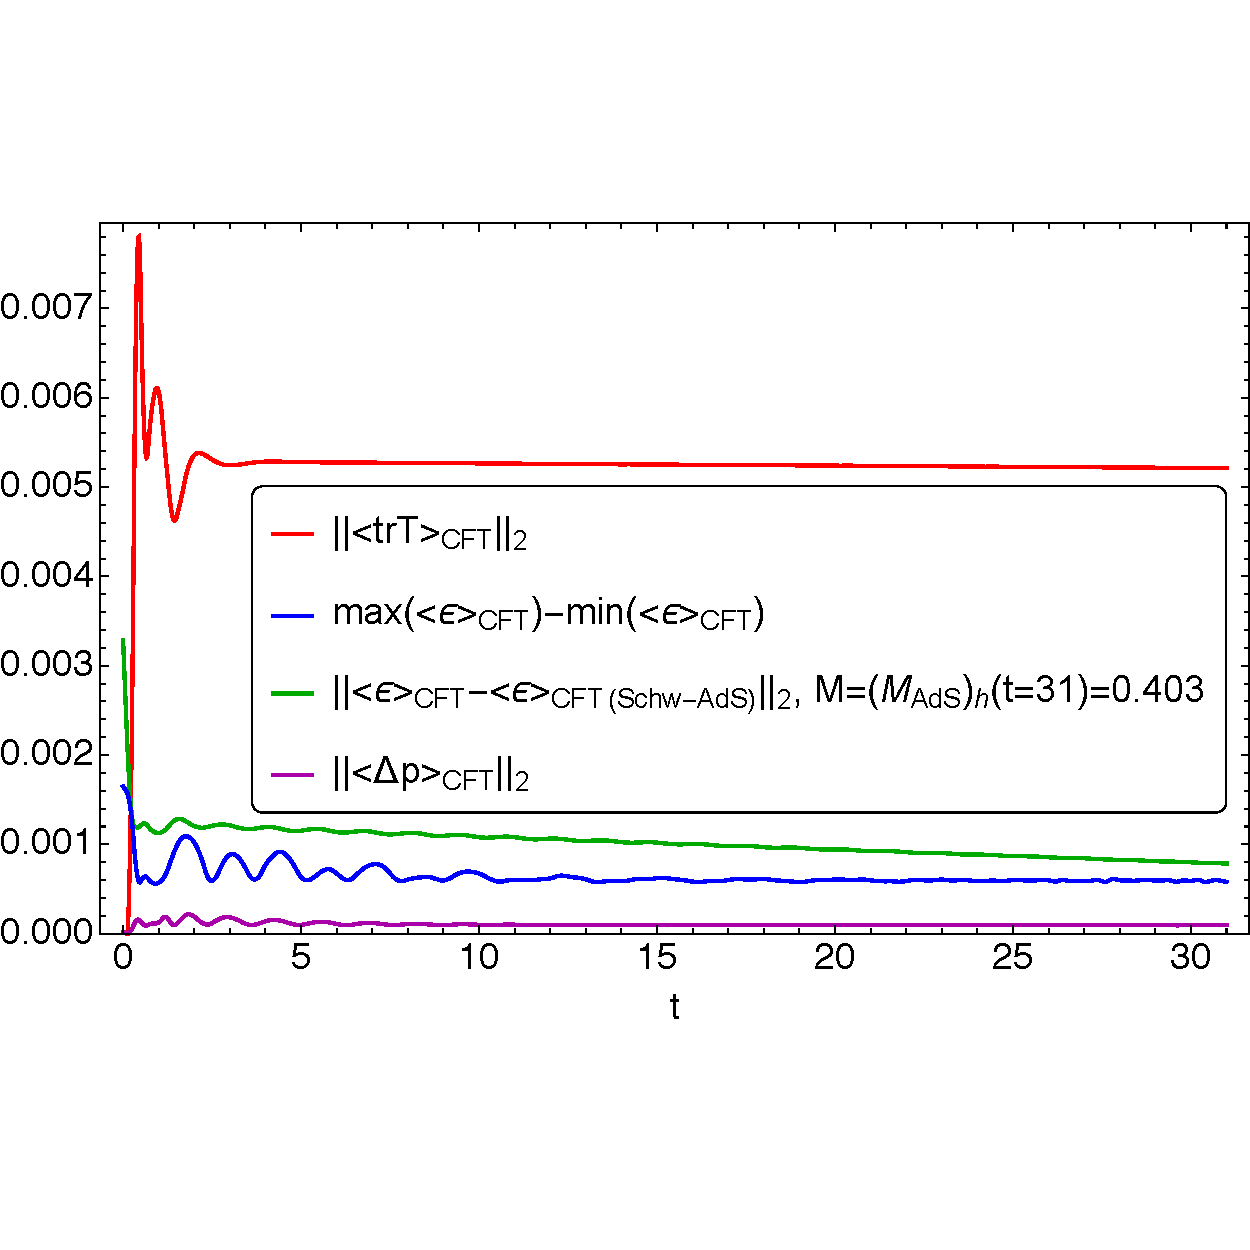
\includegraphics[width=5.0in,clip=true]{plots/timeseries/L2-norm_trace_anisotropy_energydensityminusschw_maxminusminenergydensity/fullplotfillregttraceanisotropyenergydensityminusschwmaxminusminbdyenergydensity_L3.pdf}
\parbox{5.0in}{\caption{Comparison of boundary quantities with error estimate given by the deviation of the $L^2$-norm of $\langle \text{tr}T\rangle_{CFT}$ from its predicted zero value for the 2+1 CFT (red line). We consider the following boundary quantities: difference between maximum and minimum of boundary energy density $\epsilon$ (blue line), $L^2$-norm of difference between $\epsilon$ and the Schwarzschild-AdS value $\epsilon_{Schw-AdS}=\frac{M}{4\pi}$ (green line), with Schwarzschild mass $M=(M)_h=0.403$ (i.e., the value of $M$ for the resolution with grid spacing $h$), $L^2$-norm of boundary anistropy $\Delta p$ (magenta line). This plot is obtained from the data of the highest resolution run ($N_x=N_y=N_z=325$), but at any resolution these quantities exhibit the same hierarchy, although at different scales. Boundary quantities are computed by third order extrapolation.
        }\label{fig:fullplotfillregttraceanisotropyenergydensityminusschwmaxminusminbdyenergydensity.pdf}}
\end{figure}

More information about the energy density of the boundary field theory can be deduced from Figure \ref{fig:fullplotfillregttraceanisotropyenergydensityminusschwmaxminusminbdyenergydensity.pdf}. 
The trace $\langle \text{tr}T\rangle_{CFT}$ vanishes for a conformal field theory in 2 +1 dimensions, which is the case for our $\mathbb{R} \times S^2$ boundary.
In Section~\ref{sec:bouset2}, we had spelled out how this trace, in our scheme, is tied to how well we are solving the Einstein field equations.
We thus use the $L^2$-norm of the numerical values of $\langle \text{tr}T\rangle_{CFT}$ (red line) as an error estimate for boundary quantities. We compare this error with the difference between maximum and minimum of $\epsilon$ (blue line), the $L^2$-norm of the difference between $\epsilon$ and its Schwarzschild-AdS value $\epsilon_{Schw-AdS}=\frac{M}{4\pi}$ (green line), with $M=(M)_h=0.403$, i.e., the highest resolution value of $M_{AdS}$, and the $L^2$-norm of $\Delta p$ (magenta line). We compute these quantities from the data of the highest resolution simulation (i.e., $N_x=N_y=N_z=325$), but at any resolution the hierarchy is the same, although it appears at different scales.
If we exclude very early times, we see that $\max(\epsilon)-\min(\epsilon)$ is consistent with 0, which confirms that the energy density becomes uniform in time.
We also see that $||\epsilon-\epsilon_{Schw-AdS}||_2$ is consistent with 0 and decreasing in time, which shows that the energy density settles down to $\epsilon_{Schw-AdS}$, as expected.
Finally, $||\Delta p||_2$ is consistent with 0, as appropriate for the boundary anistropy of Schwarzschild-AdS.




\section{Discussion}\label{sec:Discussion}

We have presented the first proof-of-principle Cauchy evolution of an asymptotically AdS spacetime determined by the Einstein-Klein-Gordon equations with no symmetry assumptions. Stability of the numerical scheme is achieved through the gauge choice \eqref{eqn:target_gauge_txyz} near the AdS boundary. The reliability of the scheme has been tested and a brief analysis of the numerical solution for stationary initial data with completely asymmetric Gaussian massless scalar field has been provided.

We observe the collapse of the scalar field into a black hole and the subsequent ringdown to a Schwarzschild-AdS spacetime, in both bulk and boundary quantities.
Deviations from Schwarzschild-AdS at late times are consistent with zero within estimates of the numerical error. 
At very late times, the spatial profiles of these small deviations appear to cascade towards higher harmonics.
Even though these deviations are consistent with our error estimates, they may nevertheless trigger a non-linear instability that can only be revealed by evolving for longer times.\footnote{Schwarzschild-AdS has been shown to be stable under spherically symmetric deformations \cite{Holzegel:2011uu}.} 
It will be interesting to conduct a detailed analysis by decomposing the scalar field profile into spherical harmonics and showing that the radial part is non-vanishing near the boundary for a very long time. 
We leave this for future studies.

In this work we limited ourselves to $d=4$ spacetime dimensions, but the calculation outlined in Section~\ref{sec:gauge_choice} would be almost identical if we were to study Cartesian evolution of asymptotically AdS spacetimes in any $d\geq4$ dimensions. In particular, the stable gauge found with this method would be the same up to a numerical factor. 
Interestingly, a comparison between \eqref{eqn:target_gauge_txyz} and the corresponding result in [cite arXiv:1706.04199 [hep-th] ] (see eq. (S10) in that previous work) clearly suggests a trend for the expression of the stable gauge in $D+1$ dimensions for any number $D\geq1$ of spatial dimensions. If this trend were confirmed, repeating the calculation above would not be necessary when changing the value of $D$. 
Furthermore, we have applied the scheme presented here to cases with different types of matter fields, different types of global coordinates, and to coordinates on a Poincar\'{e} patch. 
For instance, in Appendix~\ref{sec:sphevvarboucon} we followed the prescription of Section~\ref{sec:pre_sta} to obtain the stable gauge also in spherical coordinates. 
In Appendix~\ref{sec:poincare}, we write down a gauge that stabilizes evolution on a Poincar\'e patch of AdS$_4$.
In other words, this framework makes numerical Cauchy evolution in asymptotically AdS spacetimes possible in full generality, with no need to impose symmetries.

We expect to be able to tackle several interesting problems in asymptotically AdS spacetimes using this Cauchy evolution scheme. The most direct application would be the study of gravitational collapse of a massless scalar field with zero angular momentum in $AdS_4$. This has been analyzed in spherical symmetry by [CITE Bizon-Rostworowski] and in axisymmetry by [Bantilan-Figueras-Kunesch], although the two studies probe different ranges for the amplitude of the scalar field, so a direct comparison cannot be made. Solving the evolution equations through our scheme, the details of the collapse could be analysed even further in full generality.

Other important applications
%, requiring only minor additions to the capabilities of the current code, 
include the study of binary black hole mergers and black hole instabilities in AdS. In particular, the evolution of superradiantly unstable (see [cite Brito, Cardoso, Pani] for a review on superradiance) initial data for a Kerr-AdS black hole spacetime was followed in [cite CHESLER,LOWE], without imposing symmetries, up to approximately 290 light-crossing times using a characteristic scheme [cite Chesler, Yaffe]. This showed a transition of the Kerr-AdS black hole to a rotating black hole with one helical Killing field consistent with a black resonator [cite Dias, Santos, Way]. Since black resonators are fastly rotating black holes with an ergo-region, they are also unstable to superradiance [cite  Hawking, Reall] [cite Green, Hollands, Ishibashi, Wald] hence a cascade to smaller and smaller resonators, potentially leading to a violation of the weak cosmic censorship conjecture, was suggested [cite Niehoff,Santos,Way]. The authors of [cite CHESLER,LOWE] see a second transition at late times that could be the beginning of such cascade but they do not evolve further as Adaptive Mesh Refinement (AMR) becomes crucial to resolve small structures in a reasonable amount of running time. A code such as the one presented here, having AMR capabilities already built in, could be successful in reaching later stages of the evolution and potentially addressing the question about the end-state of superradiant instability of Kerr-AdS.



\section*{Acknowledgements}
HB and PF are supported by the European Research Council Grant No. ERC-2014-StG 639022-NewNGR. PF is also supported by a Royal Society University Research Fellowship (Grant No. UF140319 and URF\textbackslash R\textbackslash 201026) and by a Royal Society Enhancement Award (Grant No. RGF\textbackslash EA\textbackslash 180260).  LR is supported by a QMUL PhD scholarship. We acknowledge the use of Athena at HPC Midlands+, which was funded by the EPSRC on 
grant EP/P020232/1, in this research, as part of the HPC Midlands+ consortium. This research also utilised Queen Mary's Apocrita HPC facility, supported by QMUL Research-IT. http://doi.org/10.5281/zenodo.438045.

\appendix
\setcounter{tocdepth}{1}
\numberwithin{equation}{section}
\section{Generalized Harmonic Formulation}
\label{sec:GHfor}

The generalized harmonic formulation of the Einstein equations is based on coordinates $x^\alpha$ that each satisfies a wave equation $\Box x^{\alpha}=H^\alpha$ with source functions $H^\alpha$.
As long as the constraint $0=C^\alpha \equiv H^\alpha-\Box x^\alpha$ is satisfied, we can then write the trace-reversed Einstein equations in $d$ dimensions with cosmological constant $\Lambda$
\begin{equation}
0=R_{\alpha\beta} - \frac{2\Lambda}{d-2} g_{\alpha\beta} - 8\pi\left( T_{\alpha\beta} - \frac{1}{d-2} {T^\gamma}_\gamma g_{\alpha\beta} \right)
\end{equation}
as
\begin{eqnarray}
0
&=& R_{\alpha\beta} - \nabla_{(\alpha} C_{\beta)} - \frac{2\Lambda}{d-2} g_{\alpha\beta} - 8\pi\left( T_{\alpha\beta} - \frac{1}{d-2} {T^\gamma}_\gamma g_{\alpha\beta} \right) \nonumber \\
&=& R_{\alpha\beta} - \nabla_{(\alpha} H_{\beta)} + \nabla_{(\alpha} \Box{x}_{\beta)} - \frac{2\Lambda}{d-2} g_{\alpha\beta} - 8\pi\left( T_{\alpha\beta} - \frac{1}{d-2} {T^\gamma}_\gamma g_{\alpha\beta} \right) \nonumber \\
&=& -\frac{1}{2} g^{\gamma\delta} g_{\alpha\beta,\gamma\delta} - g^{\gamma\delta}{}_{,(\alpha}g_{\beta)\gamma,\delta} - H_{(\alpha,\beta)} + H_\gamma \Gamma^\gamma{}_{\alpha\beta} \nonumber \\
&&- \Gamma^\gamma{}_{\alpha\delta}\Gamma^\delta{}_{\gamma\beta} - \frac{2\Lambda}{d-2} g_{\alpha\beta} - 8\pi\left( T_{\alpha\beta} - \frac{1}{d-2} {T^\gamma}_\gamma g_{\alpha\beta}\right) \,, \label{eqn:Eeqs} 
\end{eqnarray}
where the choice of $H_\alpha = g_{\alpha\beta} H^\beta$ fixes the gauge, $\Gamma^\alpha{}_{\beta\gamma}$ are the Christoffel symbols  associated to the spacetime metric $g_{\alpha\beta}$, and $T_{\alpha\beta}$ is the matter stress-energy tensor. 
To suppress constraint-violating solutions that do not satisfy $C_\alpha=0$, we supplement \eqref{eqn:Eeqs} with constraint-damping terms as introduced in~\cite{Gundlach:2005eh} and obtain our final form of the Einstein equations:
\begin{eqnarray}
\label{eqn:efe_gh_modified}
&-& \frac{1}{2} g^{\gamma \delta} g_{\alpha\beta, \gamma \delta} - 
{g^{\gamma\delta}}_{,(\alpha} g_{\beta) \gamma, \delta} - H_{(\alpha, \beta)} + H_\gamma {\Gamma^\gamma}_{\alpha\beta} \nonumber \\
&-& {\Gamma^\gamma}_{\delta \alpha} {\Gamma^\delta}_{\gamma \beta} - \kappa \left( 2 n_{(\alpha} C_{\beta)} - (1+P) g_{\alpha\beta} n^\gamma 
C_\gamma \right) \nonumber \\
&=&   \frac{2}{d-2} \Lambda g_{\alpha\beta} + 8\pi \left( T_{\alpha\beta} - 
\frac{1}{d-2} {T^\gamma}_\gamma g_{\alpha\beta} \right).
\end{eqnarray}

See, for example, CITE [arXiv:gr-qc/0407110] , [arXiv:1201.2132v3 [hep-th]] for more details. In our simulations we use the values $\kappa=-10$ and $P=-1$.\footnote{CITE [arXiv:1201.2132v3 [hep-th]] mentions that it is important to use $P$ close to $-1$, while the value of $\kappa$ is not too important to achieve effective constraint damping.}

In this work, we are interested in the case where matter fields are given by a single massless real scalar field $\varphi$, hence the stress-energy tensor reads
\begin{equation}
\label{eq:KHmomtens}
T_{\alpha\beta}=\partial_\alpha \varphi \partial_\beta \varphi - g_{\alpha\beta} \frac{1}{2} g^{\gamma\delta} \partial_{\gamma} \varphi \partial_{\delta} \varphi,
\end{equation}
and $\varphi$ is coupled to $g_{\alpha\beta}$ through the Klein-Gordon equation \eqref{eqn:eoms2}, which we write here for completeness in terms of partial derivatives w.r.t. the chosen set of coordinates:
\begin{equation}\label{eqn:eoms2cart}
g^{\alpha\beta} \partial_{\alpha} \partial_{\beta} \varphi -g^{\alpha\beta} \Gamma^{\gamma}{}_{\beta\alpha}\partial_\gamma\varphi= 0.
\end{equation}











\section{Boundary Prescription in Spherical Coordinates}\label{sec:sphevvarboucon}

Although spherical coordinates $x^\alpha=(t,\rho,\theta,\phi)$ are not suitable for numerically evolving points near the origin (see discussion in Section~\ref{sec:numcauprob}), they are convenient to extract the physics of the CFT at the AdS boundary $\rho=1$, since they are adapted to the boundary topology $\mathbb{R}\times S^2$.
In this section we apply the prescription outlined in Section~\ref{sec:pre_sta} to the case of asymptotically AdS spacetimes in 4 dimensions in spherical coordinates. Similarly to the Cartesian case, we first define the spherical coordinate version of the evolution variables $(\bar{g}_{\alpha\beta},\bar{\varphi},\bar{H}_\alpha)$. We also write down the transformations between these variables and their Cartesian version, \eqref{eq:gbarcart}, \eqref{eq:phibarcart}, \eqref{eq:soufunb}. Then, we obtain the stable gauge in spherical coordinates by following the steps introduced in Section~\ref{sec:gauge_choice}. We compare this with a different potentially stable gauge that can be inferred from the one used in~\cite{Bantilan:2012vu}. Finally, we show that tracelessness and conservation of the boundary stress-energy tensor $\langle T_{ab}\rangle_{CFT}$, defined in Section~\ref{sec:bouset2}, is a consequence of the lowest order of the Einstein equations, provided that the leading order of the generalized harmonic constraints is satisfied.\footnote{In fact, tracelessness was already proved in Section~\ref{sec:bouset2} by converting Cartesian variables into spherical ones. We prove it again in this section employing only spherical coordinates.}


%Here we apply the prescription of Section~\ref{subsec:cartevvarboucon} to the case of asymptotically AdS spacetimes in spherical coordinates $x^\alpha=(t,\rho,\theta,\phi)$, in order to construct the spherical coordinate version of the Cartesian evolution variables $(\bar{g}_{\mu\nu},\bar{\varphi},\bar{H}_\mu)$. We also write down the transformations between these two sets of variables in different coordinates.

\subsection{Evolution Variables and Boundary conditions}

We remind the reader that new evolution variables are defined in order to apply the boundary conditions found in Section~\ref{subsec:asyAdS} as simple Dirichlet conditions at the AdS boundary $\rho=1$. In the same way as in the Cartesian coordinate case, the metric evolution variables in spherical coordinates $\bar{g}_{\alpha\beta}$ are defined by (i) considering the deviation from pure AdS tensor $h_{\alpha\beta}=g_{\alpha\beta}-\hat{g}_{\alpha\beta}$ in spherical coordinates, and (ii) stripping $h_{\alpha\beta}$ of as many factors of $(1-\rho^2)$ as needed so that they fall off linearly in $(1-\rho)$ near the AdS boundary at $\rho=1$.

The boundary conditions on $h_{\alpha\beta}$ \eqref{eq:sphbounconh} tell us that
\begin{eqnarray}\label{eq:gbarsph}
\bar{g}_{\rho\alpha}&=&\frac{h_{\rho\alpha} }{1-\rho^2}\qquad \textrm{ if $\alpha\neq\rho$}, \\ \nonumber
\bar{g}_{\alpha\beta}&=&h_{\alpha\beta}  \qquad\;\;\;\;\, \textrm{ otherwise}.
\end{eqnarray}

Despite the notation, we emphasize that $\bar{g}_{\alpha\beta}$ and $\bar{g}_{\mu\nu}$ are not in general components of the same tensor (as it should be clear from their definition), therefore the usual transformation between tensor components in different sets of coordinates cannot be applied. The correct transformation can be easily deduced from \eqref{eq:gbarsph} and \eqref{eq:gbarcart} remembering that $h$ is indeed a tensor: 
\begin{eqnarray}\label{eq:cartosph}
\bar{g}_{\rho\alpha}&=&\frac{1}{(1-\rho^2)}\frac{\partial x^\mu}{\partial \rho}\frac{\partial x^\nu}{\partial x^\alpha}\bar{g}_{\mu\nu}\qquad \textrm{ if $\alpha\neq\rho$}, \\ \nonumber
\bar{g}_{\alpha\beta}&=&\frac{\partial x^\mu}{\partial x^\alpha}\frac{\partial x^\nu}{\partial x^\beta}\bar{g}_{\mu\nu}\qquad\qquad \;\;\;\;\;\; \textrm{ otherwise}.
\end{eqnarray}

Similarly, the boundary conditions on the scalar field \eqref{eq:sphbounconphi} suggest that we use the evolution variable
\begin{equation}
\bar{\varphi}=\frac{\varphi }{(1-\rho^2)^2}.
\end{equation}
which the same as the one in Cartesian coordinates, as expected for a scalar field.

Finally, the boundary conditions \eqref{eq:sphbouncondsoufunc} on $H_\alpha$ suggest the use of the evolution variables
\begin{eqnarray}
 \bar{H}_\alpha&=&\frac{H_\alpha-\hat{H}_\alpha}{(1-\rho^2)^2 } \qquad \textrm{ if $\alpha\neq\rho$,} \\ \nonumber
  \bar{H}_\rho&=&\frac{H_\rho-\hat{H}_\rho}{1-\rho^2 }
 \end{eqnarray}
in spherical coordinates.

Neither $H_\alpha,\hat{H}_\alpha,\bar{H}_\alpha$ nor $H_\mu,\hat{H}_\mu,\bar{H}_\mu$ are components of the same tensor, so there is no simple transformation from one set to the other. The two triplets of quantities can only be obtained from the definition of source functions in terms of the full metric $g$ in the appropriate set of coordinates, e.g.,\eqref{eq:sphbouncondsoufunc} in spherical coordinates.

In a numerical scheme in spherical coordinates employing the framework presented in this article, reflective Dirichlet boundary conditions could be easily imposed as
\begin{equation}
\label{eq:dirbc_sphcoords}
 \bar{g}_{\alpha\beta}\big|_{\rho=1}=0\,,\quad \bar{\varphi}\big|_{\rho=1}=0\,,\quad \bar{H}_\alpha\big|_{\rho=1}=0\,.
 \end{equation}

\subsection{Gauge Choice for Stability}

Since the evolution variables in spherical coordinates, $(\bar{g}_{\alpha\beta},\bar{\varphi},\bar{H}_\alpha)$, are linear in $q=1-\rho$ by construction, we can borrow the near-boundary expansions \eqref{eqn:qexpg}, \eqref{eqn:qexpH}, \eqref{eqn:qexpphi}. We now plug them into into the evolution equations \eqref{eqn:efe_gh_modified}, and we expand each component in powers of $q$. Rewriting the resulting equations in the wave-like form \eqref{eq:waveEFE}, we obtain
\begin{eqnarray}\label{eqn:efett_3p1}
\tilde{\Box}\bar{g}_{(1)tt}&=&q^{-2} \left(2 \bar{H}_{(1) \rho }-3 \bar{g}_{(1) \rho \rho }\right)+O\left(q^{-1}\right)\\
%
\label{eqn:efetrho_3p1}
\tilde{\Box}\bar{g}_{(1)t\rho}&=&\frac{1}{2}q^{-2} (-\bar{g}_{(1)\theta \theta,t}+\bar{g}_{(1) \rho \rho ,t}-\bar{g}_{(1)
   \text{$tt$},t}+\csc ^2\theta \left(2 \bar{g}_{(1) \text{$t$$\phi $},\phi }-\bar{g}_{(1)
   \phi \phi ,t}\right) \nonumber\\
   &&+2 \bar{g}_{(1) \text{$t$$\theta $},\theta }-2 \bar{H}_{(1) \rho ,t}-3
   \cot \theta  \bar{g}_{(1) \text{$t$$\theta $}}-40 \bar{g}_{(1) \text{$t$$\rho $}}+20
   \bar{H}_{(1) t}) +\mathcal{O}(q^{-1}),\\
%
\label{eqn:efettheta_3p1}
\tilde{\Box}\bar{g}_{(1)t\theta}&=&\mathcal{O}(q^{-1})\\
%
\label{eqn:efetphi_3p1}
\tilde{\Box}\bar{g}_{(1)t\phi}&=&\mathcal{O}(q^{-1})\\
%
\label{eqn:eferhorho_3p1}
\tilde{\Box}\bar{g}_{(1)\rho\rho}&=&3q^{-2} \left(\csc ^2\theta \bar{g}_{(1) \phi \phi }+\bar{g}_{(1)\theta \theta}-2 \bar{g}_{(1)
   \rho \rho }-\bar{g}_{(1) \text{$tt$}}+2 \bar{H}_{(1) \rho }\right)+\mathcal{O}(q^{-1}),\\
% 
\label{eqn:eferhotheta_3p1}
\tilde{\Box}\bar{g}_{(1)\rho\theta}&=&\frac{1}{2} q^{-2}(\bar{g}_{(1)\theta \theta,\theta }+\csc ^2\theta \left(-\bar{g}_{(1)
   \phi \phi ,\theta }+2 \bar{g}_{(1)\theta \phi,\phi }+5 \cot \theta  \bar{g}_{(1) \phi
   \phi }\right)+\bar{g}_{(1) \rho \rho ,\theta }\nonumber\\
   &&-2 \bar{g}_{(1) \text{$t$$\theta
   $},t}+\bar{g}_{(1) \text{$tt$},\theta }-2 \bar{H}_{(1) \rho ,\theta }-3 \cot \theta 
   \bar{g}_{(1)\theta \theta}-40 \bar{g}_{(1) \rho \theta }+20 \bar{H}_{(1)\theta})\nonumber\\
   &&+\mathcal{O}(q^{-1})\\
% 
\label{eqn:eferhophi_3p1}
\tilde{\Box}\bar{g}_{(1)\rho\phi}&=&\frac{1}{2} q^{-2}(2 \bar{g}_{(1)\theta \phi,\theta }+\csc ^2\theta \bar{g}_{(1) \phi
   \phi ,\phi }-\bar{g}_{(1)\theta \theta,\phi }+\bar{g}_{(1) \rho \rho ,\phi }-2
   \bar{g}_{(1) \text{$t$$\phi $},t}\nonumber\\
   &&+\bar{g}_{(1) \text{$tt$},\phi }-2 \bar{H}_{(1) \rho ,\phi }-13
   \cot \theta  \bar{g}_{(1)\theta \phi}-40 \bar{g}_{(1) \rho \phi }+20 \bar{H}_{(1) \phi
   })+\mathcal{O}(q^{-1})\\
%
\label{eqn:efethetatheta_3p1}
\tilde{\Box}\bar{g}_{(1)\theta\theta}&=&q^{-2}  \left(3 \bar{g}_{(1) \rho \rho }-2 \bar{H}_{(1) \rho }\right)+\mathcal{O}(q^{-1}),\\
%
\label{eqn:efethetaphi_3p1}
\tilde{\Box}\bar{g}_{(1)\theta\phi}&=&\mathcal{O}(q^{-1})\\
%
\label{eqn:efephiphi_3p1}
\tilde{\Box}\bar{g}_{(1)\phi\phi}&=&q^{-2}  \sin^2\theta\left(3 \bar{g}_{(1) \rho \rho }-2 \bar{H}_{(1) \rho }\right)+\mathcal{O}(q^{-1}).
\end{eqnarray}
Doing the same for the generalized harmonic constraints $0=C_\alpha\equiv H_\alpha-\Box x_\alpha$, we have:
\begin{eqnarray}
\label{eqn:ct_3p1}
C_t&=&\frac{1}{2} q^3 (-\bar{g}_{(1)\theta \theta,t}-\bar{g}_{(1) \rho \rho ,t}-\bar{g}_{(1)
   \text{$tt$},t}+\csc ^2\theta \left(2 \bar{g}_{(1) \text{$t$$\phi $},\phi }-\bar{g}_{(1)
   \phi \phi ,t}\right)\nonumber\\
   &&+2 \bar{g}_{(1) \text{$t$$\theta $},\theta }-16 \bar{g}_{(1)
   \text{$t$$\rho $}}+8 \bar{H}_{(1) t})+\mathcal{O}(q^4),\\
%
\label{eqn:crho_3p1}
C_\rho&=&q^2 \left(2 \bar{H}_{(1) \rho }-\frac{3}{2} \left(\csc^2\theta \left(-\bar{g}_{(1) \phi
   \phi }\right)-\bar{g}_{(1)\theta \theta}+\bar{g}_{(1) \rho \rho }+\bar{g}_{(1)
   \text{$tt$}}\right)\right)+\mathcal{O}(q^3),\\
%
\label{eqn:ctheta_3p1}
C_\theta&=&\frac{1}{2} q^3 (\bar{g}_{(1)\theta \theta,\theta }+\csc ^2\theta
   \left(-\bar{g}_{(1) \phi \phi ,\theta }+2 \bar{g}_{(1)\theta \phi,\phi }+2 \cot \theta
    \bar{g}_{(1) \phi \phi }\right)\nonumber\\
   &&-\bar{g}_{(1) \rho \rho ,\theta }-2 \bar{g}_{(1)
   \text{$t$$\theta $},t}+\bar{g}_{(1) \text{$tt$},\theta }-16 \bar{g}_{(1) \rho \theta }+8
   \bar{H}_{(1)\theta})+\mathcal{O}(q^4),\\
%
\label{eqn:cphi_3p1}
C_\phi&=&\frac{1}{2} q^3 (\bar{g}_{(1)\theta \theta,\theta }+\csc ^2\theta
   \left(-\bar{g}_{(1) \phi \phi ,\theta }+2 \bar{g}_{(1)\theta \phi,\phi }+2 \cot \theta
    \bar{g}_{(1) \phi \phi }\right)\nonumber\\
   &&-\bar{g}_{(1) \rho \rho ,\theta }-2 \bar{g}_{(1)
   \text{$t$$\theta $},t}+\bar{g}_{(1) \text{$tt$},\theta }-16 \bar{g}_{(1) \rho \theta }+8
   \bar{H}_{(1)\theta})+\mathcal{O}(q^4).
\end{eqnarray}

We now follow the three steps of Section~\ref{sec:gauge_choice} to obtain a stable gauge choice.
\begin{enumerate}
\item Solve the leading order of the near-boundary generalized harmonic constraints, \eqref{eqn:ct_3p1}--\eqref{eqn:cphi_3p1}, for $\bar{H}_{(1)\alpha}$. We obtain:
\begin{eqnarray}\label{eqn:target_gauge_trhothetaphi_step1}
\bar{H}_{(1)t}&=&\frac{1}{8} (\bar{g}_{(1)\theta \theta,t}+\bar{g}_{(1) \rho \rho ,t}+\bar{g}_{(1)
   \text{$tt$},t}+\csc ^2\theta \left(\bar{g}_{(1) \phi \phi ,t}-2 \bar{g}_{(1) \text{$t$$\phi
   $},\phi }\right)\nonumber\\
   &&-2 \bar{g}_{(1) \text{$t$$\theta $},\theta }+16 \bar{g}_{(1) \text{$t$$\rho
   $}})\nonumber \\
\bar{H}_{(1)\rho}&=&\frac{3}{4} \left(-\csc ^2\theta \bar{g}_{(1) \phi \phi }-\bar{g}_{(1)\theta \theta}+\bar{g}_{(1) \rho \rho }+\bar{g}_{(1) \text{$tt$}}\right)\nonumber\\
\bar{H}_{(1)\theta}&=&\frac{1}{8} (-\bar{g}_{(1)\theta \theta,\theta }+\csc ^2\theta \left(\bar{g}_{(1)
   \phi \phi ,\theta }-2 \left(\bar{g}_{(1)\theta \phi,\phi }+\cot \theta  \bar{g}_{(1)
   \phi \phi }\right)\right)\nonumber\\
   &&+\bar{g}_{(1) \rho \rho ,\theta }+2 \bar{g}_{(1) \text{$t$$\theta
   $},t}-\bar{g}_{(1) \text{$tt$},\theta }+16 \bar{g}_{(1) \rho \theta })\nonumber\\
\bar{H}_{(1)\phi}&=&\frac{1}{8} (-2 \bar{g}_{(1)\theta \phi,\theta }+\csc ^2\theta \left(-\bar{g}_{(1)
   \phi \phi ,\phi }\right)+\bar{g}_{(1)\theta \theta,\phi }+\bar{g}_{(1) \rho \rho ,\phi
   }\nonumber\\
   &&+2 \bar{g}_{(1) \text{$t$$\phi $},t}-\bar{g}_{(1) \text{$tt$},\phi }+4 \cot \theta 
   \bar{g}_{(1)\theta \phi}+16 \bar{g}_{(1) \rho \phi }).
\end{eqnarray}

\item Plug \eqref{eqn:target_gauge_trhothetaphi_step1} into the $q^{-2}$ terms of \eqref{eqn:efett_3p1}--\eqref{eqn:efephiphi_3p1}. This gives 4 independent equations:
\begin{eqnarray}
\label{eq:indeq1_3p1}
&&-\csc ^2\theta\bar{g}_{(1) \phi \phi }-\bar{g}_{(1)\theta \theta }-\bar{g}_{(1) \rho \rho }+\bar{g}_{(1) \text{$tt$}}=0,\\
\label{eq:indeq2_3p1}
&&\csc ^2\theta \left(-\bar{g}_{(1) \phi \phi ,\theta }+\bar{g}_{(1)\theta \phi,\phi
   }+\cot \theta  \bar{g}_{(1) \phi \phi }\right)\nonumber\\
   &&-\frac{2}{3} \bar{g}_{(1) \rho \rho
   ,\theta }+\bar{g}_{(1) \text{$tt$},\theta }+\cot \theta  \bar{g}_{(1)\theta \theta}=0\\
   \label{eq:indeq3_3p1}
&&\bar{g}_{(1)\theta \theta,t}+\frac{2}{3} \bar{g}_{(1) \rho \rho ,t}+\csc ^2\theta 
   \left(\bar{g}_{(1) \phi \phi ,t}-\bar{g}_{(1) \text{$t$$\phi $},\phi }\right)-\cot \theta
   \bar{g}_{(1) \text{$t$$\theta $}}=0\\
      \label{eq:indeq4_3p1}
&&\bar{g}_{(1)\theta \phi,\theta }-\bar{g}_{(1)\theta \theta,\phi }-\frac{2}{3} \bar{g}_{(1)
   \rho \rho ,\phi }+\bar{g}_{(1) \text{$tt$},\phi }+\cot \theta \bar{g}_{(1)\theta \phi}=0.
\end{eqnarray}
We prove below that these equations ensure tracelessness and conservation of the boundary stress-energy tensor $\langle T_{ab}\rangle_{CFT}$, defined in Section~\ref{sec:bouset2}.

\item Use \eqref{eq:indeq1_3p1}--\eqref{eq:indeq4_3p1} to eliminate $\bar{g}_{(1)tt},\bar{g}_{(1)t\theta,t},\bar{g}_{(1)t\theta,\theta},\bar{g}_{(1)t\phi,t}$ from \eqref{eqn:target_gauge_trhothetaphi_step1}.
In this way we obtain a stable gauge in spherical coordinates
\begin{eqnarray}\label{eqn:target_gauge_trhothetaphi}
\bar{H}_{(1)t}&=&\frac{1}{12} \left(\bar{g}_{(1) \rho \rho ,t}+3 \cot \theta  \bar{g}_{(1) \text{$t$$\theta
   $}}+24 \bar{g}_{(1) \text{$t$$\rho $}}\right), \nonumber\\
\bar{H}_{(1)\rho}&=&\frac{3}{2} \bar{g}_{(1) \rho \rho }\nonumber\\
\bar{H}_{(1)\theta}&=&\frac{1}{12} \left(\bar{g}_{(1) \rho \rho ,\theta }+3 \cot \theta  \left(\bar{g}_{(1)\theta\theta}-\csc ^2\theta \bar{g}_{(1) \phi \phi }\right)+24 \bar{g}_{(1) \rho \theta }\right)\nonumber\\
\bar{H}_{(1)\phi}&=&\frac{1}{12} \left(\bar{g}_{(1) \rho \rho ,\phi }+9 \cot \theta  \bar{g}_{(1)\theta \phi}+24 \bar{g}_{(1) \rho \phi }\right).
\end{eqnarray}
\end{enumerate}
By looking at the gauge choice made in~\cite{Bantilan:2012vu} (see eq. (74)) to obtain stability in simulations of 5-dimensional, axisymmetric, asymptotically AdS spacetimes, and choosing numerical factors consistent with \eqref{eqn:target_gauge_trhothetaphi}, we can infer the following potentially stable gauge for the 4-dimensional case with no symmetry assumptions:%\footnote{More precisely, the numerical factors in \eqref{eq:hbold_3p1} were guessed by looking at \eqref{eqn:target_gauge_trhothetaphi}.}:
\begin{eqnarray}
\label{eq:hbold_3p1}
\bar{H}_{(1)t}&=&2 \bar{g}_{(1)\text{$t$$\rho $}} \nonumber\\
\bar{H}_{(1)\rho}&=&\frac{3}{2} \bar{g}_{(1) \rho \rho }\nonumber\\
\bar{H}_{(1)\theta}&=&2 \bar{g}_{(1) \rho \theta }\nonumber\\
\bar{H}_{(1)\phi}&=&2 \bar{g}_{(1) \rho \phi }.
\end{eqnarray}
\eqref{eq:hbold_3p1} cannot be made equivalent to \eqref{eqn:target_gauge_trhothetaphi} by any of the equations found above. Thus, it is likely that we have found two, inequivalent, gauge choices, both of which would work well to give stability to a generalized harmonic numerical scheme in spherical coordinates with no symmetry assumptions. This could be confirmed by alternate use of the two gauges in numerical simulations.

\subsection{Tracelessness and Conservation of Boundary Stress Tensor}

We conclude this section by showing that tracelessness and conservation of $\langle T_{ab}\rangle_{CFT}$ follow from \eqref{eq:indeq1_3p1}--\eqref{eq:indeq4_3p1}, i.e., from the lowest order of the Einstein equations, provided that the leading order of the generalized harmonic constraints is satisfied. 

With the notation of Section~\ref{sec:bouset2}, let $x^a=(t,\theta,\phi)$ be the coordinates along the AdS boundary $\rho=1$, $\lambda_{ab}dx^a dx^b=-dt^2+d\theta^2+\sin^2\theta d\phi^2$ be the metric of the AdS boundary, and $\mathcal{D}$ be the Levi-Civita connection of $\lambda_{ab}$, i.e., $\mathcal{D}$ is torsion-free and $\mathcal{D}_a\lambda_{bc}=0$. Then, $\langle \text{tr}T\rangle_{CFT}=\lambda^{ab}\langle T_{ab}\rangle_{CFT}$ is the trace of the boundary-stress tensor and $\mathcal{D}^a \langle T_{ab}\rangle_{CFT}=\lambda^{ac}\mathcal{D}_c \langle T_{ab}\rangle_{CFT}$ is its divergence. 
We want to prove that $\langle \text{tr}T\rangle_{CFT}=0$ and $\mathcal{D}^a \langle T_{ab}\rangle_{CFT}=0$. 
The expression of $\langle \text{tr}T\rangle_{CFT}$ in terms of the leading order of the metric variables in spherical coordinates was already written in \eqref{eq:tracecalc}. We repeat it here for completeness:
\begin{equation}
\label{eq:tracecalc2}
\langle \text{tr}T\rangle_{CFT}=\frac{3}{8\pi}\biggl(\bar{g}_{(1)tt}-\bar{g}_{(1)\rho\rho}-\bar{g}_{(1)\theta\theta}-\csc ^2\theta \bar{g}_{(1)\phi\phi}\biggr).
\end{equation}
The divergence of the boundary stress tensor is given by
\begin{eqnarray}
\label{eq:divergence_t}
\mathcal{D}^a \langle T_{at}\rangle_{CFT}&=&\frac{1}{16\pi}(-3 \csc ^2\theta  \bar{g}_{(1) \phi \phi ,t}-3 \bar{g}_{(1)\theta \theta ,t}-2 \bar{g}_{(1) \rho \rho ,t}+3 \bar{g}_{(1) \text{$t$$\theta $},\theta }\nonumber\\
&&+3 \csc^2\theta \bar{g}_{(1) \text{$t$$\phi $},\phi }+3 \cot \theta  \bar{g}_{(1)\text{$t$$\theta $}}) \\
\label{eq:divergence_theta}
\mathcal{D}^a \langle T_{a\theta}\rangle_{CFT}&=&\frac{1}{16\pi}(3 \csc ^2\theta  \bar{g}_{(1)\theta \phi ,\phi }-2 \bar{g}_{(1) \rho \rho ,\theta }-3 \csc
   ^2\theta \bar{g}_{(1) \phi \phi ,\theta }-3 \bar{g}_{(1) \text{$t$$\theta $},t}\nonumber\\
   &&+3
   \bar{g}_{(1) \text{$tt$},\theta }+3 \cot \theta  \bar{g}_{(1)\theta \theta }+3 \cot
   \theta \csc ^2\theta  \bar{g}_{(1) \phi \phi })\\
\label{eq:divergence_phi}
\mathcal{D}^a \langle T_{a\phi}\rangle_{CFT}&=&\frac{1}{16\pi}(3 \bar{g}_{(1)\theta \phi ,\theta }-3 \bar{g}_{(1)\theta \theta ,\phi }-2 \bar{g}_{(1) \rho
   \rho ,\phi }-3 \bar{g}_{(1) \text{$t$$\phi $},t}\nonumber\\
   &&+3 \bar{g}_{(1) \text{$tt$},\phi }+3 \cot\theta \bar{g}_{(1)\theta \phi }).
\end{eqnarray}
We immediately see that $\langle \text{tr}T\rangle_{CFT}=0$ as a consequence of \eqref{eq:indeq1_3p1}.
%\eqref{eq:indeq1_3p1} clearly implies that \eqref{eq:tracecalc2} vanishes. 
Moreover, by solving the system of 6 equations given by the first derivatives of \eqref{eq:indeq1_3p1} w.r.t. $t,\theta,\phi$ and \eqref{eq:indeq2_3p1}, \eqref{eq:indeq3_3p1}, \eqref{eq:indeq4_3p1} for $\bar{g}_{(1) \text{$tt$},t},\bar{g}_{(1) \text{$tt$},\theta},\bar{g}_{(1) \text{$tt$},\phi },\bar{g}_{(1) \text{$t$$\theta $},t}$,$\bar{g}_{(1)\text{$t$$\theta $},\theta },\bar{g}_{(1) \text{$t$$\phi $},t}$, and plugging the solution into the right hand side of \eqref{eq:divergence_t}--\eqref{eq:divergence_phi}, we see that $\mathcal{D}^a \langle T_{ab}\rangle_{CFT}=0$.

\subsection{Boundary stress tensor from holographic renormalization}
\label{sec:HoloRen}

%\textcolor{blue}{HB: I see that the details in red below are for computing the stress tensor in coordinates that we don't use. We don't need to include them in this paper, I suggest we keep them in our notes for internal consumption, but remove them from the draft.}\\
We can straightforwardly compute the boundary stress tensor from \eqref{eq:asyFG} using the holographic renormalization prescription of \cite{deHaro:2000vlm} in spherical coordinates $x^{\bar{a}}=(\bar{t},\bar{\theta},\bar{\phi})$ on the AdS boundary. We get,
\begin{equation}
\label{eq:bdysetFGform}
\langle T_{\bar{a}\bar{b}}\rangle_{CFT}=\frac{3}{16\pi}g^{(3)}_{\bar{a}\bar{b}},
\end{equation}
where $g^{(3)}_{\bar{a}\bar{b}}$ are the $z^3$ terms of the metric components in FG form, \eqref{eq:asyFG}.
The explicit components of the stress tensor in \eqref{eq:bdysetFGform} are given by:
\begin{eqnarray}
\label{eq:set_explicit_2}
\langle T_{\bar{t}\bar{t}}\rangle_{CFT}&=&\frac{1}{16\pi}(3f_{tt}-f_{\rho\rho}) \nonumber \\
\langle T_{\bar{t}\bar{\theta}}\rangle_{CFT}&=&\frac{3}{16\pi}f_{t\theta} \nonumber \\
\langle T_{\bar{t}\bar{\phi}}\rangle_{CFT}&=&\frac{3}{16\pi}f_{t\phi} \nonumber \\
\langle T_{\bar{\theta}\bar{\theta}}\rangle_{CFT}&=&\frac{1}{16\pi} (3f_{\theta\theta}+f_{\rho\rho}) \nonumber \\
\langle T_{\bar{\theta}\bar{\phi}}\rangle_{CFT}&=&\frac{3}{16\pi}f_{\theta\phi} \nonumber \\
\langle T_{\bar{\phi}\bar{\phi}}\rangle_{CFT}&=&\frac{\sin^2\bar{\theta}}{16\pi} \biggl(\frac{f_{\phi\phi}}{ \sin^2\bar{\theta}}+\frac{1}{3}f_{\rho\rho}\biggr).
\end{eqnarray}

On the other hand, in Section~\ref{sec:bouset2} of the main text we compute the boundary stress-tensor starting from the metric in global spherical coordinates and then using the prescription of \cite{Balasubramanian:1999re}. Of course, the expressions \eqref{eq:set_explicit} and \eqref{eq:set_explicit_2} are equivalent, as we now explain. To obtain \eqref{eq:set_explicit}, we have not imposed that the metric components satisfy the Einstein equations. On the other hand, \eqref{eq:bdysetFGform} gives the correct boundary stress-energy tensor if the bulk metric solves the Einstein equations, in agreement with the assumptions of the FG theorem. In fact, it is straightforward to see that the two equations agree if we assume the validity of the lowest order of the Einstein equations in spherical coordinates given in \eqref{eqn:efett_3p1}. In fact, we only need \eqref{eq:indeq1_3p1}. For example, starting from \eqref{eq:set_explicit}, imposing \eqref{eq:indeq1_3p1} and using the fact that $\bar{t}=t,\bar{\theta}=\theta,\bar{\phi}=\phi$ at the boundary $\rho=1$ together with $\bar{g}_{(1)\alpha\beta}=f_{\alpha\beta}$,\footnote{Note that $\bar{t}=t,\bar{\theta}=\theta,\bar{\phi}=\phi$ at $\rho=1$ (i.e., $\bar{z}=0$) from \eqref{eqn:invertFGcoords}, while $\bar{g}_{(1)\alpha\beta}\equiv\frac{\partial \bar{g}_{\alpha\beta}}{\partial q}\bigr|_{q=0}=f_{\alpha\beta}$, where the second equality is obtained by comparing \eqref{eq:sphbounconh} with \eqref{eq:gbarsph} to write $\bar{g}_{\alpha\beta}$ in terms of $f_{\alpha\beta}$ and the corresponding $\rho$-dependent factors.} we find precisely the expressions \eqref{eq:set_explicit_2}.




\section{Initial Data}
\label{sec:initdata}

The Cauchy problem in GR requires the prescription of initial data on a space-like hypersurface $\Sigma$ and a choice of gauge throughout the entire evolution. In asymptotically AdS spacetime, in addition we have to specify boundary conditions at the boundary of AdS; we have dealt with boundary conditions in Section \ref{sec:pre_sta}. We pick Cartesian coordinates $x^\mu=(t,x,y,z)$ such that $t=0$ on $\Sigma$. The spatial Cartesian coordinates on $\Sigma$ are denoted by $x^i=(x,y,z)$, and the corresponding indices by $i,j,k,\dots$. %\footnote{As explained in Section~\ref{subsec:asyAdS}, this defines the coordinates only near the AdS boundary; the coordinates are completely defined only once a gauge choice has been made. We discuss the gauge choice for our numerical scheme in Appendix~\ref{sec:GCbulk}.}
With this notation, the data needed for the Cauchy evolution in the generalized harmonic scheme is composed of the initial data $\bar{\varphi}|_{t=0},\bar{g}_{ij}|_{t=0},\partial_t\bar{\varphi}|_{t=0},\partial_t\bar{g}_{ij}|_{t=0}$ and the gauge $\bar{H}_\mu$ at all times. The gauge used in our numerical scheme at $t>0$ is discussed in Appendix~\ref{sec:GCbulk}. With regard to the gauge at $t=0$, we do not set $\bar{H}_\mu|_{t=0}$ explicitly, but we make an equivalent choice for $\bar{g}_{t\mu}|_{t=0},\partial_t\bar{g}_{t\mu}|_{t=0}$ and then compute $\bar{H}_\mu|_{t=0}$ from \eqref{eq:defsoufunsph} at $t=0$.
In summary, the complete set of initial data that we prescribe is $\bar{\varphi}|_{t=0},\bar{g}_{\mu\nu}|_{t=0},\partial_t\bar{\varphi}|_{t=0},\partial_t\bar{g}_{\mu\nu}|_{t=0}$. In this section we explain how this is done in our simulations, taking into account two crucial facts. Firstly, initial data cannot be chosen in a completely arbitrary way, but it must satisfy the constraints of GR. Secondly, the choice of the initial degrees of freedom must be consistent with the desired gauge \eqref{eqn:target_gauge_txyz} near the AdS boundary. 

\subsection{Constraints}
\label{sec:constr}

Here we review the constraints in GR and how they are solved in our numerical scheme.
We start by defining the relevant quantities on the initial spacelike hypersurface $\Sigma$. %We will do so using the indices associated with Cartesian coordinates, but the following definitions are tensorial relations that read the same in any basis. 
The time-like, future-directed unit 1-form normal to $\Sigma$ is given by
\begin{equation}
\label{eq:uninormal}
n_\mu=-\alpha (dt)_\mu,
\end{equation}
where $\alpha=1/\sqrt{-g^{\mu\nu}(dt)_\mu (dt)_\nu}$ is the lapse function. 
The projection operator onto $\Sigma$ is defined by
\begin{equation}
\gamma^\mu_\nu=\delta^\mu_\nu+n^\mu n_\nu.
\end{equation}
(Notice that $\gamma^\mu_\nu$ is idempotent, i.e., $\gamma^\mu_\rho \gamma^\rho_\nu=\gamma^\mu_\nu$, as appropriate for a projector.)
This operator can be applied to any tensor at a point $p\in\Sigma$ to obtain the part of that tensor tangent to $\Sigma$. For instance, given a vector $X$ at a point $p\in\Sigma$, $X_{||}^\mu=\gamma^\mu_\nu X^\nu$ is the part of $X$ tangent to $\Sigma$, i.e., $X_{||}^\mu n_\mu=0$. Let us now consider a tensor defined on the tangent space of the spacetime manifold $M$ at a point $p\in\Sigma$. If the tensor is invariant under projection onto $\Sigma$, then it can be identified with a tensor defined on the tangent space of $\Sigma$ at $p$, under a natural (i.e., basis-independent) isomorphism. For example, $\gamma_{\mu\nu}=g_{\mu\nu}+n_\mu n_\nu$ at points on $\Sigma$ can be identified with the Riemannian metric of $\Sigma$ defined as the pull-back\footnote{We refer to the pull-back w.r.t. the inclusion map that embeds $\Sigma$ in $M$.} on $\Sigma$ of the spacetime metric $g_{\mu\nu}$, given by $\gamma_{ij}$ in spatial Cartesian coordinates. (See CITE[ S.W. Hawking and G.F.R. Ellis, The large scale structure of space-time, Cambridge University Press, Cambridge, (1973)] for more details.) Indices of tensors invariant under projection onto $\Sigma$ can be raised and lowered by $\gamma_{\mu\nu}$ or $g_{\mu\nu}$, equivalently. Indices $i,j,k,\dots$ of tensors on the tangent space of $\Sigma$ can be raised and lowered by $\gamma_{ij}$.

The projection of $\nabla_\mu n_\nu$ defines the extrinsic curvature of $\Sigma$:\footnote{We can make sense of covariant derivatives of $n_\mu$ by extending its definition on $\Sigma$ \eqref{eq:uninormal} to a 1-form field over a neighbourhood of $\Sigma$, which can be done in an arbitrary way without changing the value of $K_{\mu\nu}$ on $\Sigma$ given by \eqref{eq:extrcurv}.}
\begin{equation}
\label{eq:extrcurv}
K_{\mu\nu}=-\gamma^\rho_\mu \gamma^\sigma_\nu \nabla_\rho n_\sigma=-\frac{1}{2}\mathcal{L}_n\gamma_{\mu\nu}.
\end{equation}
The Lie derivative along the normal direction in the second equality suggests that a choice of $K_{\mu\nu}$ on $\Sigma$ is ``morally'' equivalent to a choice for the time-derivative of the metric components at $t=0$. $K_{\mu\nu}$ is identified with the tensor on the tangent space of $\Sigma$, given by $K_{ij}$.
%From the second equality, we can intuitively understand how a choice of $K_{\mu\nu}$ on $\Sigma$ is equivalent to a choice for the time-derivative of the metric components at $t=0$.

As a final ingredient, the covariant derivative on $\Sigma$ of a tensor field invariant under projection onto $\Sigma$ is defined as the projection onto $\Sigma$ of the covariant derivative $\nabla$ of the tensor field, and we denote it by $D$. For instance, $D_\mu X_{||}^\nu=\gamma^\rho_\mu \gamma^\nu_\sigma \nabla_\rho X_{||}^\sigma$ and $D_\mu X_{||}^\nu$ is identified with the tensor on the tangent space of $\Sigma$ given by $D_i X_{||}^j=\gamma^\rho_i \gamma^j_\sigma \nabla_\rho X_{||}^\sigma$. $D$ is the Levi-Civita connection of $\gamma_{ij}$, i.e., it is torsion-free and $D_i\gamma_{jk}=0$.

We can now write the constraints that initial data on $\Sigma$ must satisfy. The ``normal-normal'' projection (i.e., contraction with $n^\mu n^\nu$) of the Einstein equations gives the Hamiltonian constraint
\begin{equation}
\label{eq:hamconstr}
^{(3)}R-K^{ij}K_{ij}+K^2-2\Lambda=16\pi\rho,
\end{equation}
where $^{(3)}R$ is the Ricci scalar associated with the connection $D$, $K=\gamma^{ij}K_{ij}$ and $\rho=T_{\mu\nu}n^\mu n^\nu$ is the matter energy density measured by an observer with 4-velocity $n^\mu$.
The ``tangent-normal'' projection (i.e., contraction with $\gamma^{\mu\nu} n^\rho$) of the Einstein equations gives the momentum constraint
\begin{equation}
\label{eq:momconstr}
D_j {K^j}_i-D_i K=8\pi j_i,
\end{equation}
where $j^i=-T_{\rho\sigma}n^\rho\gamma^{\sigma i}$ is the matter momentum density measured by an observer with 4-velocity $n^\mu$. %Notice that the $t$-component of \eqref{eq:momconstr} is trivial, so \eqref{eq:hamconstr} and \eqref{eq:momconstr} provide a number of constraints that is equal to the number of spacetime dimensions.

We now explain how these constraints are solved for massless real scalar matter, whose energy-momentum tensor is \eqref{eq:KHmomtens}, in the simplified case of time-symmetric data. Time symmetry in the scalar sector,
\begin{equation}
\partial_t \bar{\varphi}\big|_{t=0}=0,
\end{equation}
implies $j^i=0$. Time symmetry in the gravitational sector,
\begin{equation}
\partial_t \bar{g}_{ij}\big|_{t=0}=0,
\end{equation}
together with the initial gauge choice
\begin{equation}
\bar{g}_{ti}\big|_{t=0}=0,
\end{equation}
implies $K_{ij}=0$. Thus, we see that the momentum constraint is trivially satisfied.
The Hamiltonian constraint, instead, reduces to
\begin{equation}
\label{eq:redhamconstr}
^{(3)}R-2\Lambda=16\pi\rho.
\end{equation}
This can be solved through the conformal approach, initiated in CITE [A. Lichnerowicz : L'int\'{e}gration des \'{e}quations de la gravitation relativiste et le probl\'{e}me des n corps, J. Math. Pures Appl. 23, 37 (1994); reprinted in A. Lichnerowicz : Choix d'{\oe}uvres math\'{e}matiques, Hermann, Paris (1982), p.4.], which assumes that the spatial metric $\gamma_{ij}$ is conformal to the spatial metric $\hat{\gamma}_{ij}$ of the $t=0$ slice of pure AdS in Cartesian coordinates:
\begin{equation}
\label{eq:confdec}
\gamma_{ij}=\zeta^4 \hat{\gamma}_{ij},
\end{equation}
where $\zeta$ is a smooth positive function on $\Sigma$, satisfying the AdS boundary condition $\zeta|_{\rho=1}=1$. Let $\hat{D}$ be the Levi-Civita connection of $\hat{\gamma}_{ij}$ and $^{(3)}\hat{R}$ the corresponding Ricci scalar. Using  \eqref{eq:confdec} and its inverse, $\gamma^{ij}=\zeta^{-4} \hat{\gamma}^{ij}$, we obtain
\begin{equation}
\label{eq:confRicci}
^{(3)}R=\frac{1}{\zeta^4}\left(^{(3)}\hat{R}-\frac{8}{\zeta}\hat{\gamma}^{ij}\hat{D}_i \hat{D}_j \zeta\right).
\end{equation}
Plugging \eqref{eq:confRicci} into \eqref{eq:redhamconstr} gives
\begin{equation}
\label{eq:rehamconstr2}
^{(3)}\hat{R}\zeta-8\hat{\gamma}^{ij}\hat{D}_i \hat{D}_j \zeta-2\Lambda \zeta^5=16\pi\rho \zeta^5
\end{equation}
$^{(3)}\hat{R}$ can be computed from the spatial part of the pure AdS metric \eqref{eqn:ads4_final}: $^{(3)}\hat{R}=-6/L^2=2\Lambda$. Thus, equation \eqref{eq:rehamconstr2} can be written as
\begin{equation}
\label{eq:rehamconstr3}
\hat{\gamma}^{ij}\hat{D}_i \hat{D}_j \zeta-\frac{1}{4}\Lambda\zeta+\frac{1}{4}(\Lambda+8\pi\rho)\zeta^5=0.
\end{equation}
Finally, the version of the Hamiltonian constraint that we are going to solve is obtained by writing the matter energy density $\rho$ in terms of $\zeta$. The time-symmetry requirement $\partial_t \varphi\big|_{t=0}=0$ gives
\begin{equation}
\label{eq:mattendens}
\rho=\frac{1}{2\zeta^4}\hat{\gamma}^{ij}\partial_i\varphi\partial_j\varphi,
\end{equation}
so the Hamiltonian constraint reads
\begin{equation}
\label{eq:hamconsfinal}
\hat{\gamma}^{ij}\hat{D}_i \hat{D}_j \zeta-\frac{1}{4}\Lambda\zeta+\frac{1}{4}(\Lambda\zeta^5+4\pi\zeta\hat{\gamma}^{ij}\partial_i\varphi\partial_j\varphi)=0.
\end{equation}
For any given choice of scalar field $\varphi$ on $\Sigma$, \eqref{eq:hamconsfinal} is an elliptic equation that can be solved for $\zeta$ with boundary condition $\zeta|_{\rho=1}=1$. In our simulations we pick the initial scalar field profile $\varphi|_{t=0}=\bar{\varphi}|_{t=0}(1-\rho^2)^2$ with $\bar{\varphi}|_{t=0}$ specified by \eqref{eq:scaGaupro}, and we solve \eqref{eq:hamconsfinal} with a multigrid algorithm, built into the PAMR/AMRD libraries.
The initial metric variables $\bar{g}_{ij}|_{t=0}$ are then easily reconstructed from \eqref{eq:confdec} and $\gamma_{ij}=g_{ij}|_{t=0}=\hat{g}_{ij}|_{t=0}+\bar{g}_{ij}|_{t=0}$, i.e.,
\begin{equation}
\bar{g}_{ij}\big|_{t=0}=\zeta^4\hat{\gamma}_{ij}-\hat{g}_{ij}\big|_{t=0}.
\end{equation}

\subsection{Consistency at the boundary}
\label{sec:consistbound}

In the previous section we explained how some components of the initial data for our simulations are obtained: (i) we impose time-symmetry, namely $\partial_t\bar{\varphi}|_{t=0}=0$ and $\partial_t\bar{g}_{ij}|_{t=0}=0$; (ii) we make the initial gauge choice $\bar{g}_{ti}|_{t=0}=0$; (ii) we choose the massless real scalar field profile $\bar{\varphi}|_{t=0}$ given by \eqref{eq:scaGaupro}; (iii) we determine $\bar{g}_{ij}|_{t=0}$ through the conformal decomposition of the Hamiltonian constraint. In this section we determine the remaining necessary components for Cauchy evolution based on the generalized harmonic scheme: $\bar{g}_{tt}|_{t=0}$ and $\partial_t\bar{g}_{t \mu}|_{t=0}$.

In doing so, the only restriction to consider is the one already obtained in step 2 of our gauge prescription in Section~\ref{sec:gauge_choice}: the Einstein equations in a gauge that satisfies the generalized harmonic constraints impose the condition $\bar{g}_{(1)tt}=\bar{g}_{(1)xx}+\bar{g}_{(1)yy}+\bar{g}_{(1)zz}$ near the boundary. This will hold at all times of  the evolution and it must be imposed on initial data. Given that there is no requirement on the value of $\bar{g}_{tt}$ in the bulk, we make the simplest choice and set that to zero. In order to smoothly transition from the bulk value of $\bar{g}_{tt}$ to its required boundary value, we use the smooth transition function
  \begin{equation}
  \label{eq:transfunc}
    f(\rho) =
    \begin{cases*}
      1 & if $\rho\geq \rho_{b}$, \\
      1-R^3(\rho)(6 R^2(\rho)-15 R(\rho)+10) & if $\rho_{b} > \rho\geq\rho_{a}$, \\
      0        & otherwise,
    \end{cases*}
  \end{equation}
where $R(\rho)=(\rho_{b}-\rho)/(\rho_{b}-\rho_{a})$ and $\rho_{a},\rho_{b}$ are the values between which the transition takes place, set to $\rho_{a}=0.5,\rho_{b}=0.9$ in our simulations.
Thus, our choice of $\bar{g}_{tt}|_{t=0}$ is
\begin{equation}
\bar{g}_{tt}\big|_{t=0}=f(\bar{g}_{xx}|_{t=0}+\bar{g}_{yy}|_{t=0}+\bar{g}_{zz}|_{t=0}).
\end{equation}

To conclude, the remaining initial variables can be chosen in a completely arbitrary way so we make the simplest choice everywhere on the grid:
\begin{equation}
\partial_t\bar{g}_{t \mu}|_{t=0}=0.
\end{equation}

\section{Complete Gauge Choice}
\label{sec:GCbulk}

In Section~\ref{sec:gauge_choice} we discussed the gauge choice of source functions that we impose near the boundary in order to obtain stable evolutions. Furthermore, the gauge at $t=0$, $\bar{H}_{\mu}|_{t=0}$, is determined by the initial data, detailed in Appendix~\ref{sec:initdata}, through the definition of source functions \eqref{eq:defsoufunsph} at $t=0$. All that remains is to make a gauge choice of $\bar{H}_\mu$ in the bulk, and smoothly join this with the target boundary values \eqref{eqn:target_gauge_txyz} on each spatial slice and with the initial values $\bar{H}_{\mu}|_{t=0}$ during evolution. In this section we describe how all this is implemented in our numerical scheme.

We start by choosing a zero value for $\bar{H}_\mu$ in the bulk, as this is the simplest choice. Therefore, the values of the source functions on each spatial slice, after the time transition from $t=0$, are given by
\begin{eqnarray}
\label{eqn:extend_gauge_txyz}
F_t&\equiv&\frac{3f_1}{2\sqrt{x^2+y^2+z^2}}(x \bar{g}_{tx}+y\bar{g}_{ty}+z\bar{g}_{tz}) \nonumber \\
F_x&\equiv&\frac{3f_1}{2\sqrt{x^2+y^2+z^2}}(x \bar{g}_{xx}+y\bar{g}_{xy}+z\bar{g}_{xz}) \nonumber \\
F_y&\equiv&\frac{3f_1}{2\sqrt{x^2+y^2+z^2}}(x \bar{g}_{xy}+y\bar{g}_{yy}+z\bar{g}_{yz}) \nonumber \\
F_z&\equiv&\frac{3f_1}{2\sqrt{x^2+y^2+z^2}}(x \bar{g}_{xz}+y\bar{g}_{yz}+z\bar{g}_{zz}),
\end{eqnarray}
where the spatial transition function $f_1(\rho)$ is defined as in \eqref{eq:transfunc} with transition occurring between $\rho_{1a}=0.05$ and $\rho_{1b}=0.95$.

Then, we define the time-transition function
\begin{equation}
g(t,\rho)=\frac{t}{(\xi_2 f_0(\rho)+\xi_1(1-f_0(\rho)))},
\end{equation}
where $f_0(\rho)$ is defined as in \eqref{eq:transfunc} with transition interval between $\rho_{0a}=0.0$ and $\rho_{0b}=0.95$. Notice that $g(0,\rho)=0$, $g(t,\rho)\gg 1$ for $t\gg\xi_1,\xi_2$ and, in particular, $g(t,\rho)$ takes large values with characteristic time $\xi_1$ in the interior region $\rho<\rho_3$ (i.e., where $f_0=0$) and characteristic time $\xi_2$ in the near-boundary region $\rho\geq\rho_4$ (i.e., where $f_0=1$).

With these ingredients, we can finally write the complete gauge choice made in our simulations
\begin{equation}
\bar{H}_\mu=\bar{H}_{\mu}\big|_{t=0}\exp(-g)+F_\mu[1- \exp(-g)].
\end{equation}
From the properties of $g(t,\rho)$, we see that $\bar{H}_\mu=\bar{H}_{\mu}|_{t=0}$ at $t=0$ and $\bar{H}_\mu=F_\mu$ for $t\gg\xi_1$ in the interior and $t\gg\xi_2$ near the boundary. Since the target gauge is crucial for stability and needs to be reached quickly, $\xi_2$ is typically set to a small value. On the other hand, it is not necessary, and perhaps even troublesome, to deal with a fast transition in the bulk, therefore $\xi_1$ takes a larger value. In our simulations, we set $\rho_{0a}=0.0,\rho_{0b}=0.95,\rho_{1a}=0.05,\rho_{1b}=0.95,\xi_1=0.1,\xi_2=0.0025$.

%HB
%\section{Convergence Tests in the Bulk}\label{sec:convbulk}

%Here we display a pair of numerical tests that demonstrate convergence trends for a representative simulation with no mesh refinement.
%We do this for [pick simulation] with initial data parameters [display parameters]
%
%Let us denote the value of the field $f$ at the grid point $p$ with coordinates $(t,x,y,z)$ in a simulation with mesh spacing $\Delta$ by $f_\Delta(t,x,y,z)$. Assuming the validity of the Richardson expansion [CITE Richardson, L. F. The approximate arithmetic solution by finite differences of physical problems involving differential equations, with applications to the stresses in a masonry dam. Phil. Trans. Roy. Soc., 210:307-357, 1910.] for $f_\Delta(t,x,y,z)$, we have
%\begin{equation}
%\label{eq:Richexp}
%f_\Delta(t,x,y,z)=f(t,x,y,z)+e_\Delta(t,x,y,z), \;\;\text{with} \;\; e_\Delta(t,x,y,z)=c(t,x,y,z)\Delta^2+\mathcal{O}(\Delta^3).
%\end{equation}
%To show that the solution $f_\Delta(t,x,y,z)$ converges to a function $f(t,x,y,z)$ in the continuum limit $\Delta\rightarrow0$, we compute the rate of convergence $Q(t,x,y,z)$ at each point of interest
%\begin{equation}\label{eq:qconv}
%Q(t,x,y,z)=\frac{1}{\ln(3/2)}\ln\left( \frac{f_{9h/4}(t,x,y,z)-f_{3h/2}(t,x,y,z)}{f_{3h/2}(t,x,y,z)-f_{h}(t,x,y,z)} \right).
%\end{equation}
%We use second-order accurate finite difference stencils, and there is a factor of 3/2 between successive resolutions.
%Thus, assuming the validity of \eqref{eq:Richexp}, we expect $Q$ to asymptote to $Q=2$ in the limit $\Delta\rightarrow0$.

\section{Convergence of the Independent Residual}\label{sec:convbulk}

To show that the solution is converging to a solution of the Einstein equations, we compute the independent residual that is obtained by taking the numerical solution, substituting it back into a discretized version of the Einstein equations.
At each grid point, we then take the maximum value over all components of the Einstein equations, which we denote $\Phi_\Delta$. 
The independent residual should be purely numerical truncation error, so we can compute a convergence factor for it by using only two resolutions
\begin{equation}\label{eq:qires}
Q_{EFE}(t,x,y,z)=\frac{1}{\ln(3/2)}\ln\left( \frac{\Phi_{3h/2}(t,x,y,z)}{\Phi_{h}(t,x,y,z)} \right).
\end{equation}
Again, with second-order accurate finite difference stencils and with a factor of 3/2 between successive resolutions, we expect $Q$ to approach $Q=2$ as $\Delta\rightarrow0$.

\begin{figure}[h]
        \centering
        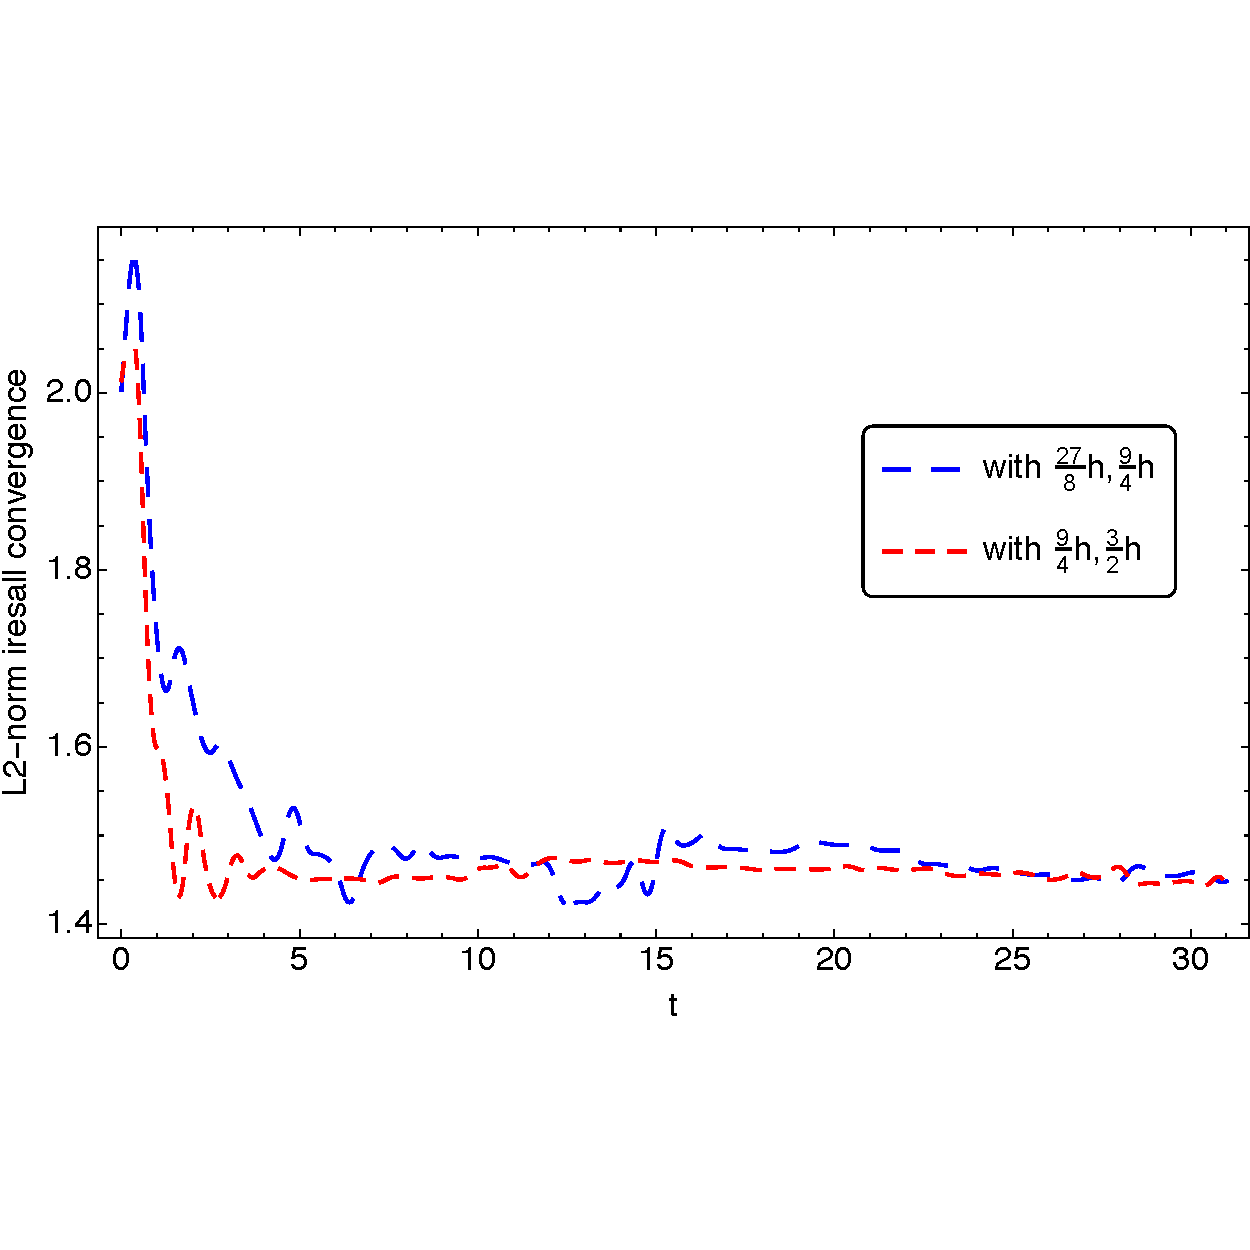
\includegraphics[width=5.0in,clip=true]{plots/timeseries/L2norm_iresallconvergence/fullplottL2normdim2boundedrescaledconvergenceiresallallres.pdf}
\parbox{5.0in}{\caption{Time evolution for $L^2$-norm of convergence factor for independent residual of Einstein equations at different resolutions.
        }\label{fig:L2norm_iresallconvergence-crop}}
\end{figure}

Figure~\ref{fig:L2norm_iresallconvergence-crop} displays the $L^2$-norm of the convergence factor \eqref{eq:qires} for two pairs of resolutions. It clearly shows second order convergence to a solution of the Einstein equations, after an initial transition phase. However, the $L^2$-norm hides the fact that the order of convergence is lower (between 1 and 2) near the AdS boundary due to the fact that we use first order differencing stencils and first order interpolation, through which we impose the Dirichlet boundary conditions (see~\ref{subsec:cartevvarboucon}). More precisely, near-boundary convergence is higher for the lowest pair of resolutions than for the highest one, which shows values closer to 1 (as expected for first order interpolation). This is the reason why the $L^2$-norm of the lowest pair is largest.












\section{Boundary Extrapolation}\label{sec:extrapconvbdy}

As explained in Section~\ref{sec:bouset2}, since the AdS boundary generally does not lie on points of the Cartesian grid, we can only obtain the approximated value of any boundary quantity $f$ through extrapolation from the numerical values of $f$ on grid points near the boundary. In this section we describe how extrapolation is implemented in our scheme with the help of Figure~\ref{fig:lego_circle}. For simplicity, we consider first order extrapolation, i.e., extrapolation from two grid points. The following can be generalized to higher extrapolation orders in a straightforward way. In particular, third order extrapolation is used for the plots in Section~\ref{sec:resbouset}, since this improves the accuracy of the extrapolated numerical values.\footnote{This fact was tested by comparing values obtained with increasing extrapolation order and analytic values, in cases where the latter are known, e.g. boundary scalar field values at $t=0$.}

\begin{figure}[h!]
        \centering
        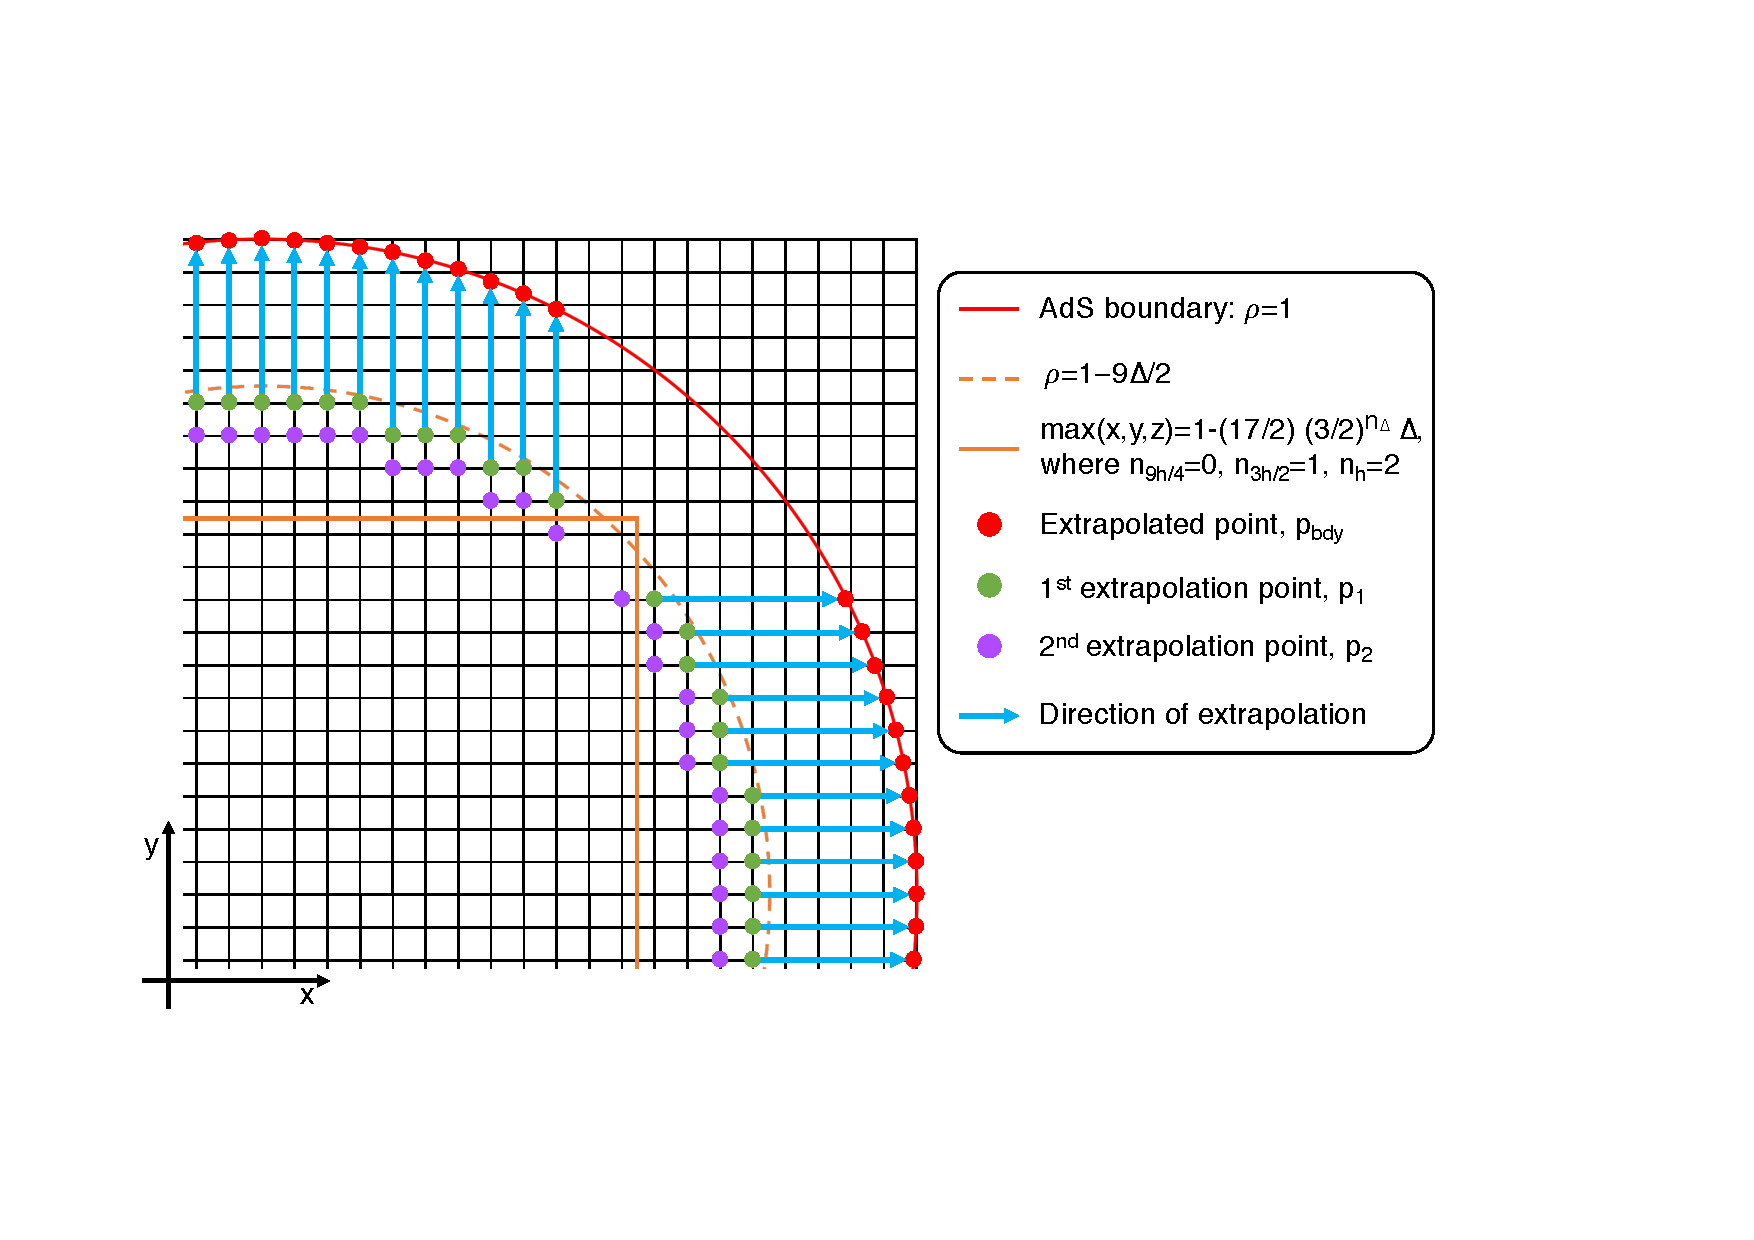
\includegraphics[width=6.1in,clip=true]{plots/lego_circle/Lego_circle_new_noconvergence.pdf}
\parbox{5.0in}{\caption{Visual description of first order extrapolation technique in the first quadrant of a $z=const.$ surface for a grid with spatial refinement $\Delta$.
        }\label{fig:lego_circle}}
\end{figure}

Given a Cartesian grid with spacing $\Delta$, let $f_\Delta$ denote the values of $f$ at bulk grid points and $f^{bdy}_{\Delta}$ denote the extrapolated values of $f$ at boundary points. 
We extrapolate the values $f^{bdy}_{\Delta}$ through the following procedure:
 \begin{enumerate}
 \item Restrict to the points with Cartesian coordinates $(x,y,z)$ satisfying $\rho(x,y,z)<1-9\Delta/2$ (inside the orange dashed line of Figure~\ref{fig:lego_circle}) and $\max(x,y,z)>1-\frac{17}{2}\left(\frac{3}{2}\right)^{n_\Delta}\Delta$ (outside the continuous orange line of Figure~\ref{fig:lego_circle}), where $n_\Delta$ denotes the degree of the three resolutions used for convergence, $n_{9h/4}=0,n_{3h/2}=1,n_{h}=2$ (notice that $\left(\frac{3}{2}\right)^{n_\Delta}\Delta$ is a constant for all three resolutions). We have empirically found that considering points outside of this region in the next steps leads to unphysical or non-converging values.
 \item For any point in the range defined at step 1, identify the coordinate with the largest absolute value, e.g. $x$, and its sign, say $x>0$. If two coordinates have the same absolute value, then we pick $x$ over $y$ and $z$, and $y$ over $z$. Each direction identified in this way is represented by a light blue arrow. Among all the points along the identified direction ($x$ in our example) and within the range of step 1, pick the closest point to the boundary. We denote this point by $p_1$ and its coordinates by $(x_1,y_1,z_1)$. For each direction identified as above, the corresponding $p_1$ point is represented as a green dot in Figure~\ref{fig:lego_circle}.
 \item Consider the nearest point to $p_1$ along the identified axis in the direction of the bulk (decreasing $x$ in the example). We denote this point by $p_2$ and its coordinates by $(x_2,y_2,z_2)$. For each $p_1$ point, the corresponding $p_2$ is represented as a purple dot in Figure~\ref{fig:lego_circle}. In our example $x_2=x_1-\Delta,y_2=y_1,z_2=z_1$.
 \item Use first order extrapolation on $f_\Delta(p_1),f_\Delta(p_{2})$ to determine the value of $f^{bdy}_{\Delta}(p_{bdy})$ where $p_{bdy}$ is the boundary point along the identified axis in the direction of the boundary.  
For each pair $p_1,p_2$, the corresponding $p_{bdy}$ is represented by a red dot in Figure~\ref{fig:lego_circle} and the AdS boundary is represented by a red line.
In our example, $p_{bdy}$ is the point with coordinates $(x_{bdy},y_{bdy},z_{bdy})=(\sqrt{1-y_1^2-z_1^2},y_1,z_1)$ and
 \begin{equation}
 \label{eq:firstordextrap}
 f^{bdy}_{\Delta}(p_{bdy})=\frac{x_{bdy}-x_2}{x_1-x_2}f_\Delta(p_1)+\frac{x_{bdy}-x_1}{x_2-x_1}f_\Delta(p_2).
 \end{equation}
 \end{enumerate}
Figure~\ref{fig:lego_circle} shows that the extrapolated values are not uniformly distributed on the boundary. This issue of our extrapolation scheme is dealt with by linearly interpolating boundary data. We aim to correct this in the future by extrapolating the values at points on a uniform $(\theta,\phi)$ grid with given resolution on the $S^2$ at the boundary.

Notice that, as \eqref{eq:firstordextrap} shows, second order convergence of boundary values $f^{bdy}_{\Delta}$ is a direct consequence of second order bulk convergence of $f_\Delta$, which is confirmed by Figure~\ref{fig:L2norm_iresallconvergence-crop} in our simulations. Despite this fact, some modifications must be made to our extrapolation scheme if we wish to perform explicit convergence tests on our boundary data. We now explain the reason for this and the necessary modifications. We assume the validity of the Richardson expansion [CITE Richardson, L. F. The approximate arithmetic solution by finite differences of physical problems involving differential equations, with applications to the stresses in a masonry dam. Phil. Trans. Roy. Soc., 210:307-357, 1910.] for $f_{\Delta}$ at any grid point $p$,
\begin{equation}
\label{eq:Richexp}
f_\Delta(p)=f(p)+e(p)\Delta^2+\mathcal{O}(\Delta^3),
\end{equation}
where $f(p)$ is the true value of $f$ at $p$ and the rest of the right hand side is the solution error of $f_\Delta(p)$. The validity of this expansion is confirmed by bulk convergence of $f_\Delta$ to $f$.
Then, from \eqref{eq:firstordextrap}, we obtain the Richardson expansion for $f^{bdy}_{\Delta}$ at any extrapolated boundary point $p_{bdy}$:
 \begin{equation}
 \label{eq:bdyRichexp}
 f^{bdy}_{\Delta}(p_{bdy})=f(p_{bdy})+e_{extr}(p_{bdy},p_1,p_2)+e_\Delta(p_1,p_2)\Delta^2+\mathcal{O}(\Delta^3),
 \end{equation}
where the $f(p_{bdy})$ is the true value of $f$ at $p_{bdy}$, $e_{extr}(p_{bdy},p_1,p_2)$ is the error due to the extrapolation approximation and the remaining error terms come from the solution error in $f_\Delta$. The typical  convergence test involves the computation of the convergence factor
\begin{equation}\label{eq:qconv}
Q(p_{bdy})=\frac{1}{\ln(3/2)}\ln\left( \frac{f_{9h/4}(p_{bdy})-f_{3h/2}(p_{bdy})}{f_{3h/2}(p_{bdy})-f_{h}(p_{bdy})} \right)
\end{equation}
at each $p_{bdy}$. We clearly see that $Q(p_{bdy})$ can be expected to asymptote to 2 as $\Delta\rightarrow0$, thus confirming second order convergence in the continuum limit, only if the points $p_1,p_2$ are the same for all 3 resolutions involved. Therefore, our extrapolation scheme must be modified to select pair of bulk points, $p_1$ and $p_2$, for extrapolation that are present in all three grids involved in the convergence test. 
In practice, we saw that boundary convergence follows the trend of bulk convergence only if, in addition to this modification, we restrict to $p_1$ points in the range mentioned in step 1 above. The reason for this should be investigated further. 

Finally, \eqref{eq:bdyRichexp} shows that this type of test does not prove convergence to the true value $f(p_{bdy})$, but rather to its approximation $f(p_{bdy})+e_{extr}(p_{bdy},p_1,p_2)$. For this reason, the convergence test \eqref{eq:qires} cannot be performed at the boundary for functions with vanishing true value (such as $\langle trT \rangle_{CFT}$), because their extrapolated value is not just the term linear in $\Delta^2$ but it also includes the extrapolation error $c_{extr}$. A more detailed analysis must be made to examine the explicit form $e_{extr}(p_{bdy},p_1,p_2)$ and be able to find the rate of convergence to $f(p_{bdy})$. In our study, we simply make the natural assumption that $e_{extr}(p_{bdy},p_1,p_2)$ decreases as we increase resolution, so  $f^{bdy}_{\Delta}(p_{bdy})$ is a sufficiently accurate approximation of $f(p_{bdy})$ for sufficiently high resolution (i.e., sufficiently small $\Delta$).















\section{Poincar\'e Patch}\label{sec:poincare}

%Here we analyze the case of Poincar\'e AdS and display a choice of generalized harmonic source functions that stabilizes evolution in that context. 
Here we follow the prescription of Section~\ref{sec:pre_sta} in the case of Poincar\'e AdS and display a choice of generalized harmonic source functions that stabilizes evolution in that context.
The metric of a Poincar\'e patch of AdS$_4$ can be written in Poincar\'e coordinates $(t,z,x_1,x_2)$ as
\begin{equation}
\label{eq:AdSpoincare}
\hat{g} = \frac{L^2}{z^2} \left( -dt^2 + dz^2 + dx_1{}^2 + dx_2{}^2  \right).
\end{equation}
To include the Poincar\'e horizon $z\rightarrow \infty$ in our computational domain, we compactify the bulk coordinate $z=(1-\rho^2)/\rho^2$ to have the Poincar\'e horizon at $\rho=0$ and the boundary at $\rho=1$, giving the following form for the metric of AdS$_4$
\begin{equation}
\hat{g} = \frac{L^2 \rho^4}{(1-\rho^2)^2} \left( -dt^2 + (4/\rho^6)d\rho^2 + dx_1^2 + dx_2^2  \right).
\end{equation}

Let us now consider asymptotically AdS spacetimes.
Since \eqref{eq:AdSpoincare} is in the form given by the leading order of the FG expansion, \eqref{eqn:FGmetric}, \eqref{eqn:FGbdymetric}, we see that $(t,z,x_1,x_2)$ are FG coordinates.
We can thus read off the fall-offs of the metric components from the rest of the FG expansion. 
Let us now translate these into coordinates $(t,\rho,x_1,x_2)$. The evolved fields consist of the full metric $g_{\mu\nu}$, possibly scalar field matter $\varphi$, and generalized harmonic source functions $H_\mu$.
The fall-offs of the metric components $g_{\mu\nu}$ read the same as \eqref{eq:carbouncondh}, with $f_{\mu\nu}$ functions of $(t,x_1,x_2)$.
Therefore, for coupling with Klein-Gordon matter, the scalar field fall-off preserving the metric asymptotics is given by \eqref{eq:carbouncondphi}, with $c$ function of $(t,x_1,x_2)$. The metric fall-offs also imply the fall-offs of the source function, which are given by \eqref{eq:carbouncondsoufun}, with $f_{\mu}$ functions of $(t,x_1,x_2)$.
As a result of this, the corresponding evolution variables in this Poincar\'e setting are given exactly by the same expressions as we had written in \eqref{eq:gbarcart}, \eqref{eq:phibarcart}, \eqref{eq:soufunb}.

%The evolved fields consist of the full metric $g_{\mu\nu}$, possibly scalar field matter $\varphi$, and generalized harmonic source functions $H_\mu$. 
%The corresponding evolution variables in this Poincar\'e setting give exactly the same expressions as we had written in \eqref{eq:gbarcart}, \eqref{eq:phibarcart}, \eqref{eq:soufunb}.

Using the same steps as in Section~\ref{sec:gauge_choice}, we obtain the following gauge:
\begin{eqnarray}
\label{eq:hbold_poincare}
\bar{H}_{(1)t}&=&\frac{3}{2} \bar{g}_{(1)\text{$t$$\rho $}} \nonumber\\
\bar{H}_{(1)\rho}&=&\frac{3}{2} \bar{g}_{(1) \rho \rho }\nonumber\\
\bar{H}_{(1)x_1}&=&\frac{3}{2} \bar{g}_{(1) \rho x_1 }\nonumber\\
\bar{H}_{(1)x_2}&=&\frac{3}{2} \bar{g}_{(1) \rho x_2 }.
\end{eqnarray}
We have verified that this gauge leads to stable evolution on Poincar\'e AdS$_4$, the results of which will appear in the sequel.



% Bibliography
%-------------------------------------------------------
%\section*{References}
\bibliographystyle{JHEP}
\bibliography{3p1}


\end{document}
